% !TeX program = xelatex
% Main text is mechanically preserved from the formal Google Docs report.
% Compile from this directory: XeLaTeX, BibTeX, XeLaTeX, XeLaTeX.
% Keep references.bib and figures/ beside this file.
\documentclass[11pt,a4paper]{article}
\usepackage[margin=25mm]{geometry}
\usepackage{iftex}
\ifPDFTeX
  \usepackage[T1]{fontenc}
  \usepackage[utf8]{inputenc}
  \usepackage{lmodern}
\else
  \usepackage{fontspec}
  \setmainfont{lmroman10-regular.otf}[BoldFont=lmroman10-bold.otf,ItalicFont=lmroman10-italic.otf,BoldItalicFont=lmroman10-bolditalic.otf]
  \setsansfont{lmsans10-regular.otf}[BoldFont=lmsans10-bold.otf,ItalicFont=lmsans10-oblique.otf]
  \setmonofont{lmmono10-regular.otf}[Scale=MatchLowercase]
\fi
\usepackage{amsmath,amssymb}
\usepackage{graphicx,booktabs,longtable,array,calc}
\usepackage{caption,placeins,needspace}
\usepackage{pdflscape}
\usepackage{etoolbox,titlesec,microtype,ragged2e,textcomp}
\usepackage{xcolor,xurl}
\usepackage[numbers,sort&compress]{natbib}
\usepackage[unicode,hidelinks]{hyperref}
\usepackage{bookmark}
\setcounter{secnumdepth}{0}
\setcounter{tocdepth}{3}
\titleformat{\section}{\large\bfseries}{}{0pt}{}
\titleformat{\subsection}{\normalsize\bfseries}{}{0pt}{}
\titleformat{\subsubsection}{\normalsize\bfseries}{}{0pt}{}
\titlespacing*{\section}{0pt}{2.5ex plus .5ex}{1ex}
\titlespacing*{\subsection}{0pt}{2ex plus .4ex}{.7ex}
\titlespacing*{\subsubsection}{0pt}{1.5ex plus .3ex}{.5ex}
\setlength{\parindent}{0pt}
\setlength{\parskip}{5pt plus 1pt minus 1pt}
\setlength{\emergencystretch}{2em}
\definecolor{captiongray}{RGB}{65,73,80}
\DeclareCaptionFont{reportcaption}{\fontsize{9}{11.5}\selectfont\sffamily\color{captiongray}}
\captionsetup{font=reportcaption,labelfont={bf,color=black},labelsep=period,
  justification=raggedright,singlelinecheck=false,skip=5pt}
\captionsetup[table]{position=top,skip=6pt}
\setlength{\LTcapwidth}{\textwidth}
\setlength{\textfloatsep}{12pt plus 2pt minus 2pt}
\setlength{\floatsep}{10pt plus 2pt minus 2pt}
\setlength{\intextsep}{10pt plus 2pt minus 2pt}
\renewcommand{\topfraction}{0.92}
\renewcommand{\bottomfraction}{0.85}
\renewcommand{\textfraction}{0.07}
\renewcommand{\floatpagefraction}{0.72}
\setcounter{topnumber}{3}
\setcounter{bottomnumber}{2}
\setcounter{totalnumber}{4}
\raggedbottom
\AtBeginDocument{%
  \setlength{\abovedisplayskip}{8pt plus 2pt minus 2pt}%
  \setlength{\belowdisplayskip}{8pt plus 2pt minus 2pt}%
  \setlength{\abovedisplayshortskip}{4pt plus 2pt}%
  \setlength{\belowdisplayshortskip}{6pt plus 2pt minus 2pt}%
}
\setlength{\bibsep}{5pt plus 1pt}
\renewcommand{\bibfont}{\small}
\renewcommand{\bibsection}{\section*{References}\phantomsection
  \addcontentsline{toc}{section}{References}}
\setlength{\tabcolsep}{4pt}
\setlength{\LTpre}{4pt}
\setlength{\LTpost}{8pt}
\widowpenalty=10000
\clubpenalty=10000
\hypersetup{pdftitle={Rainfall Patterns and Short-Term Probabilistic Prediction in Singapore, 2017–2024}}
\begin{document}
\hypersetup{pageanchor=false}
\begin{titlepage}
\centering
\vspace*{25mm}
{\large National University of Singapore\par}
\vspace{15mm}
{\large Course: DSA5208\par}
\vspace{3mm}
{\large Scalable Distributed Computing for Data Science\par}
\vspace{3mm}
{\large Project II\par}
\vspace{20mm}
{\Large\bfseries Rainfall Patterns and Short-Term Probabilistic Prediction in Singapore, 2017–2024\par}
\vspace{20mm}
{\small Group members: Chen Luwei (A0352040X)\quad Dai Peisong (A0351174J)\quad Wan Sihan (A0356906U)\par}
\vfill
{\large Submission date: 18 October, 2026\par}
\vspace*{15mm}
\end{titlepage}
\pagenumbering{roman}
\hypersetup{pageanchor=true,linktoc=all}
\pdfbookmark[0]{Contents}{contents}
\begingroup
\setlength{\parskip}{0pt}
\tableofcontents
\endgroup
\clearpage
\pagenumbering{arabic}


\FloatBarrier

\section*{1. Introduction}
\phantomsection
\addcontentsline{toc}{section}{\numberline{1.}Introduction}


\subsection*{1.1 Background and Objectives}
\phantomsection
\addcontentsline{toc}{subsection}{\numberline{1.1}Background and Objectives}


Rainfall in Singapore exhibits substantial temporal and spatial variability, making it important to understand historical precipitation patterns and assess short-term rainfall risks. This project uses the \textit{Historical Rainfall across Singapore} datasets published by the National Environment Agency (NEA) on \href{https://data.gov.sg/collections/2279/view}{data.gov.sg}~\citep{nea_rainfall}. We analyze eight annual CSV files covering 2017–2024, containing a total of 48,538,713 records before preprocessing. The data consist of five-minute rainfall measurements collected by monitoring stations across Singapore, with rainfall amounts expressed in millimetres (mm).


Each record includes an observation timestamp, station identifier, station name, geographic coordinates, rainfall measurement, and associated update timestamps. All timestamps are provided in Singapore Time (SGT, \(\mathrm{UTC}{+}8\)).


NEA notes that the datasets may contain missing records and have not undergone the quality-control procedures applied to official climate records~\citep{nea_rainfall}. Data auditing and preprocessing are therefore necessary before analysis. The five-minute measurements from stations across Singapore provide a basis for analysing rainfall patterns within and across years and estimating the probability that rainfall over the next 30 minutes will exceed a specified threshold.


This project has two objectives. First, it aims to characterize rainfall patterns within individual years and examine their variation across 2017–2024, focusing on seasonal, temporal, and spatial differences in rainfall distribution. Second, it aims to develop a predictive model that estimates the probability that cumulative rainfall at a monitoring station will exceed a specified threshold over the next 30 minutes.


\subsection*{1.2 Project Overview}
\phantomsection
\addcontentsline{toc}{subsection}{\numberline{1.2}Project Overview}


The project follows a structured workflow consisting of data preparation, exploratory analysis, feature engineering, predictive modeling, and evaluation.


First, the raw rainfall datasets are audited for missing values, duplicate records, invalid measurements, and inconsistencies in station information. The observation timestamps are then standardized to a consistent five-minute grid. Then the validated data is converted into Parquet format for efficient processing using Apache Spark.


Next, exploratory data analysis examines rainfall patterns at different temporal and spatial scales, including seasonal and diurnal variations, interannual differences, station-level differences, spatial correlations, and rainfall persistence. These findings guide feature engineering by identifying relevant calendar patterns, station characteristics, and temporal and spatial relationships in rainfall.


For the prediction task, training labels are created by assigning each observation to one of nine categories based on the total rainfall recorded at the same station over the following 30 minutes. Predictive features capture station characteristics, calendar information, recent rainfall, and rainfall at neighboring stations. Multinomial logistic regression and random forest models are trained to estimate the probability of each rainfall category. These probabilities are then used to estimate the probability that cumulative rainfall over the next 30 minutes will exceed a specified threshold.


Finally, data from 2017–2022, 2023, and 2024 are used for training, validation, and testing, respectively. The models are compared with baseline forecasts in terms of predictive performance and probability calibration.


\FloatBarrier

\section*{2. Data and Computing Environment}
\phantomsection
\addcontentsline{toc}{section}{\numberline{2.}Data and Computing Environment}


\subsection*{2.1 Dataset Description}
\phantomsection
\addcontentsline{toc}{subsection}{\numberline{2.1}Dataset Description}


The dataset used in this project is obtained from the \textit{Historical Rainfall across Singapore} collection published by the National Environment Agency (NEA) on \href{https://data.gov.sg/collections/2279/view}{data.gov.sg}~\citep{nea_rainfall}. Across the eight annual CSV files, the raw data comprise 48,538,713 observations from 91 unique monitoring stations. The number of stations with recorded observations in each year ranges from 54 to 80.


Rainfall measurements represent the total rainfall accumulated over five-minute intervals and are expressed in millimetres (mm). Each record includes station information, geographic coordinates, and an observation timestamp in Singapore Time (SGT, \(\mathrm{UTC}{+}8\)). The observation timestamp provides the temporal reference for rainfall analysis, while update timestamps are examined during data-quality auditing to assess delays between observations and record updates.


The number of observations and reporting stations varies across years. Table 1 summarizes these annual counts, providing an overview of data coverage before preprocessing.


\Needspace{4\baselineskip}
\begingroup
\small
\setlength{\parskip}{0pt}
\renewcommand{\arraystretch}{1.18}
\begin{longtable}{@{}>{\raggedright\arraybackslash}p{(\linewidth-4\tabcolsep)*\real{0.16}}>{\raggedright\arraybackslash}p{(\linewidth-4\tabcolsep)*\real{0.4}}>{\raggedright\arraybackslash}p{(\linewidth-4\tabcolsep)*\real{0.44}}@{}}
\caption*{\textbf{Table 2.1.} Annual overview of the raw rainfall dataset.}\\
\toprule
\textbf{Year} & \textbf{Number of observations} & \textbf{Number of reporting stations} \\
\midrule
\endfirsthead
\toprule
\textbf{Year} & \textbf{Number of observations} & \textbf{Number of reporting stations} \\
\midrule
\endhead
2017 & 5,256,106 & 62 \\
2018 & 4,594,246 & 56 \\
2019 & 5,026,862 & 54 \\
2020 & 6,334,473 & 80 \\
2021 & 7,044,646 & 76 \\
2022 & 7,133,230 & 72 \\
2023 & 6,742,890 & 74 \\
2024 & 6,406,260 & 70 \\
\bottomrule
\end{longtable}
\endgroup


\textit{Note: Counts refer to the raw data before preprocessing. Station counts represent distinct station identifiers within each year.}


NEA notes that the datasets may contain missing records and have not undergone the quality-control procedures applied to official climate records~\citep{nea_rainfall}. Missing observations must therefore be distinguished from recorded zero rainfall: a zero value indicates no measured rainfall during the corresponding interval, whereas a missing observation provides no measurement for that interval. These limitations motivate the data validation and preprocessing described in the following section.


\subsection*{2.2 Computing Environment}
\phantomsection
\addcontentsline{toc}{subsection}{\numberline{2.2}Computing Environment}


Initial data validation and temporal preparation were performed locally on a MacBook Pro running macOS 26.6.2, with a 15-core Apple M5 Pro processor and 48 GB of physical memory. The preprocessing environment used Python 3.14.7, OpenJDK 17.0.20.1, and Apache Spark/PySpark 4.2.0. [Windows TBD…]


The project runs Apache Spark in local mode on a single machine. Parallelism is provided by local worker threads rather than a distributed cluster. The source code specifies the following resource settings.


\Needspace{4\baselineskip}
\begingroup
\small
\setlength{\parskip}{0pt}
\renewcommand{\arraystretch}{1.18}
\begingroup
\small
\setlength{\tabcolsep}{4pt}
\renewcommand{\arraystretch}{1.15}
\setlength{\LTleft}{0pt}
\setlength{\LTright}{0pt}

\begin{longtable}{
    >{\raggedright\arraybackslash}
    p{\dimexpr0.40\linewidth-2\tabcolsep\relax}
    >{\raggedright\arraybackslash}
    p{\dimexpr0.18\linewidth-2\tabcolsep\relax}
    >{\raggedright\arraybackslash}
    p{\dimexpr0.21\linewidth-2\tabcolsep\relax}
    >{\raggedright\arraybackslash}
    p{\dimexpr0.21\linewidth-2\tabcolsep\relax}
}

\toprule
\textbf{Stage}
& \textbf{Execution mode}
& \textbf{Driver memory}
& \textbf{Shuffle partitions} \\
\midrule
\endfirsthead

\toprule
\textbf{Stage}
& \textbf{Execution mode}
& \textbf{Driver memory}
& \textbf{Shuffle partitions} \\
\midrule
\endhead

Data validation and temporal preparation
& \texttt{local[4]}
& Spark default (1 GB)
& Spark default (200) \\

Task 1 aggregation and station-matrix construction
& \texttt{local[4]}
& 4 GB
& 32 \\

Task 2 labels and features (notebooks 01--06, 08), own machine
& \texttt{local[8]}
& 10 GB
& 96 \\

Task 2 tuning, final fit and test (notebooks 07, 09, 10),
cloud VM with 32 vCPU and 252 GB RAM
& \texttt{local[32]}
& $[\ldots]$
& $[\ldots]$ \\

\bottomrule
\end{longtable}

\endgroup
\endgroup


These are source-code settings and may be overridden by command-line arguments or environment variables. The Task 2 models confirm Spark 4.2.0. Task 2 notebook metadata records Python 3.12.2 for notebooks 01–08 and Python 3.11.2 for notebooks 09–10.


Raw observations were stored as annual CSV files. Prepared observations were written as Snappy-compressed Parquet files organised by source year. The station matrix, feature tables, and modelling datasets also used Parquet, while summary results were exported as CSV files. Task 1 used NumPy and pandas for data analysis and Matplotlib for visualisation~\citep{numpy_docs,pandas_docs,matplotlib_docs}. Task 2 used Spark MLlib for modelling. All Spark sessions used the Asia/Singapore time zone. Arrow-based spatial feature calculations limited batches to 1,000 records.


\subsection*{2.3 Use of Apache Spark}
\phantomsection
\addcontentsline{toc}{subsection}{\numberline{2.3}Use of Apache Spark}


Apache Spark provides the main framework for data preparation, large-scale aggregation, and predictive modelling~\citep{spark_sql,spark_ml}. Spark DataFrames are used to read the annual CSV files, convert field types, validate observations, align timestamps, and save the prepared data as Parquet. Aggregations assess missingness, duplicate records, and station coverage, while joins associate observations with metadata and quality-control flags.


\subsubsection*{2.3.1 Task 1 Rainfall Pattern Analysis}
\phantomsection
\addcontentsline{toc}{subsubsection}{\numberline{2.3.1}Task 1 Rainfall Pattern Analysis}


For Task 1, Spark generates summary tables and a station rainfall matrix on a regular five-minute time grid. The matrix preserves missing observations and is stored in Snappy-compressed Parquet format. NumPy uses this matrix to calculate pairwise lagged correlations efficiently through matrix products. The revised temporal and persistence analyses also derive summaries from the matrix. Statistical analysis and visualisation are performed locally using Python libraries.


\subsubsection*{2.3.2 Task 2 Rainfall Prediction}
\phantomsection
\addcontentsline{toc}{subsubsection}{\numberline{2.3.2}Task 2 Rainfall Prediction}


Task 2 estimates the probability that rainfall at a station will exceed a specified threshold over the next 30 minutes. Spark calculates future rainfall targets and recent rainfall features for each station. It then combines these with station, time, and neighbour features. Neighbour features are computed using NumPy through Spark’s mapInPandas.


Spark MLlib pipelines train multinomial logistic regression and random forest classifiers. Spark builds three baseline forecasts: constant, climatology, and persistence. Model performance is evaluated using log loss, AUC-PR, Brier score, and ranked probability score. Reliability summaries compare predicted probabilities with observed event frequencies.


\FloatBarrier

\section*{3. Data Quality Assessment and Preparation}
\phantomsection
\addcontentsline{toc}{section}{\numberline{3.}Data Quality Assessment and Preparation}


\subsection*{3.1 Data Validation}
\phantomsection
\addcontentsline{toc}{subsection}{\numberline{3.1}Data Validation}


We first employed the script \texttt{rainfall\_audit.py} to obtain an overview of the full dataset integrity, checking missing values, duplicate keys, invalid values, etc. The script performs these checks with Apache Spark. In total, we have 48, 538, 713 observations across 91 unique stations, and among them we found that the overall integrity of data is well held, as there are no duplicate keys, no disagreement between date and timestamp, etc., yet there is one major issue of our concern, the coverage. We found the lack of coverage mainly from two dimensions, the intra-year continuity of records, and continuity within the whole observation window from 2017 to 2024. For example, for every individual year, there is at least one station that has intra-year coverage below \(80\%\) of the time. We will further elaborate patterns of coverage in the coming section. Meanwhile, we noticed some changes took place in the station names, yet that creates little effect as we do not intend to encode them as features for training. 


\textbf{Table 2. Data-quality checks, findings, and treatment decisions.}


\subsection*{3.2 Temporal Alignment and Duplicate Resolution}
\phantomsection
\addcontentsline{toc}{subsection}{\numberline{3.2}Temporal Alignment and Duplicate Resolution}


Each observation in the dataset is expected to fall on a five-minute grid (e.g. 01:10:00). However, there are some disagreements regarding this convention worth our treatment. We found that in 2017, there are 1,775,327 threads of observations recorded at second 59, and for 86 of these records, the same reading was also published under the correct convention, namely the identical rainfall events were recorded with different timestamps in the original dataset. We therefore shifted each of these observations at second 59 forward while keeping the original timestamp in a separate column, and for these 86 duplicate pairs, we kept the correct ones. After the alignment, the dataset contains 48, 538, 627 observations in total, each with a unique station-time key.


\subsection*{3.3 Missing Observations and Coverage}
\phantomsection
\addcontentsline{toc}{subsection}{\numberline{3.3}Missing Observations and Coverage}


In our data preprocessing, the indicator coverage is the share of expected five-minute observations that a station reported over a period. For example, the monthly coverage is then defined as 
\[
\mathrm{coverage}=\frac{\text{number of observations}}{\text{days in the month}\times288}.
\]
Figure~\ref{fig:coverage}(a) provides us with a panoramic view of data coverage below, suggesting two ways in which the raw data fall short. First, when we filtered out observations from stations having monthly coverage below \(90\%\), there are 11 out of the 96 months no stations reaching this coverage threshold, and most of them lie in 2018-2020. These gaps mainly come from island-wide interruptions in rainfall tracking instead of individual stations. Second, Figure~\ref{fig:coverage}(a) suggests that fewer stations pass the \(90\%\) check before mid-2020. This reflects that the station network is systematically smaller, with 54 nodes reporting in 2019 and 80 nodes in 2020. This is visible also from the grey area in the bottom left corner of Figure~\ref{fig:coverage}(b). However, the coverage checks are mainly diagnostic, as they are used as a cutoff standard only in statistical analysis of Task 1. In the model training and prediction of Task 2, we applied no coverage filter but relevant data manipulations discussed in the corresponding section below.


\begin{figure}[!htbp]
\centering
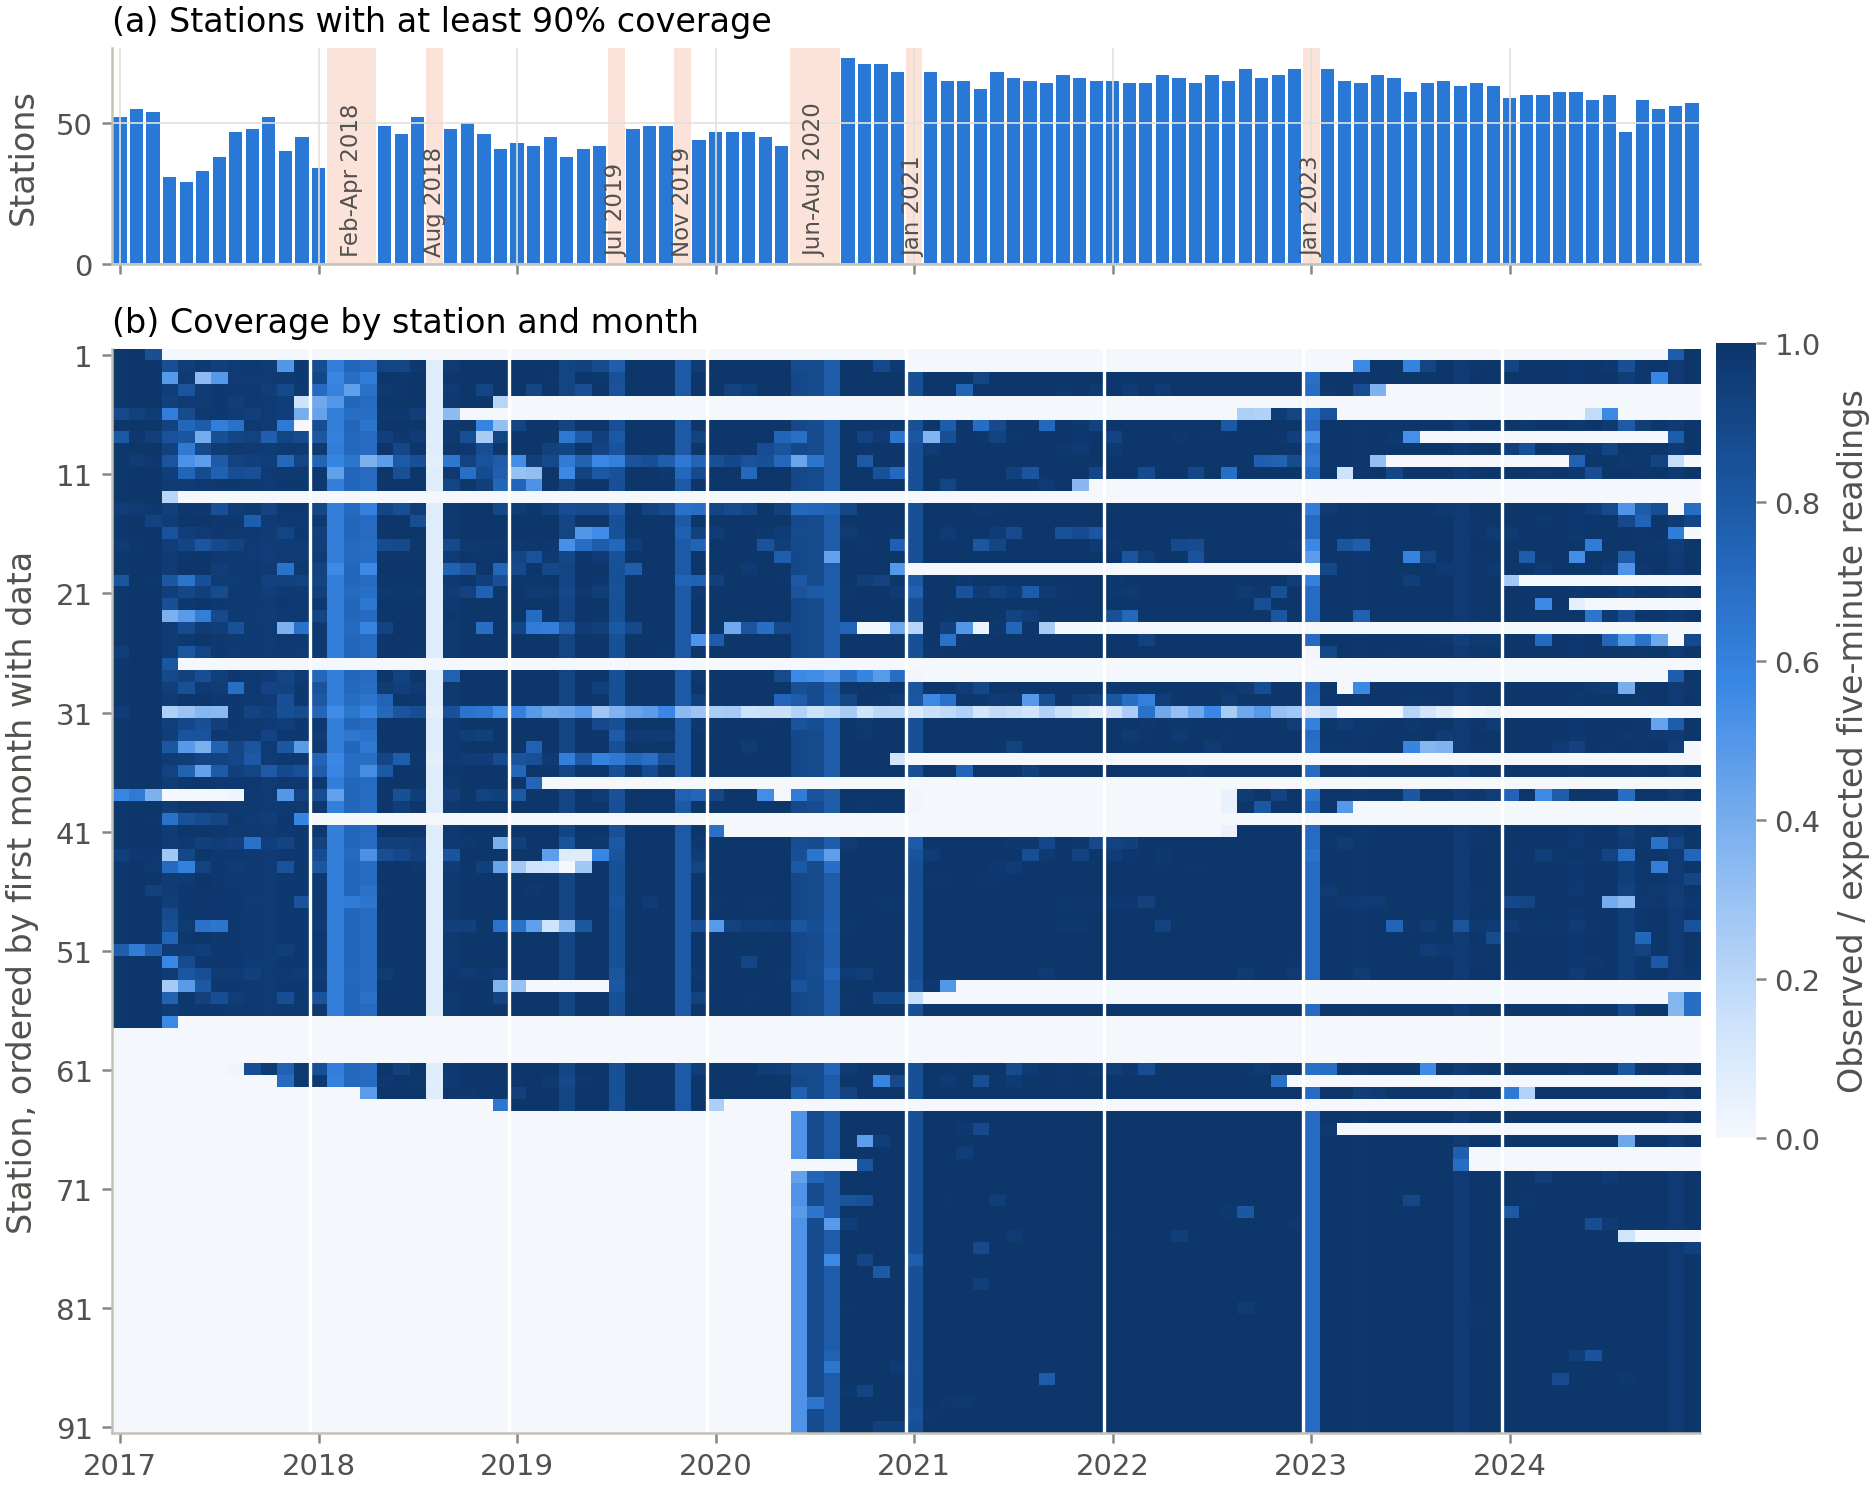
\includegraphics[width=0.94\linewidth,height=0.43\textheight,keepaspectratio]{figures/00_coverage_by_month.png}
\caption{Data coverage of the 91 stations, 2017-2024. (b) Share of the expected five-minute readings each station reported in each month; stations are ordered by their first month with data. (a) Number of stations with at least \(90\%\) coverage in each month. In the 11 shaded months no station reached \(90\%\) (network-wide outages), so these months are missing from every monthly analysis; the gaps reflect recording, not dry weather.}
\label{fig:coverage}
\end{figure}


\subsection*{3.4 Analysis-Specific Data Preparation}
\phantomsection
\addcontentsline{toc}{subsection}{\numberline{3.4}Analysis-Specific Data Preparation}


We will briefly introduce how we conducted our preparation work before giving detailed analysis below. For Task1, we analyzed rainfall patterns across months and years, so it is necessary to keep only station-months with at least \(90\%\) coverage and station-years with at least \(80\%\) for drawing general conclusions, though the exact choice of thresholds bear no statistical significance here. On the contrary, the training and prediction work in Task 2 in general needs a complete future window, so applying no coverage filtering preserves continuity in observations.   


\FloatBarrier

\section*{4. Task 1: Exploration of Rainfall Patterns}
\phantomsection
\addcontentsline{toc}{section}{\numberline{4.}Task 1: Exploration of Rainfall Patterns}


\subsection*{4.1 Analytical Approach}
\phantomsection
\addcontentsline{toc}{subsection}{\numberline{4.1}Analytical Approach}


Here we introduce some important definitions of measurement of our concern and they are critical in understanding our interpretations of rainfall patterns below. First of all, as iteratively suggested, the basic unit of rainfall records is the five-minute reading, and we call it a wet reading if it is above zero, or \(0\,\mathrm{mm}\) and a wet day if its rain is at least \(1\,\mathrm{mm}\). Then, the stations’ reports normally do not fill up the entire five-minute grid throughout a day, as missing values occur in some of the slots, making stations incomparable between each other. To address this issue, we define a normalized rainfall rate, 
\[
\mathrm{rate}(s,p)=\frac{\text{sum of rain observed in }p\times288}{\text{number of observed readings in }p}
\]
for any station \(s\), to denote the mean rain per observed interval in daily scale. 


\subsection*{4.2 Seasonal Patterns Within a Year}
\phantomsection
\addcontentsline{toc}{subsection}{\numberline{4.2}Seasonal Patterns Within a Year}


We first explore how rainfall patterns change across months of a year, and ask one core question that if the seasonal cycle we identify is consistent across years. For each month, we take the normalized rainfall rate defined above for each station, keep only the stations whose monthly coverage is at least \(90\%\), and average them. According to Figure~\ref{fig:seasonal-cycle}(a), we found that the monthly rates of individual years fluctuate widely, yet the average across years (the blue curve) suggests some seasonal structure, dips occurring in February and in the summer, while peaks are clearest in November and April. Statistically, only November stands out, as it lies \(3.4\,\mathrm{mm}\) per day above the average month, whereas no other month remains significant after correcting for twelve comparisons. This is because we test twelve months at once, and some of them would look significant by chance, so we adjust the \(p\)-values with the Holm method (using the \texttt{multipletests} function of statsmodels)~\citep{statsmodels_holm}. Overall, we may thus conclude that the cycle is more systematic than the year-to-year difference.

\begin{figure}[!htbp]
\centering
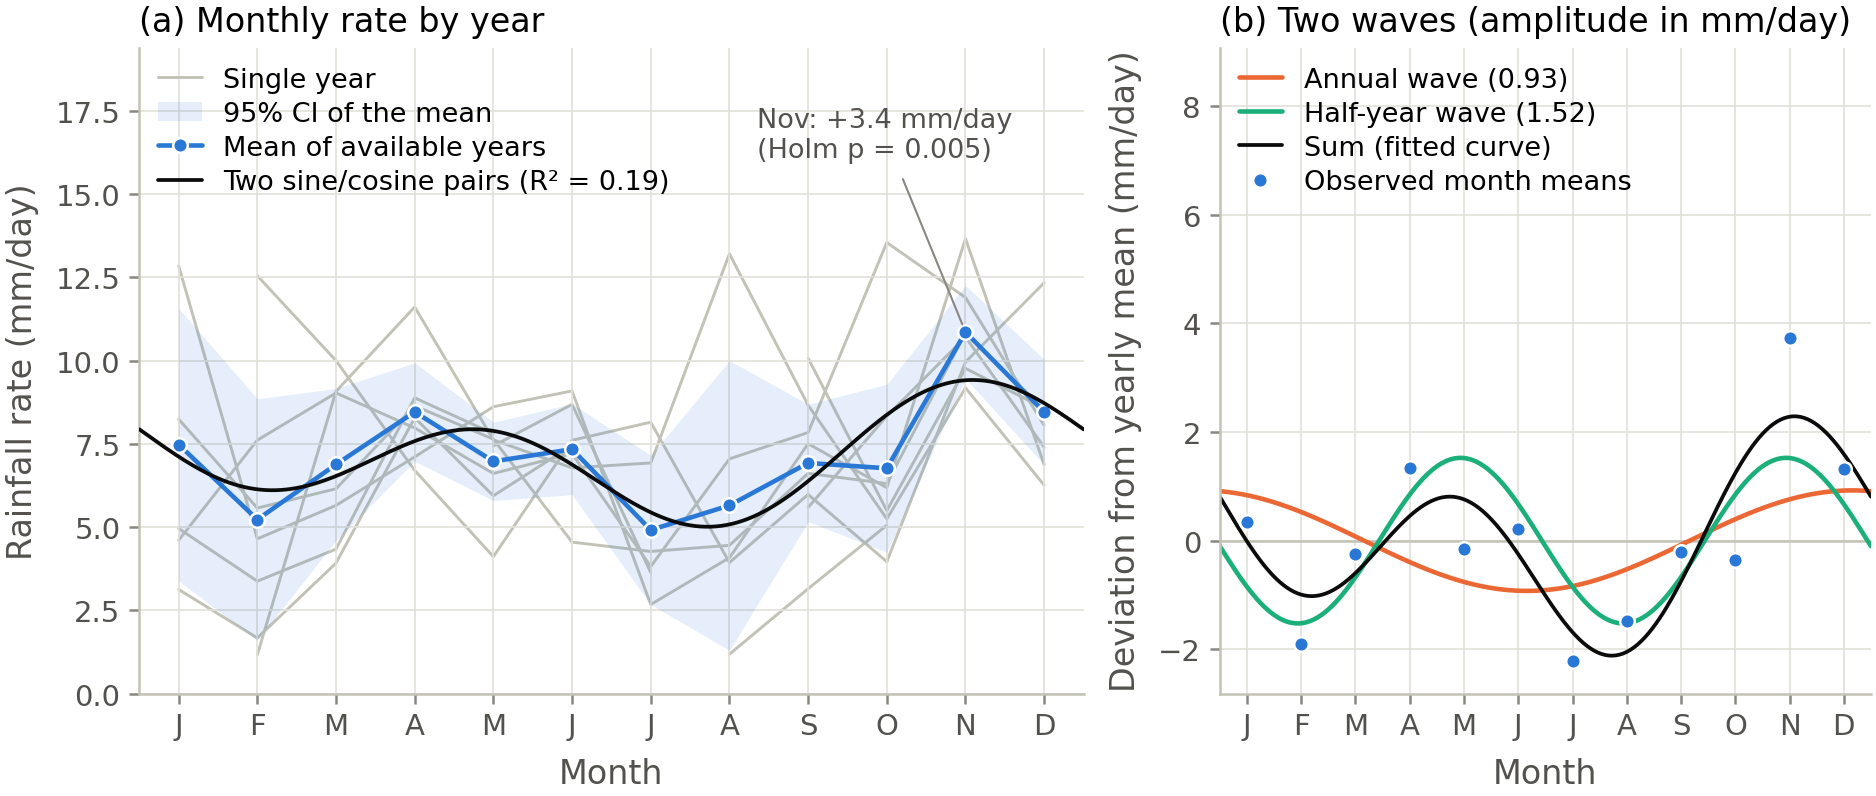
\includegraphics[width=0.96\linewidth,height=0.37\textheight,keepaspectratio]{figures/10_seasonal_cycle.png}
\caption{Seasonal cycle of the network-mean rainfall rate. (a) Rate in each month of each year (grey), the mean of the available years with its \(95\%\) confidence interval (blue), and a regression on two sine/cosine pairs (black). (b) The fitted curve is the sum of an annual and a half-year wave; dots are the observed month's mean relative to the yearly mean. In a two-way ANOVA, month of year explains \(28\%\) of the monthly variation (\(p=0.006\)), year \(10\%\) (\(p=0.18\)), and \(62\%\) is left to weather specific to one month of one year; a permutation test that shuffles months within years confirms the seasonality (\(p=0.006\)).}
\label{fig:seasonal-cycle}
\end{figure}


We then regressed the observed monthly means of rainfall rate on sine and cosine terms of the month. Particularly, we encoded the month with sine and cosine, as we believe that it helps keep December next to January temporally, which an integer month indicator would not. Shown in Figure~\ref{fig:seasonal-cycle}(b), switching from one annual wave to an additional half-year wave grants us an increase in \(R^2\) from 0.05 to 0.19. This convinced us that it is promising to describe the cycle with a few parameters (four coefficients in total). We therefore conclude that there is a real seasonal cycle, though modest statistically, and that it is useful to encode time with sine and cosine in the prediction model. Whether it helps the 30-minute prediction is still unknown to us, because these results describe monthly averages rather than short windows. 


\subsection*{4.3 Interannual Differences, 2017–2024}
\phantomsection
\addcontentsline{toc}{subsection}{\numberline{4.3}Interannual Differences, 2017–2024}


Next, we ask whether rainfall shows any interannual structure and what we can learn from it. We again take the normalized rainfall rate of each month, averaged over the stations with at least \(90\%\) coverage, and check whether it lies above or below the average of the same calendar month across the eight years unanimously. As Figure~\ref{fig:annual-anomalies}(a) shows, in every year except 2019, we have a roughly even share of wetter and drier months, with 4 to 6 wetter months among 8 to 12 months with enough coverage. However, if we further investigate the year of 2019, 8 of the 10 valid months are drier than usual. Its annual mean is \(4.8\,\mathrm{mm}\) a day, against 6.8 to \(8.0\,\mathrm{mm}\) a day in other years (Figure~\ref{fig:annual-anomalies}(b)). Here, it is worth noting that the annual means in Figure~\ref{fig:annual-anomalies}(b) requires a yearly coverage above \(80\%\). This is a lower cutoff than the monthly one because in 2018 no station reaches \(90\%\) over the whole year. Indeed, this larger tolerance for missing values in a particular year will not reject the dip in 2019, as it persists when a higher cutoff is applied.


\begin{figure}[!htbp]
\centering
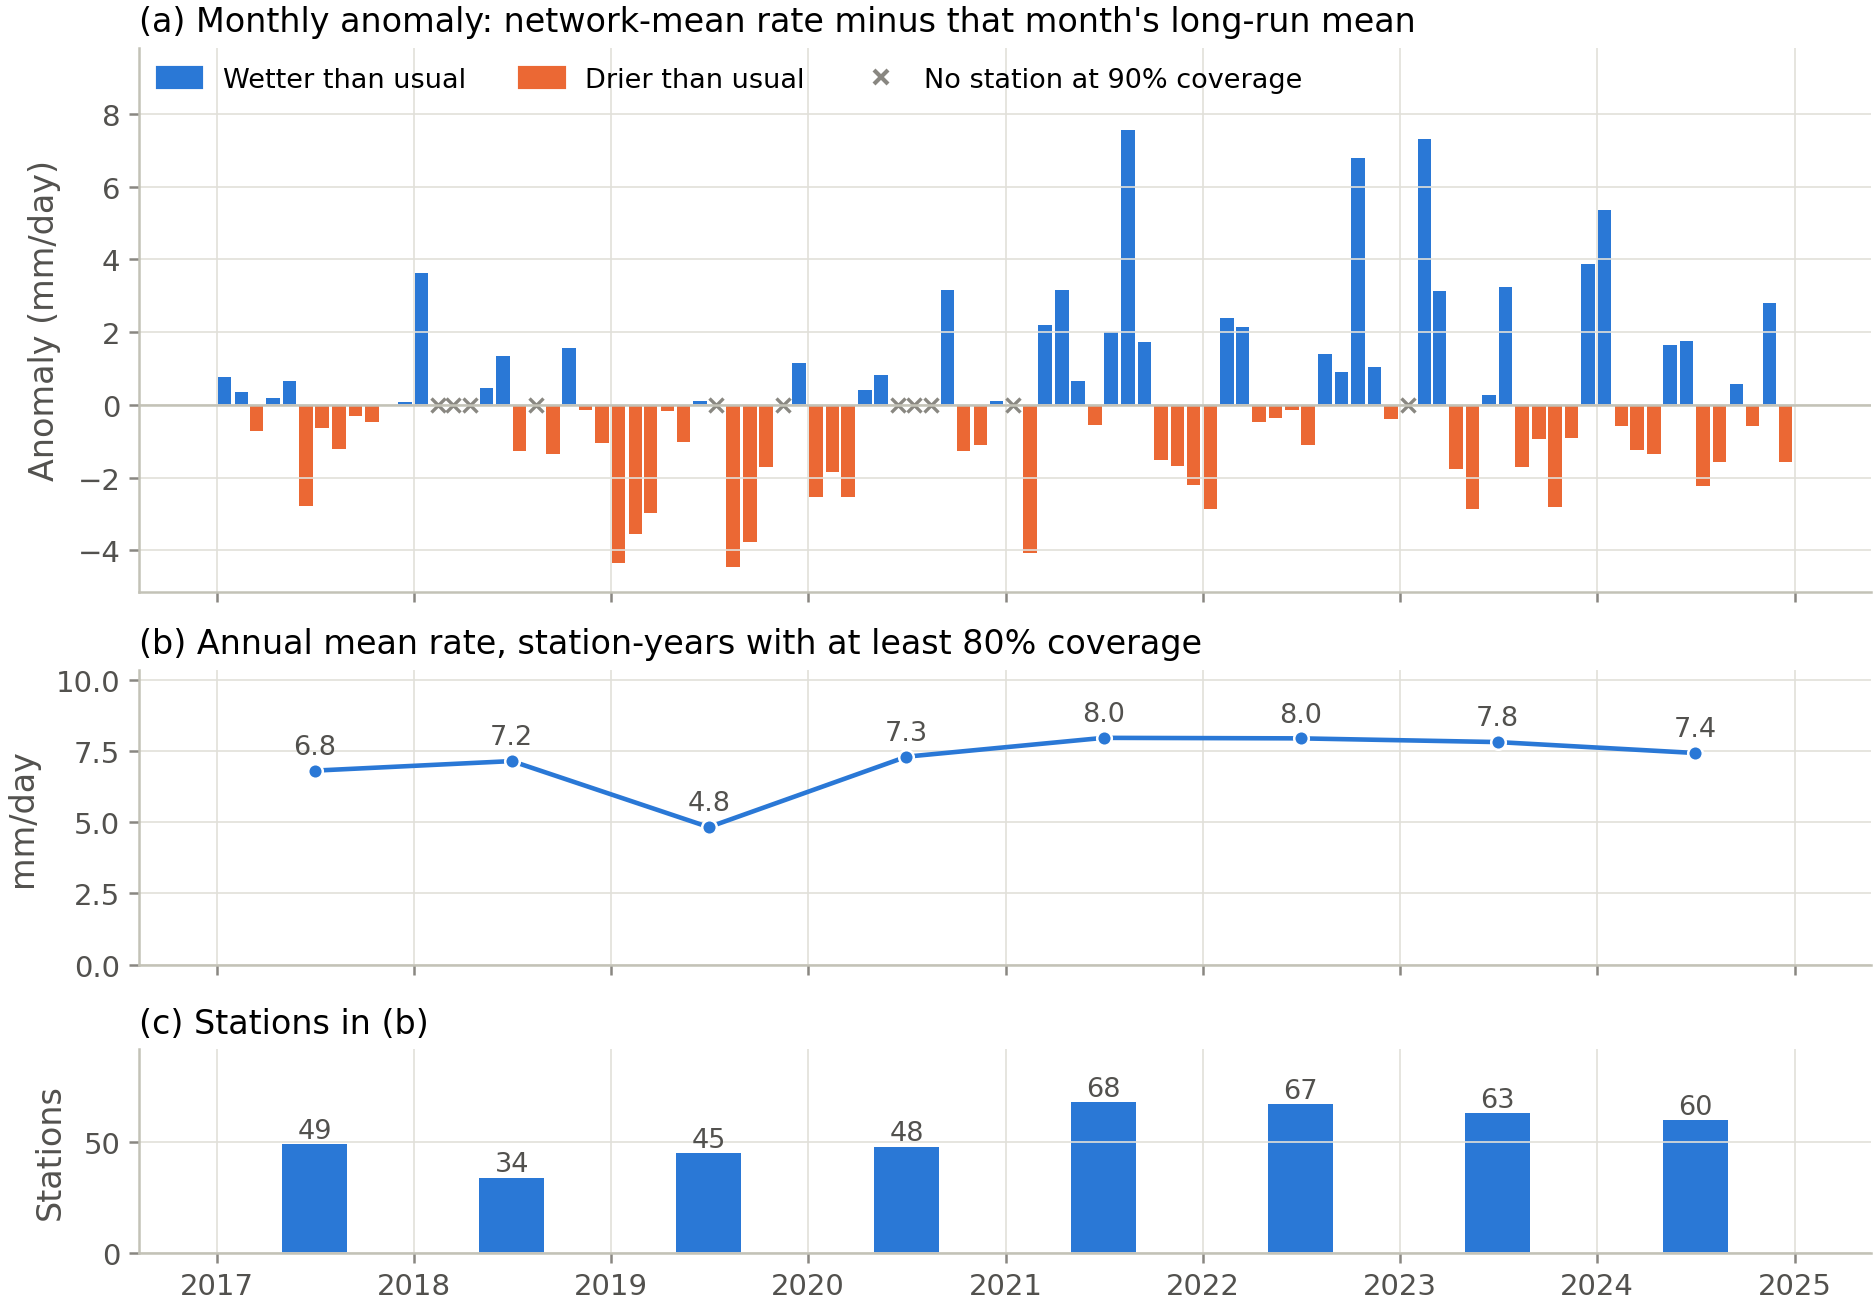
\includegraphics[width=0.92\linewidth,height=0.44\textheight,keepaspectratio]{figures/11_anomalies.png}
\caption{Interannual rainfall anomalies and annual mean rainfall rates, 2017–2024.}
\label{fig:annual-anomalies}
\end{figure}


Another pattern standing out is that across years, large deviations of a month from its yearly average are rare. Apart from the drier 2019, they appear as spikes and troughs. These signs thus lead us to believe that it is not worth building features for identifying a specific year in our later implementation, as little interannual difference is shown. However, it is also true that with only eight years of data, we cannot further comment on any long-term trend.


\subsection*{4.4 Diurnal Patterns}
\phantomsection
\addcontentsline{toc}{subsection}{\numberline{4.4}Diurnal Patterns}


Having examined the yearly and monthly patterns, we now turn to the daily cycle. It is commonly believed that the afternoon is the wetter part of the day~\citep{mss_climate}. To describe how wet a period is, we may decompose it into two factors, how hard it rains when it does (intensity) and how often it rains (frequency). We summed up the normalized rainfall rate within each hour and averaged over years. As Figure~\ref{fig:diurnal}(a) shows, the daily pattern is clearer and more consistent than the monthly one, as the same sine/cosine pairs that explain \(19\%\) of the monthly variation now explain \(73\%\) of the hourly variation, and three pairs reach \(R^2=0.82\). In particular, we found that rainfall occurring between 1pm to 7pm in the afternoon creates a peak, roughly \(48\%\) of the daily total. 


In order to further investigate this specific period, we first pooled the amount of rainfall rate of each hour in a day over years and divided them by the 24-hour mean, resulting in a relative strength of diurnal rainfall. As suggested above, we split the pooled rate into frequency, the share of wet five-minute readings in an hour, and intensity, the rain per wet reading. Thus, according to Figure~\ref{fig:diurnal}(b), the rate (grey) peaks at about 2.6 times as heavy. The perception of a wetter afternoon is therefore driven mainly by more frequent rain, and only to a smaller extent by heavier rain. 


However,a pattern averaged over the whole year might hide differences between seasons. As the peak hours are stable across years, we then examine whether such patterns also hold across months. 


\begin{figure}[!htbp]
\centering
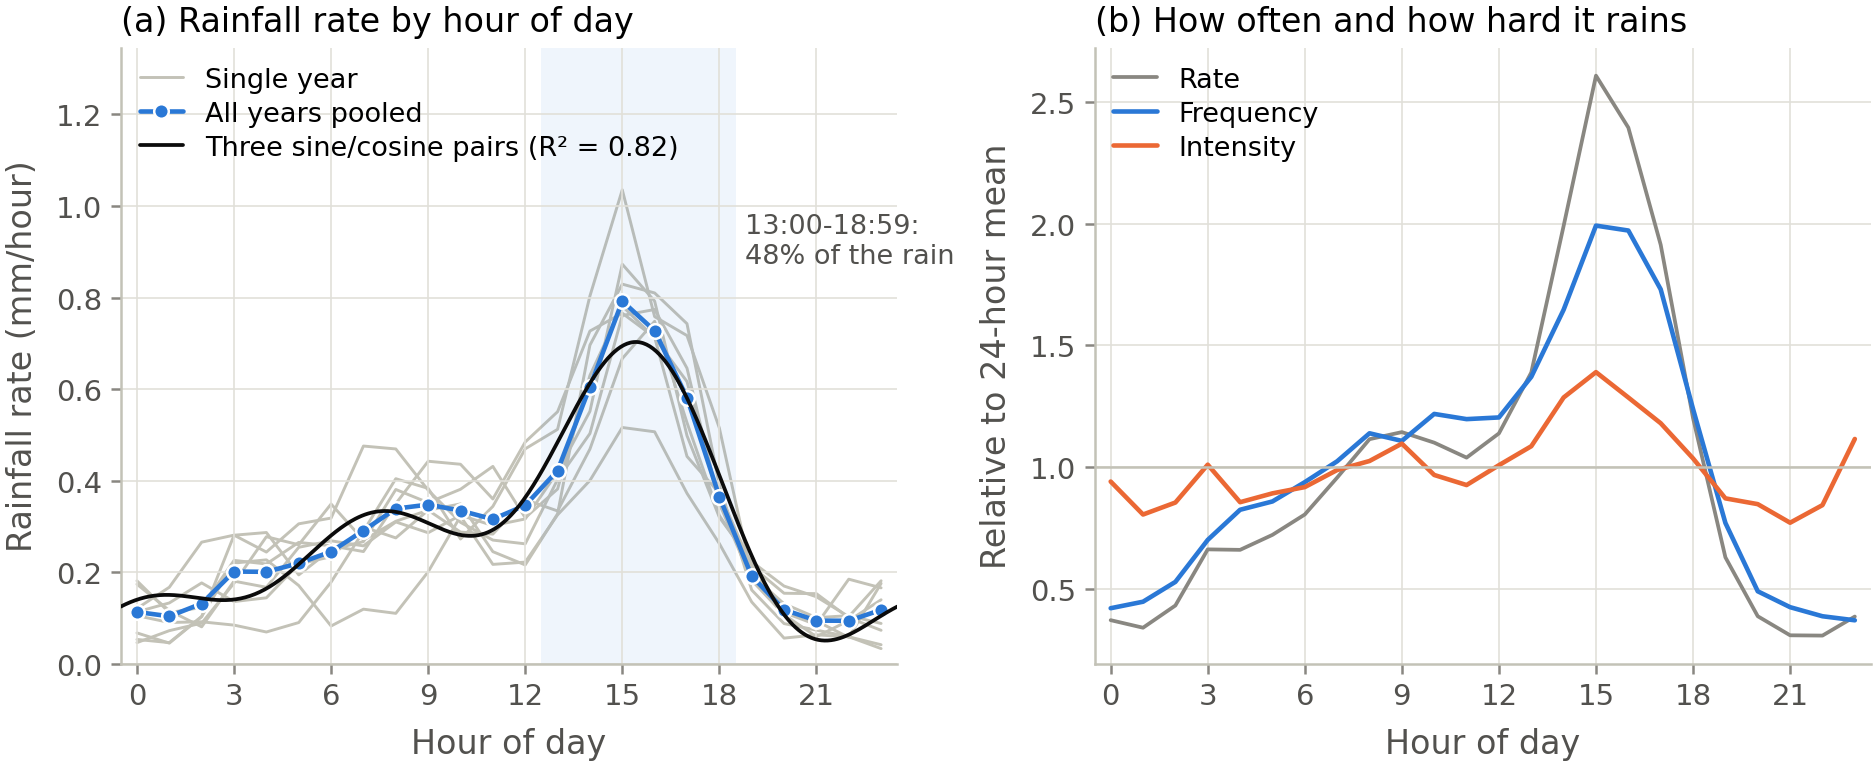
\includegraphics[width=0.96\linewidth,height=0.36\textheight,keepaspectratio]{figures/12_diurnal.png}
\caption{Daily cycle of rainfall, Singapore time. (a) Mean rate per hour in each year (grey), pooled over all years (blue), and a regression on three sine/cosine pairs (black; \(R^2=0.82\) against 0.86 for 24 hour dummies) that peaks at about 15:24. \(48\%\) of the daily rain falls between 13:00 and 18:59, and the peak hour is 15:00 or 16:00 in every year. (b) The rate split into how often it rains (share of wet five-minute readings) and how hard (rain per wet reading), each relative to its 24-hour mean: at 15:00 rain is 5.1 times as frequent as at 22:00 but only 1.6 times as heavy.}
\label{fig:diurnal}
\end{figure}


Slicing the rainfall rate by months instead provides us with a different picture (Figure~\ref{fig:month-hour}(a)) . The claim of a wetter afternoon is now challenged by months from May to October, as there is no distinct afternoon peak and the rain is spread over the morning instead. We may quantify this shift in dynamics through Figure~\ref{fig:month-hour}(b), where we calculated the share of each month’s rain that falls in the afternoon (13:00-18:59) and in the morning (04:00-09:59). The two shares mirror each other. What is presented here is indeed consistent with Sumatra squalls, as lines of thunderstorms that reach Singapore in the pre-dawn and morning hours mainly during the southwest monsoon~\citep{mss_climate}, causing the morning share to rise significantly from June to September. 


Therefore, on a relatively microscopic view, we draw on two core findings about the daily rainfall pattern. First, the hour of the day mostly decides whether it rains rather than how much, and this is helpful in learning rainfall patterns within lower thresholds. Second, the shape of the daily cycle depends on the season, or month, so it is necessary to encode the hour, seasonality explicitly or implicitly according to models’ nature.  


\begin{figure}[!htbp]
\centering
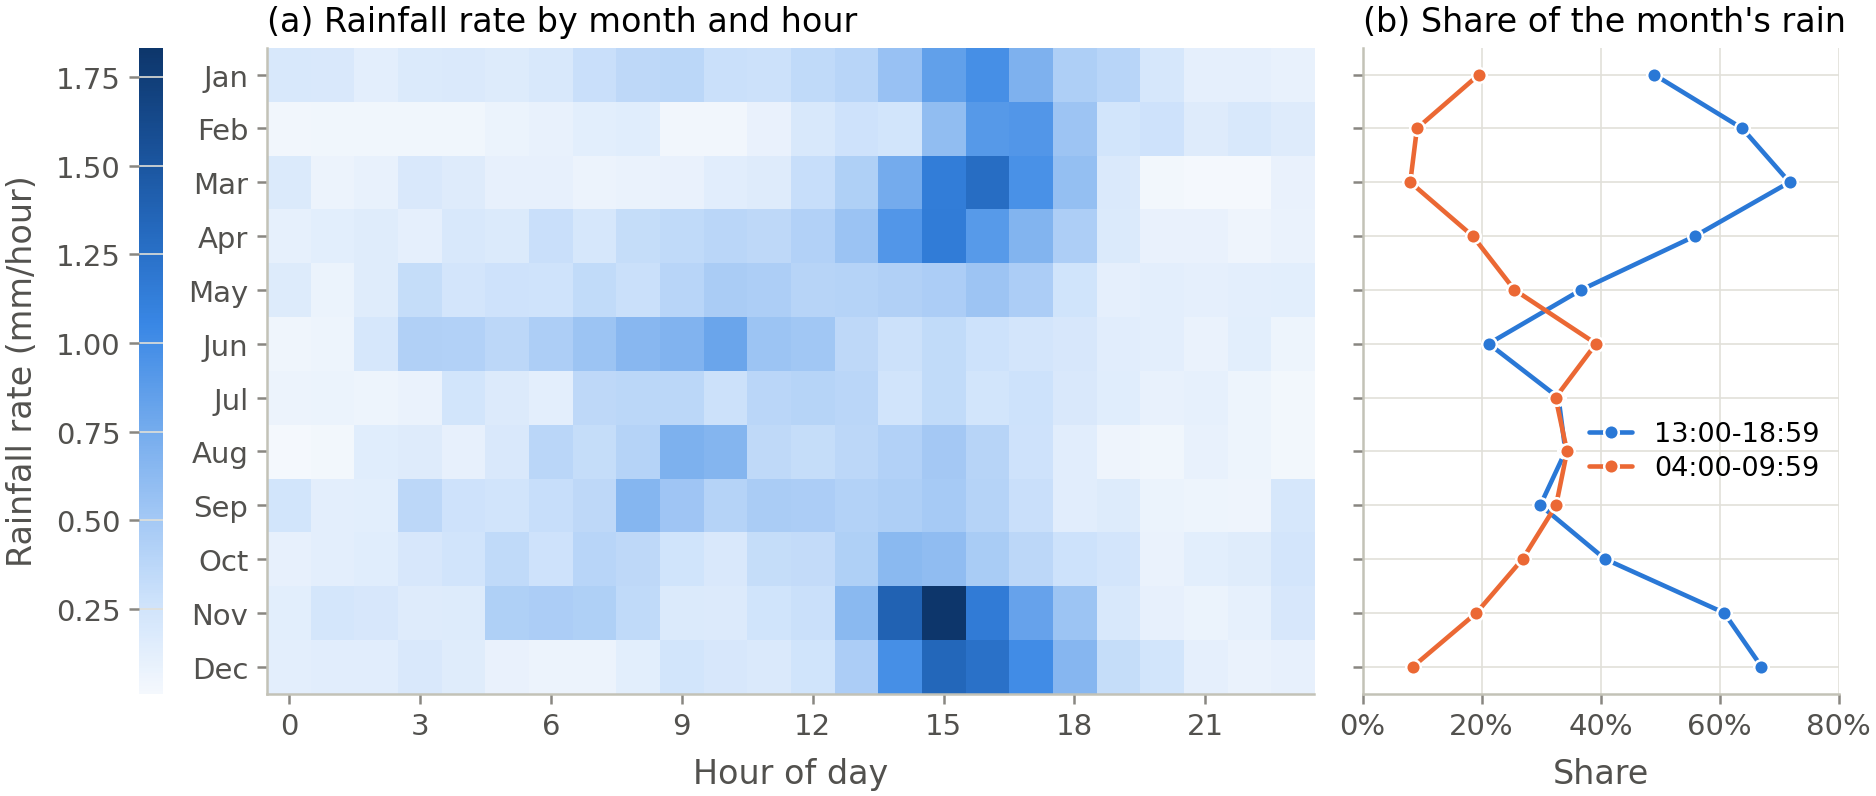
\includegraphics[width=0.96\linewidth,height=0.36\textheight,keepaspectratio]{figures/13_month_hour.png}
\caption{Timing of rain through the year, Singapore time. (a) Mean rainfall rate by month and hour of day; the colour scale is on the left. (b) Share of each month's rain that falls in the afternoon (13:00-18:59) and in the early morning (04:00-09:59). Early-morning rain peaks in June (\(39\%\) of that month's rain) against \(8\%\) in March, and in June, August and September the morning brings at least as much rain as the afternoon, consistent with the pre-dawn Sumatra squalls of the southwest monsoon.}
\label{fig:month-hour}
\end{figure}


\subsection*{4.5 Spatial Differences}
\phantomsection
\addcontentsline{toc}{subsection}{\numberline{4.5}Spatial Differences}


When examining rainfall patterns over the whole island, we hope to understand how it varies with location. Before implementing any formal tools, we aim to achieve a grouping of stations, which could help us build features that tell a station apart by the region it belongs to. To this end, we first gather stations that pass the \(90\%\) coverage check in a month and calculate their monthly rainfall rate. Then, we divided each rate by the network’s average of the same month to remove seasonality shared by all stations, and averaged the ratios over the station’s qualifying months. As a result, we found that the west of the island is clearly wetter than the rest. The discrepancy is significant, as the four wettest stations are all in the west with a relative level of 1.31 at Jurong West Street 73, and three of the four driest stations are in the east with 0.61 at Changi East Close in the far east.

\begin{figure}[!htbp]
\centering
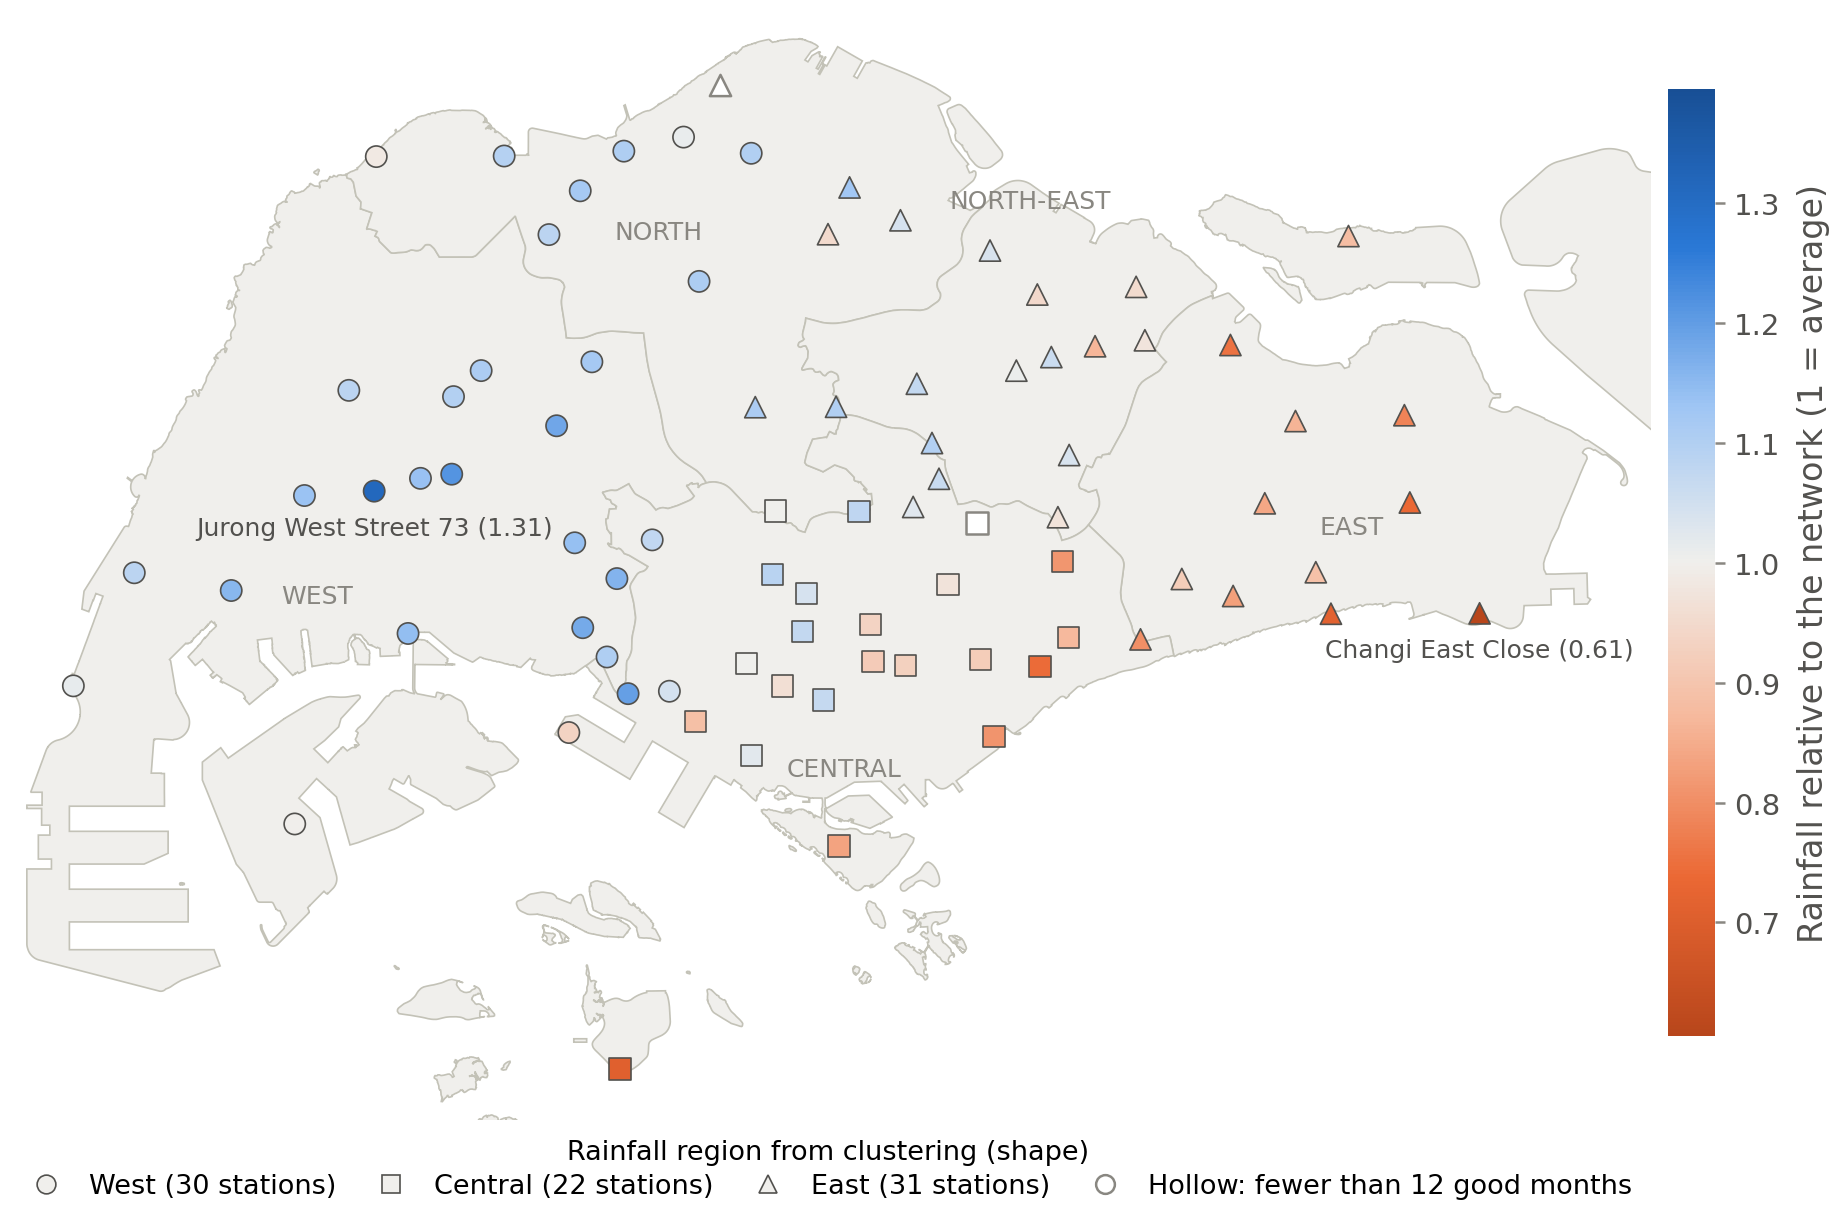
\includegraphics[width=0.94\linewidth,height=0.42\textheight,keepaspectratio]{figures/20_station_map.png}
\caption{Where it rains more, and which stations rain together. Colour: each station's rainfall rate relative to the whole network in the same months (station-months with at least \(90\%\) coverage, stations with at least 12 such months; \(1=\text{network average}\)), from 1.31 at Jurong West Street 73 to 0.61 at Changi East Close. Shape: rainfall regions found by Ward clustering of one minus the hourly correlation (69 stations with long overlapping records, 14 short-record stations assigned to the closest cluster); stations with too short a record for either measure (8) are not shown. Mean relative wetness is 1.11 in the West cluster, 0.94 in the Central cluster and 0.94 in the East cluster. Clusters built on odd years agree with those built on even years (adjusted Rand index~\citep{hubert1985} 0.78) and, in the held-out years, pairs in the same cluster correlate more than equally distant pairs in different clusters at \(3\text{--}8\,\mathrm{km}\) and \(8\text{--}13\,\mathrm{km}\) (one-sided Mann-Whitney \(p<0.05\)) but not further apart, so the regions are real but soft; agreement with the five official URA planning regions (grey outlines and labels) is 0.42. Station elevation is not in the dataset.}
\label{fig:station-map}
\end{figure}


We then group the stations by how they rain together and visualize it through different shapes in Figure~\ref{fig:station-map}. For every pair of stations, we correlated the hourly rainfall totals, kept the pairs that share at least about a yearly amount of hours, and finally clustered them with Ward’s method~\citep{ward1963} on one minus the correlation, dividing the whole network into three clusters, denoted as West, Central, and East. Referring to official planning regions~\citep{ura_regions}, we found that our clustering agrees largely with them. However, there are some exceptions; two stations are shown hollow because they belong to a cluster but did not pass the coverage check at the beginning, thus marked as hollow shapes.


Overall, our findings on the spatial distribution suggest two possible ways of feature encoding. First, a station can be described purely by its position and its typical wetness. We then encode the location as distances in kilometers east and north to the geographical center of the island, and add a station wetness ratio to reflect what we learned from the color pattern shown in Figure~\ref{fig:station-map}. Second, we clearly realized that rainfall at neighbouring stations should be informative. This is consistent with the regional nature of the rainy event and with our clustering result that stations in the same cluster rain together, yet are bounded within a finite enclosure. Regarding our lesson in this section, we will discuss further about how we built features from the recent rainfall of nearby stations in section 5.


\subsection*{4.6 Implications from clustering}
\phantomsection
\addcontentsline{toc}{subsection}{\numberline{4.6}Implications from clustering}


In section 4.5, the correlation of a station with its neighbours drew our attention, and it motivated our design of basic features such as the recent rainfall of nearby stations. However, the clustering that motivates this design lies on a single time scale, the hourly correlation. Namely, we have not yet understood how such correlation evolves in a larger spatial-temporal perspective. In order to quantify this, we generalize our correlation analysis to several distances and time windows. We first summed the five-minute readings into totals over 5 minutes, 15 minutes, 1 hour, etc. We then calculated the correlation of each pair of stations at each time scale and grouped them by distance, in bands of \(2\,\mathrm{km}\) up to \(10\,\mathrm{km}\). In Figure~\ref{fig:correlation-dynamics}, fitting these pairwise correlations with exponential decay suggest a clear decline of the correlation with distance. The decline is fast for short windows and slower for long ones, as within \(2\,\mathrm{km}\), the median correlation rises from 0.71 to 0.92. This then indicates that individual storms are local, consistent with the fact that whether the network is dry or wet is not uniform across the island, although a rainy day is island-wide. 


While leveraging the rainfall profile of neighbours brings no significant benefits in prediction, the virtue of such knowledge still lies in a different dimension; it potentially serves as a reliable proxy for filling up missing reading.                                        


\begin{figure}[!htbp]
\centering
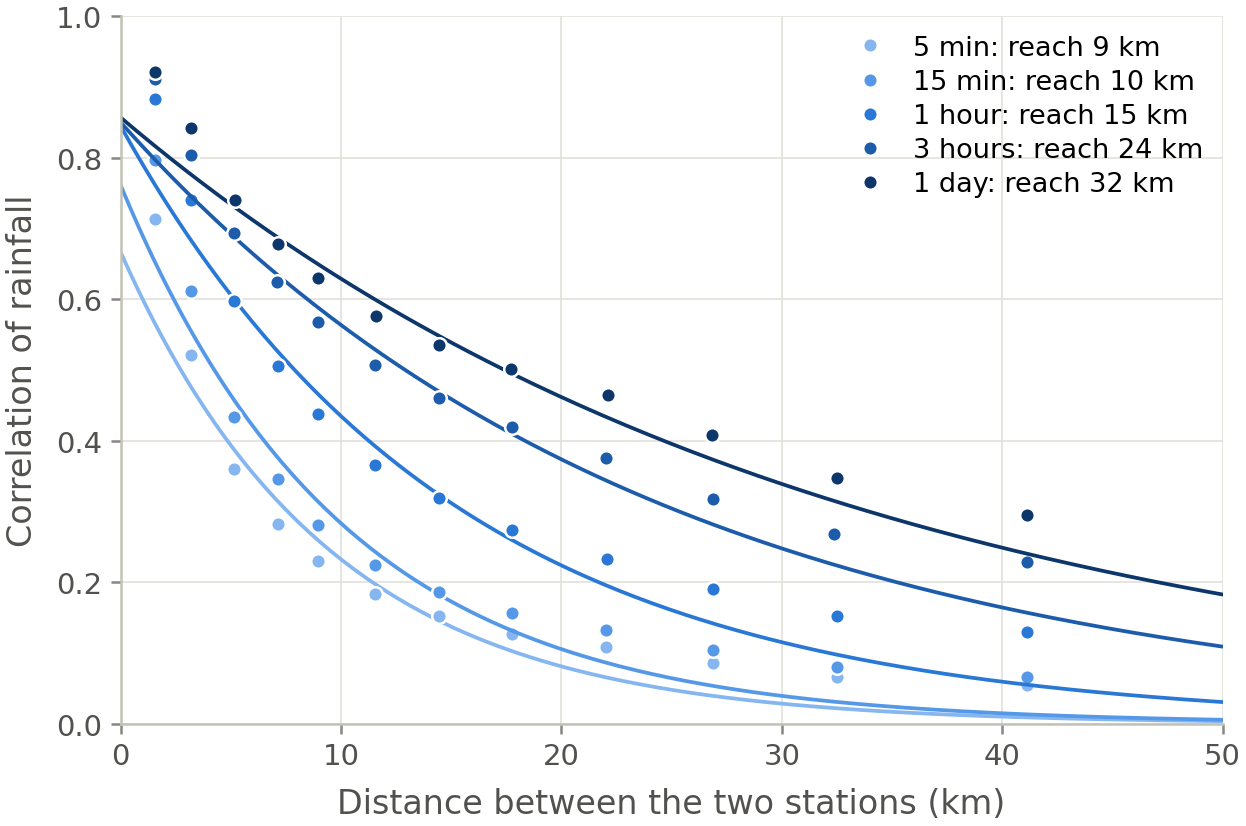
\includegraphics[width=0.84\linewidth,height=0.40\textheight,keepaspectratio]{figures/21_correlation_dynamics.png}
\caption{Correlation of rainfall between pairs of stations against their distance, for rain totals over five minutes to one day. Dots are medians per distance band; lines are fitted exponential decays \(c\exp\!\left(-\frac{d}{\mathrm{reach}}\right)\). The reach grows with the time window, from \(9\,\mathrm{km}\) for five-minute totals to \(32\,\mathrm{km}\) for daily totals, and within \(2\,\mathrm{km}\) the correlation rises from 0.71 to 0.92: individual storms are local, while rainy days are island-wide.}
\label{fig:correlation-dynamics}
\end{figure}


However, while our discussion above confirms the existence of neighbouring correlations, it does not yet explain why they differ between pairs of stations. The core issue is that a station’s correlation with its neighbours exists because of both convective, local rain and organized rain, such as monsoon squalls that cross the island systematically. Considering the geographical location of Singapore, it is plausible to draw an informative profile of the organized rain, since the seasonal monsoon makes the storms travel in particular, fixed directions. To estimate this, for every pair of stations 5 to \(30\,\mathrm{km}\) apart, we shifted one five-minute series against the other by up to 60 minutes before and after, and took the delay with the highest correlation. For example, rain at Kent Ridge Road is best matched by rain at Upper Serangoon Road, positioned roughly \(10\,\mathrm{km}\) away in its northeast direction, about a delay of 20 minutes that makes the correlation largest. We then regressed these best delays on the displacement between the two stations. To interpret this, note that the slope gives the direction and speed of the storms, and we listed out three typical groups of delays according to seasonality, including the Northeast monsoon, Southwest monsoon, and the inter-monsoon occurring during mid April and mid-October (Figure~\ref{fig:storm-motion}). Among three categories, the southwest monsoon shows the clearest picture (\(R^2=0.68\)) where the storms move east at about \(38\,\mathrm{km}\,\mathrm{h}^{-1}\). In short, the above findings motivated us to design features that capture changes in neighbouring rainfall profiles over past time windows while accounting for the seasonality of these effects.

\begin{figure}[!htbp]
\centering
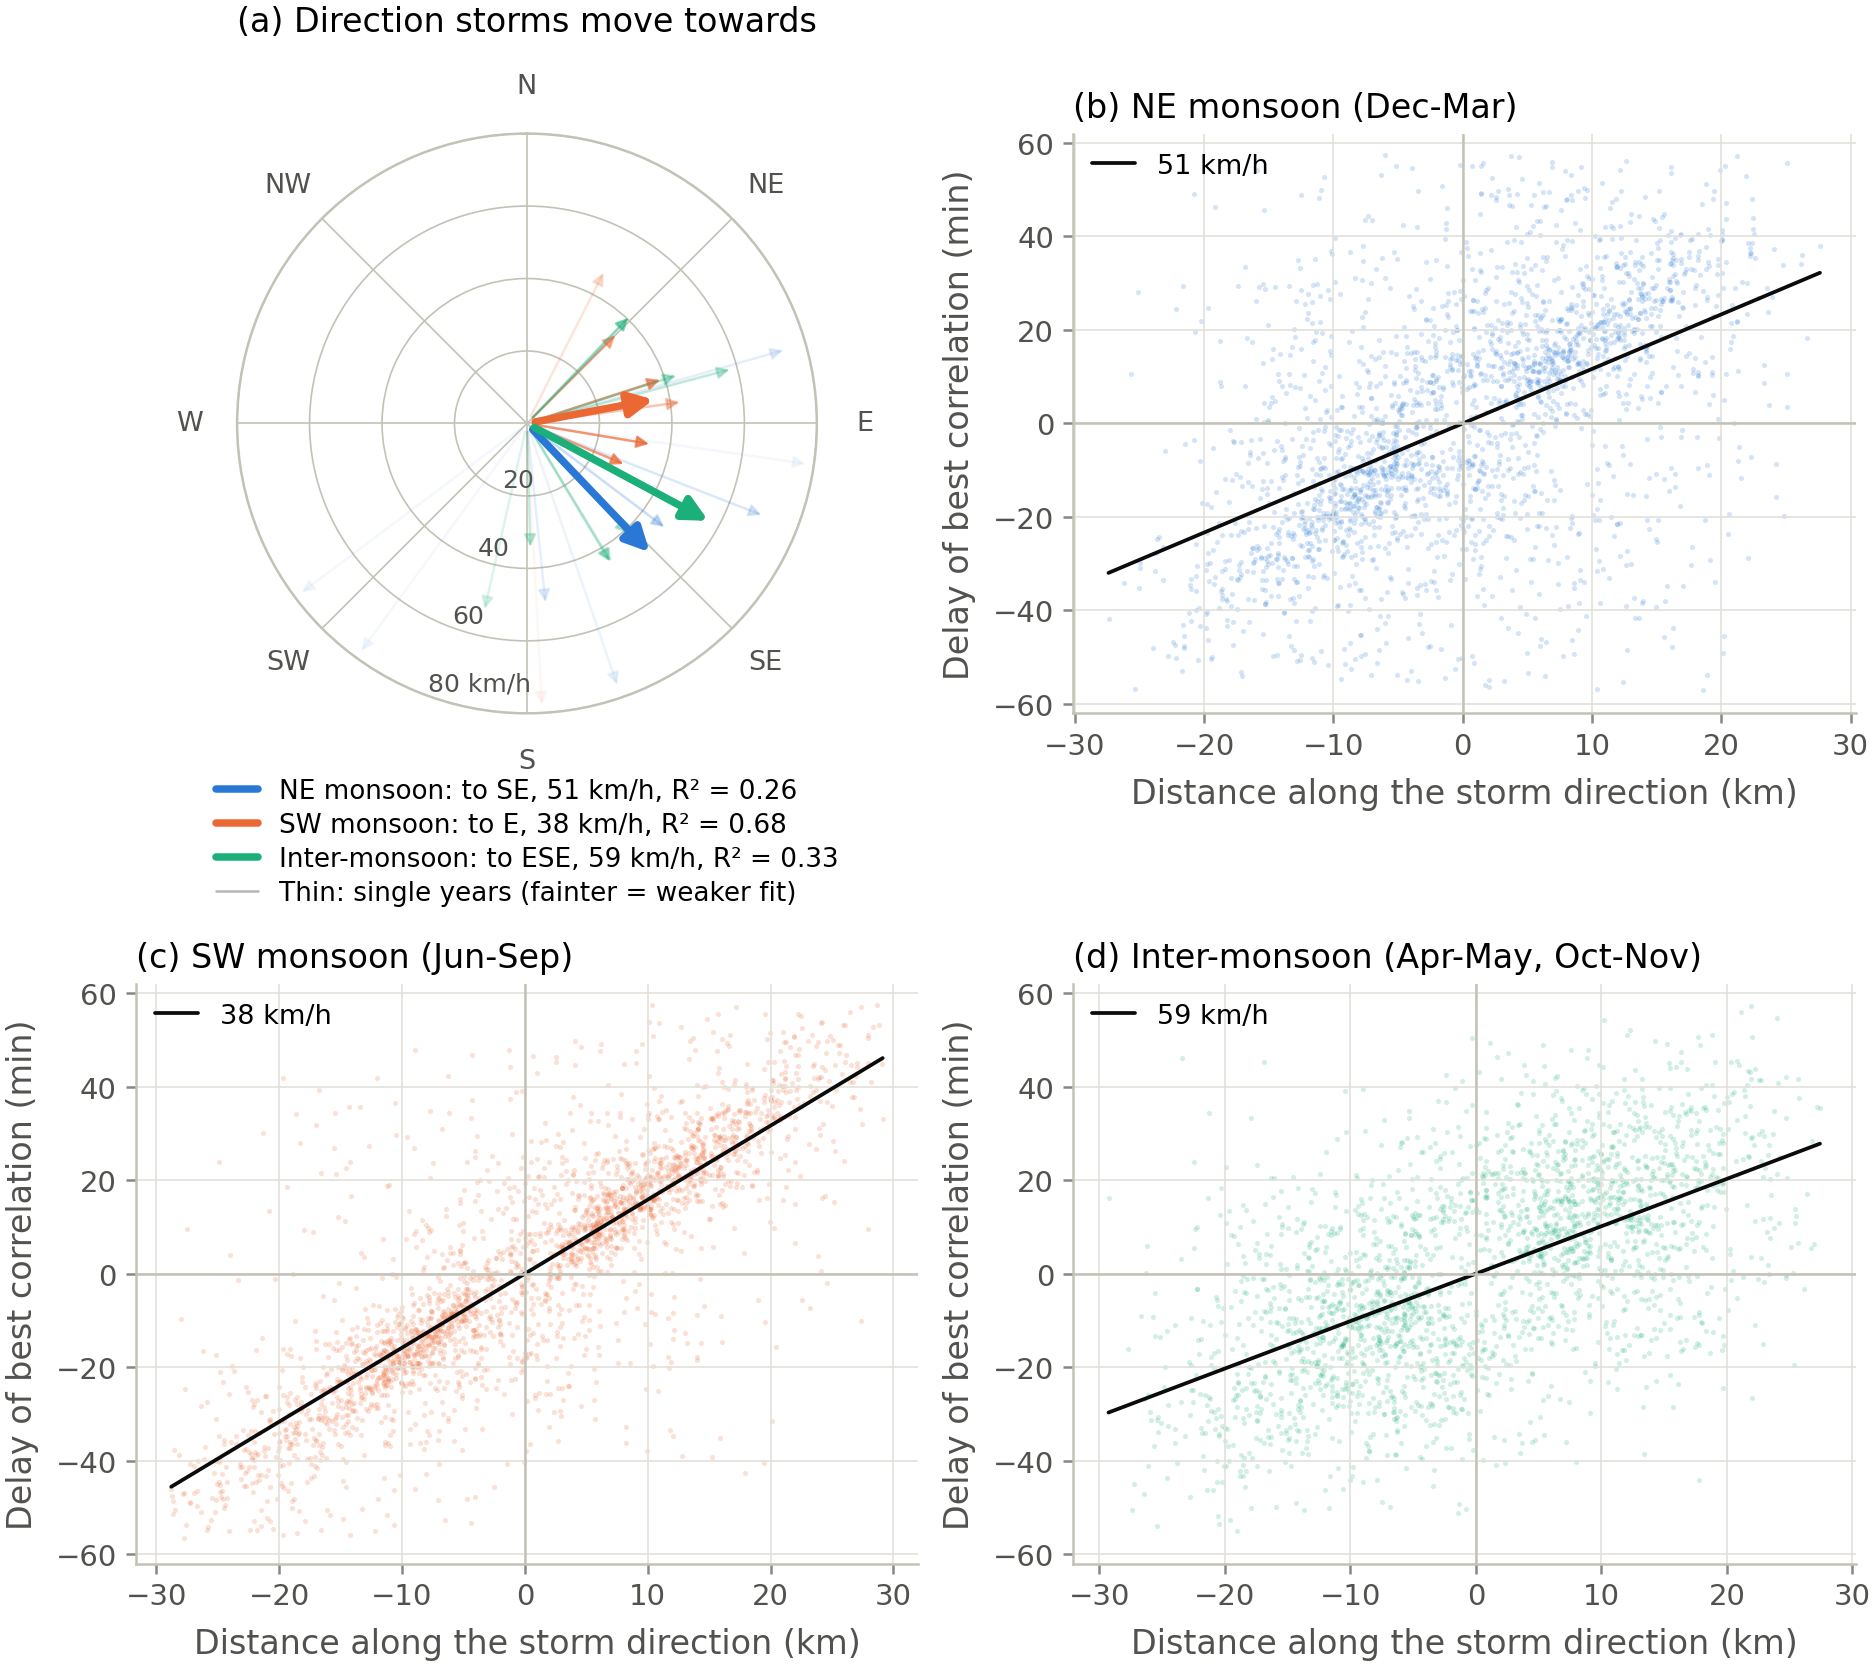
\includegraphics[width=0.92\linewidth,height=0.44\textheight,keepaspectratio]{figures/23_lead_lag.png}
\caption{Storm motion by monsoon season. For every station pair \(5\text{--}30\,\mathrm{km}\) apart, the five-minute series are shifted against each other by up to 60 minutes either way; the shift with the highest correlation is taken as the travel time, and a plane fit of travel time against the pairs' displacement gives the storm velocity. (a) Direction and speed of storm motion per season (thick arrows) and per single year (thin arrows, fainter for weaker fits). (b)-(d) Travel time against distance along the fitted direction; the line's slope is the inverse speed. In the southwest monsoon storms cross the island towards the east at about \(38\,\mathrm{km}\,\mathrm{h}^{-1}\) (\(R^2=0.68\)); in 6 of the 8 years the fit is clear (\(R^2\geq0.3\)), and all of these point between \(45^{\circ}\) and \(117^{\circ}\). The other seasons are less organised.}
\label{fig:storm-motion}
\end{figure}


\subsection*{4.7 Day-to-day persistence}
\phantomsection
\addcontentsline{toc}{subsection}{\numberline{4.7}Day-to-day persistence}


The preceding sections mainly examined station-specific rainfall profiles across seasonal cycles, various time scales, and neighbouring locations. However, these dimensions only describe how rainfall events unfold following prior, similar activities. Yet, we have been ignoring another critical aspect of forecasting future rainfall following a continuous dry period. This is exactly the most challenging part of the task, as predicting rainfall patterns from dry conditions requires modeling a near future that evolves under an uninformative context. To first quantify this problem, we plotted out the probability of observing a wet day (at least \(1\,\mathrm{mm}\) of precipitation) conditional on a wet/dry day preceding it. Based on daily totals, we pair every two consecutive days and categorize them based on precipitation level of the first day. From Figure~\ref{fig:daily-persistence}, we can tell that a clear discrepancy occurs in months such as  December, January, and February, where a wet day makes the next day much more likely to be wet, and vice versa. However, months like April and June barely show such two-day continuity. We claim that the seasonal cycle partly explains such a gap between months. In December to March, when the northeast monsoon is prevalent, the direction in which storms move between stations is the least organized (\(R^2=0.26\)), creating a more chaotic, slower system that lasts for more than a day and tends to make two-day precipitation alike. On the contrary, in the southwest monsoon, storms move in a clearer direction, thus making the next day more independent than its preceding one. However, such conclusions are not fully supported by analytical integrity or statistical significance; yet, they offer a reasonable foundation to understand how different precipitation factors may interact in an non-linear manner.

\begin{figure}[!htbp]
\centering
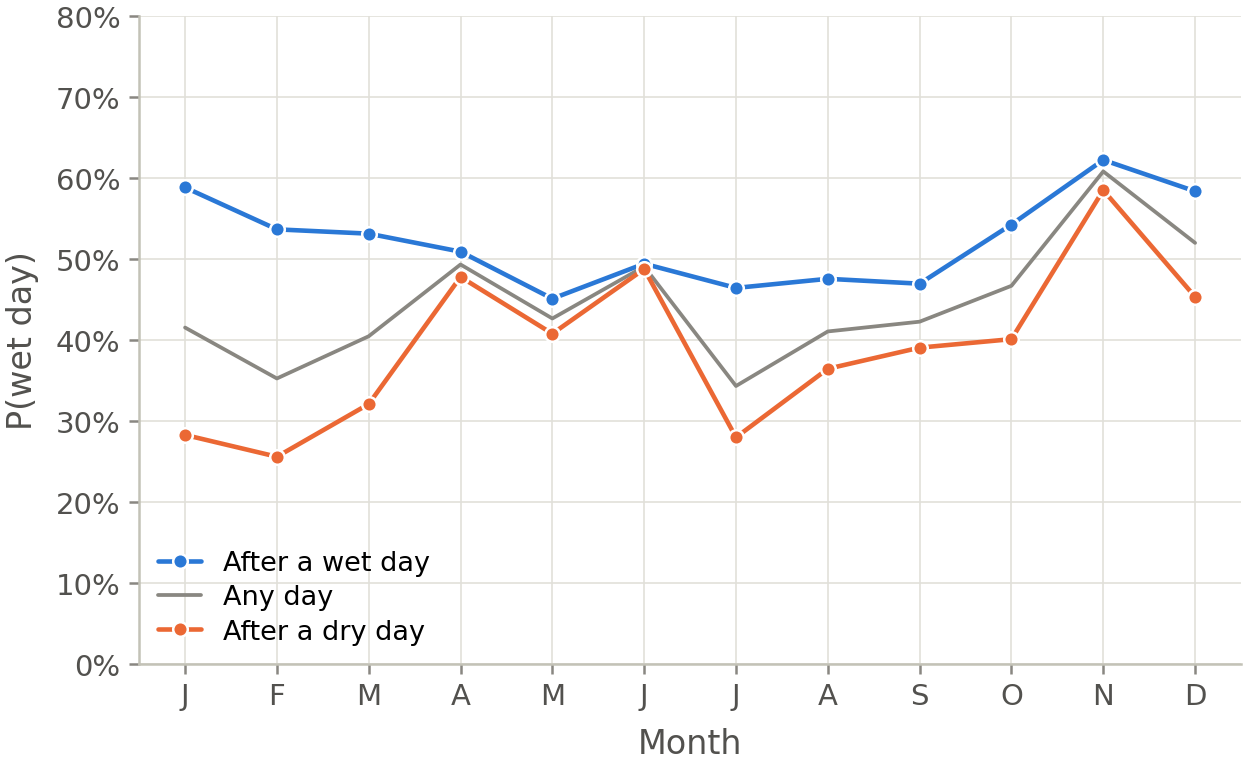
\includegraphics[width=0.84\linewidth,height=0.36\textheight,keepaspectratio]{figures/31_persistence.png}
\caption{Day-to-day persistence of rain. Probability that a station-day is wet (at least \(1\,\mathrm{mm}\)) after a wet day (blue), after a dry day (orange) and on any day (grey), by month; only complete days are used. Over the year a wet day follows a wet day \(53\%\) of the time and a dry day \(38\%\) of the time. The gap is widest in January (\(59\%\) against \(28\%\)) and almost vanishes in June (\(49\%\) against \(49\%\)), consistent with the short-lived storms of the southwest monsoon.}
\label{fig:daily-persistence}
\end{figure}


\subsection*{4.8 Implications for prediction}
\phantomsection
\addcontentsline{toc}{subsection}{\numberline{4.8}Implications for prediction}


To date, we have made attempts to explore from different dimensions how historical precipitation profiling can inform a near-future event. These perspectives include, but are not limited to, the static properties of a station (longitude, latitude), inherent cyclic patterns (monthly and diurnal dynamics), neighbourhood effects (the informative history of adjacent stations), and island-wide rainfall dynamics (monsoonal patterns). Levering these insights, we now discuss how these findings can be translated into predictive features, with a primary focus on the feature-engineering process. In short, the evidence translates into six design principles; each will be discussed below, while their exact construction is given in section 5.3.


To connect findings to features, we start with the static context. As discussed in 4.2 and 4.3, the seasonal effects are real but modest statistically, and differences between years are small. Hence, we encode the time of year with sine/cosine terms and the monsoon indicator (discussed in 4.6), instead of identifying an exact year. Then, we found in section 4.4 that the afternoon peak comes mainly from more frequent rain and its timing shifts with the season, so we encode the hour cyclically and let it interact with the season. Finally, section 4.5 suggests that the west of the island is typically wetter and the divisions of precipitation profiles are soft. Based on this observation, we will describe a station by its position and its typical wetness instead of hard regional labeling. 


Second, we consider the recent rainfall history of a station. We learned that clearly, the recent rain at a station is informative and day-to-day continuity exists yet depends on the season. We therefore give the model rain over several past windows, acknowledging the virtue of historical profiling.


On top of that, we summarize nearby stations by distance and direction (north, east, south, and west) as directed by section 4.6. 


To zoom out from local rainfall events, we also looked at island-wide dynamics and found that organized storms move in seasonal directions, most clearly in the southwest monsoon (section 4.6). Hence, we add one more layer to the above features, the exact upstream rainfall and the change in the neighbours’ rainfall. 


\FloatBarrier

\section*{5. Task 2: Prediction Methodology}
\phantomsection
\addcontentsline{toc}{section}{\numberline{5.}Task 2: Prediction Methodology}


We estimate the probability that station rainfall will exceed a user-specified threshold over the next 30 minutes. A nine-class rainfall distribution is predicted from recent observations and spatial summaries, then converted into threshold exceedance probabilities. The final random forest achieves an RPS of 0.0887 on 2024, compared with 0.1246 for probabilistic persistence. Section 5.4 explains a qualification concerning the estimation period of the storm-motion prior. 


\subsection*{5.1 Prediction Target and Information Available at Forecast Time}
\phantomsection
\addcontentsline{toc}{subsection}{\numberline{5.1}Prediction Target and Information Available at Forecast Time}


For station \(s\) and prediction slot \(t\), let \(r_{s,t}\) denote the recorded rainfall in a five-minute slot. We define the response as the total over the next six slots:


\[
Y_{s,t}=\sum_{k=1}^{6}r_{s,t+k}
\]


\[
p_{s,t}(\theta)=P(Y_{s,t}>\theta\mid x_{s,t}),\qquad\theta\geq0.
\]


The input vector \(x_{s,t}\) describes station \(s\) at forecast time \(t\). It contains 58 features from the four tiers introduced in Section 5.3. Each row is therefore one forecast for one station and one five-minute time slot. The station ID and timestamp are used to join the data, while station position and calendar variables enter the model as features. The future rainfall total and its class label are used as the response, not as input features.


The current reading belongs to the information set, while the response starts at the following slot. Forecasts therefore concern accumulated rainfall during the next 30 minutes. A pooled model is fitted across stations, with station attributes and neighbourhood summaries accounting for spatial differences.


At prediction time, the inputs comprise rainfall at the target station and other reporting stations up to and including \(t\), station coordinates, calendar variables and previously estimated station statistics. No temperature, humidity, radar or numerical weather forecast is used. We assume that all readings timestamped \(t\) are available when the forecast is issued; ingestion delays are not simulated. The seasonal storm-motion constants are fixed before each prediction, although their estimation period creates the qualification discussed in Section 5.4. 


\subsection*{5.2 Label Construction and Probability Representation}
\phantomsection
\addcontentsline{toc}{subsection}{\numberline{5.2}Label Construction and Probability Representation}


\subsubsection*{Cleaning and eligible samples}
\phantomsection
\addcontentsline{toc}{subsubsection}{Cleaning and eligible samples}


The input is the aligned five-minute rainfall matrix produced in Task 1. Missing readings remain missing. Before constructing labels or rainfall features, we mask suspected stuck-gauge months: a station-month is flagged when it has no wet readings despite at least 30 expected wet readings under the contemporaneous network wet frequency. This identifies 18 station-months. We also mask two identified faulty periods, S107 from 19 August 2022 at 22:00 to 22 August 2022 at 06:00, and S36 from 1 February 2019 to 1 September 2021; end times are excluded.


A row is retained only when the current reading and all six future readings exist and the future window ends in the same calendar year. This prevents the response window from crossing a training, validation or test boundary. The future total is rounded to \(0.1\,\mathrm{mm}\) to remove floating-point noise. The resulting dataset contains 47,511,766 labelled station-slot observations; \(93.84\%\) have no rain in the next 30 minutes.


\subsubsection*{Nine rainfall classes}
\phantomsection
\addcontentsline{toc}{subsubsection}{Nine rainfall classes}


We discretise the response into nine ordered classes, retaining a separate point mass at zero and progressively wider intervals for heavier rainfall. Both learning algorithms predict the complete vector of class probabilities, \(p_k(x)=P(C=k\mid x)\), whose components sum to one. 


We keep zero rainfall as a separate class because dry windows make up most of the data. The lower rainfall ranges are divided more finely, while wider intervals are used for heavier rainfall, where observations are less frequent. This gives the models more detail near the dry-to-wet boundary without dividing the rare heavy-rainfall cases into many small groups. These cutoffs are a design choice; we do not claim that nine classes are the best possible division.


\Needspace{4\baselineskip}
\begingroup
\small
\setlength{\parskip}{0pt}
\renewcommand{\arraystretch}{1.18}
\begin{longtable}{@{}>{\raggedright\arraybackslash}p{(\linewidth-6\tabcolsep)*\real{0.12}}>{\raggedright\arraybackslash}p{(\linewidth-6\tabcolsep)*\real{0.38}}>{\raggedright\arraybackslash}p{(\linewidth-6\tabcolsep)*\real{0.12}}>{\raggedright\arraybackslash}p{(\linewidth-6\tabcolsep)*\real{0.38}}@{}}
\caption*{\textbf{Table 5.1.} Rainfall classes for the next 30 minutes}\\
\toprule
\textbf{Class} & \textbf{Rainfall total in mm} & \textbf{Class} & \textbf{Rainfall total in mm} \\
\midrule
\endfirsthead
\toprule
\textbf{Class} & \textbf{Rainfall total in mm} & \textbf{Class} & \textbf{Rainfall total in mm} \\
\midrule
\endhead
0 & \(Y=0\) & 5 & \(2<Y\leq5\) \\
1 & \(0<Y\leq0.2\) & 6 & \(5<Y\leq10\) \\
2 & \(0.2<Y\leq0.5\) & 7 & \(10<Y\leq20\) \\
3 & \(0.5<Y\leq1\) & 8 & \(Y>20\) \\
4 & \(1<Y\leq2\) &  &  \\
\bottomrule
\end{longtable}
\endgroup


The implementation places each split \(0.05\,\mathrm{mm}\) above its stated edge, for example 0.25 for the \(0.2\,\mathrm{mm}\) boundary. On the rounded response grid, this keeps a value exactly at an edge in the lower class. 


\subsubsection*{Mapping class probabilities to any threshold}
\phantomsection
\addcontentsline{toc}{subsubsection}{Mapping class probabilities to any threshold}


At a class boundary, the exceedance probability is obtained by adding the probabilities of all higher classes. A threshold inside a class needs one extra step. For example, the class \(2<Y\leq 5\) contains rainfall amounts both below and above \(3\,\mathrm{mm}\). The model gives a probability for this whole class, so we use the fitting data to estimate the fraction that lies above \(3\,\mathrm{mm}\). 


For a threshold \(\theta\) inside wet class \(k\), this fraction is


\[
\widehat q_k(\theta)=\frac{\sum_{i\in\mathcal D_{\mathrm{fit}}} w_i\,\mathbf{1}(C_i=k)\,\mathbf{1}(Y_i>\theta)}{\sum_{i\in\mathcal D_{\mathrm{fit}}} w_i\,\mathbf{1}(C_i=k)}
\]


Here, \(\mathcal D_{\mathrm{fit}}\) is the data used to fit the mapper, \(C_i\) is the rainfall class, and \(w_i\) is the row weight. All weights are one in the final full-data fit. The mapper uses 2017–2022 for validation experiments and 2017–2023 for final test scoring.


The class probability changes with the input, but the fraction \(\widehat q_k(\theta)\) is shared across inputs. For example, if \(40\%\) of fitting observations in class 5 exceed \(3\,\mathrm{mm}\), we use \(0.4p_5(x)\) from that class, together with all probabilities from classes 6 to 8. The mapper is fitted once and saved with the model; it does not use the future rainfall of the observation being predicted.


The exceedance probability is then:


\[
\widehat P(Y>\theta\mid x)=\sum_{j=k+1}^{8}p_j(x)+p_k(x)\widehat q_k(\theta).
\]


This construction gives coherent, non-increasing exceedance probabilities across thresholds. Within each class, however, the empirical rainfall distribution is shared across inputs. Its tail is bounded by the largest observed fitting value, \(71.8\,\mathrm{mm}\) in the saved final mapper, so it cannot extrapolate beyond that amount. 


\subsection*{5.3 Feature Engineering}
\phantomsection
\addcontentsline{toc}{subsection}{\numberline{5.3}Feature Engineering}


The final feature set contains 58 original columns organised into four tiers. This organisation separates station and calendar effects from local rainfall history, surrounding rainfall and changes in that surrounding rainfall. All dynamic features use observations at \(t\) or earlier. The dimension passed to logistic regression increases after encoding and feature expansion.


\Needspace{4\baselineskip}
\begingroup
\small
\setlength{\parskip}{0pt}
\renewcommand{\arraystretch}{1.18}
\begin{longtable}{@{}>{\raggedright\arraybackslash}p{(\linewidth-4\tabcolsep)*\real{0.09}}>{\raggedright\arraybackslash}p{(\linewidth-4\tabcolsep)*\real{0.12}}>{\raggedright\arraybackslash}p{(\linewidth-4\tabcolsep)*\real{0.79}}@{}}
\caption*{\textbf{Table 5.2.} Feature groups and their purposes}\\
\toprule
\textbf{Tier} & \textbf{Columns} & \textbf{Contents} \\
\midrule
\endfirsthead
\toprule
\textbf{Tier} & \textbf{Columns} & \textbf{Contents} \\
\midrule
\endhead
T0 & 15 & Station position and wetness ratios; daily and annual harmonics; monsoon season \\
T1 & 11 & Recent rainfall totals, maximum intensity, wet slots, trend, time since rain and missingness \\
T2 & 15 & Neighbour rainfall by distance and direction, wet fractions, nearest rain and network conditions \\
T3 & 17 & Changes in 12 spatial summaries, four upstream summaries and upstream station coverage \\
\bottomrule
\end{longtable}
\endgroup


\subsubsection*{Tier 0 station and calendar information}
\phantomsection
\addcontentsline{toc}{subsubsection}{Tier 0 station and calendar information}


Longitude and latitude are projected onto a local kilometre grid centred at \(103.82^{\circ}\) E and \(1.35^{\circ}\) N. Two additional station attributes compare observed wet and heavy-rain windows with the number expected from the network at the same slots. Heavy rain here means \(Y>5\,\mathrm{mm}\). 


To calculate a station's wetness ratio, we compare its observed number of wet future windows with the number expected from the network at the same times. For each slot, we calculate the fraction of stations with a valid label whose next 30 minutes are wet. We then sum these fractions over the training slots available at the target station. Comparing the same times reduces the effect of stations reporting in different years or seasons. 


Writing the observed and expected counts as \(O_s\) and \(E_s\), the station feature is


\[
\mathrm{wet\_ratio}_s=\frac{O_s+500}{E_s+500}
\]


A ratio above one indicates more wet windows than expected. Adding 500 pulls estimates towards one when the record is short. The heavy-rainfall ratio is calculated in the same way using \(Y>5\,\mathrm{mm}\). Both features are estimated from 2017–2022 labels and kept fixed afterwards. 


Time of day is represented by three sine/cosine harmonic pairs, and time of year by two pairs, accounting for leap years. A monsoon code distinguishes December–March, June–September and the intervening months. Cyclic encoding keeps adjacent dates and hours close at the boundaries of a day or year. 


\subsubsection*{Tier 1 rainfall at the target station}
\phantomsection
\addcontentsline{toc}{subsubsection}{Tier 1 rainfall at the target station}


Six totals summarise the last 5, 15, 30, 60, 120 and 1,440 minutes, including the current reading. The remaining features are the largest five-minute amount in the last 30 minutes, the number of wet slots in the last hour, the change between successive 15-minute totals, minutes since the last wet reading capped at 1,440, and missing readings in the last two hours. 


Let \(R_{s,t}^{(L)}\) denote rainfall over the last \(L\) minutes. Since each slot lasts five minutes, this uses slots \(t-\frac{L}{5}+1\) through \(t\). For example, at 16:00, the 15-minute feature adds the readings at 15:50, 15:55 and 16:00. The response uses the next six readings, from 16:05 to 16:30.


\[
\mathrm{trend}_{s,t}=R_{s,t}^{(15)}-\bigl(R_{s,t}^{(30)}-R_{s,t}^{(15)}\bigr)=2R_{s,t}^{(15)}-R_{s,t}^{(30)}.
\]


If the last 15 and 30 minutes contain 1.8 and \(3.2\,\mathrm{mm}\), the trend is \(0.4\,\mathrm{mm}\): the most recent 15 minutes contain \(1.8\,\mathrm{mm}\) and the preceding 15 minutes contain \(1.4\,\mathrm{mm}\). A positive value therefore indicates increasing recent rainfall.


Rolling calculations skip missing readings rather than imputing them as dry observations. Consequently, a sum may cover less than its nominal window; the missingness feature gives the model an indication of this loss of coverage. Features are calculated on the complete grid before rows without a current observation are removed.


\subsubsection*{Tier 2 rainfall at other stations}
\phantomsection
\addcontentsline{toc}{subsubsection}{Tier 2 rainfall at other stations}


Tier 2 summarises the spatial rainfall field. Within \(10\,\mathrm{km}\), rainfall totals over 15 and 30 minutes use inverse squared distance weights, with a \(0.5\,\mathrm{km}\) distance floor. A second weighted mean covers the \(10\text{--}25\,\mathrm{km}\) ring. Other features include the largest nearby 30-minute total, wet-station shares within 5 and \(10\,\mathrm{km}\), distance to the nearest station wet in the last 15 minutes capped at \(30\,\mathrm{km}\), and mean 30-minute rainfall in four compass quadrants within \(25\,\mathrm{km}\).


Let \(d_{sj}\) be the distance in kilometres between target station \(s\) and neighbour \(j\), and let \(a_{j,t}=1\) when station \(j\) reports at time \(t\). The nearby rainfall weight is


\[
w_{sj}=\frac{\mathbf{1}(0<d_{sj}\leq10)}{\max(d_{sj},0.5)^2}
\]


The 15-minute neighbour rainfall feature is


\[
\mathrm{IDW}_{s,t}^{(15)}=\frac{\sum_j w_{sj}\,a_{j,t}\,R_{j,t}^{(15)}}{\sum_j w_{sj}\,a_{j,t}}
\]


The same calculation is used for the 30-minute total. A station \(2\,\mathrm{km}\) away has four times the weight of one \(4\,\mathrm{km}\) away. The spatial wet fractions use any rainfall in the preceding 30 minutes, while the nearest-rain distance uses the preceding 15 minutes. These summaries can provide information about rain before it is observed at the target station. 


Two network summaries describe the island-wide mean rainfall and wet-station share. A count of reporting neighbours within \(10\,\mathrm{km}\) indicates local coverage. Local neighbourhood features exclude the target station; the network summaries include it. Weighted averages are normalised over currently reporting stations, so a missing neighbour does not dilute the denominator. A summary with no available neighbour is set to zero. The station count helps distinguish limited coverage from genuinely dry conditions, although it does not fully describe coverage for every region.


\subsubsection*{Tier3 neighborhood change and upstream rainfall}
\phantomsection
\addcontentsline{toc}{subsubsection}{Tier3 neighborhood change and upstream rainfall}


Tier 3 adds the 15-minute changes in twelve selected Tier 2 summaries. For a summary \(F\), the change is


\[
\Delta F_{s,t}=F_{s,t}-F_{s,t-3}
\]


The earlier value is recomputed from the network readings at \(t-3\), so it does not require the target station to have reported then. A positive change in neighbour rainfall indicates that surrounding rain has increased. A negative change in nearest-rain distance means the nearest observed rain is closer, although it does not establish that the same storm has moved towards the station.


Four upstream features follow the seasonal average storm motion backwards from the target station to locations corresponding to 15 and 30 minutes of travel. Around each location, a Gaussian kernel with a standard deviation of \(4\,\mathrm{km}\) and a radius of \(10\,\mathrm{km}\) summarises the latest 15-minute rainfall and wet-station share. A fifth feature counts reporting stations around the 30-minute upstream point. This matters near coasts, where the upstream point may lie outside the gauge network. The fixed seasonal headings and speeds are listed below.


Let \(z_s=(x_s,y_s)\) be the station position, \(v_\sigma\) the seasonal speed in \(\mathrm{km}\,\mathrm{h}^{-1}\), and \(\varphi_\sigma\) the heading towards which rain moves, measured clockwise from north. The upstream position for a travel time of \(\tau\) minutes is


\[
u_{s,\tau}=z_s-v_\sigma\frac{\tau}{60}\begin{pmatrix}\sin(\varphi_\sigma)\\\cos(\varphi_\sigma)\end{pmatrix},\qquad\tau\in\{15,30\}.
\]


For example, a speed of about \(38\,\mathrm{km}\,\mathrm{h}^{-1}\) gives a 15-minute upstream distance of about \(9.5\,\mathrm{km}\). This is a fixed seasonal estimate of where incoming rain may be found. It does not track the current storm, and the upstream averages exclude the target station.


\Needspace{4\baselineskip}
\begingroup
\small
\setlength{\parskip}{0pt}
\renewcommand{\arraystretch}{1.18}
\begin{longtable}{@{}>{\raggedright\arraybackslash}p{(\linewidth-4\tabcolsep)*\real{0.38}}>{\raggedright\arraybackslash}p{(\linewidth-4\tabcolsep)*\real{0.34}}>{\raggedright\arraybackslash}p{(\linewidth-4\tabcolsep)*\real{0.28}}@{}}
\caption*{\textbf{Table 5.3.} Seasonal motion parameters used for the upstream kernels}\\
\toprule
\textbf{Season} & \textbf{Heading towards} & \textbf{Speed in \(\mathrm{km}\,\mathrm{h}^{-1}\)} \\
\midrule
\endfirsthead
\toprule
\textbf{Season} & \textbf{Heading towards} & \textbf{Speed in \(\mathrm{km}\,\mathrm{h}^{-1}\)} \\
\midrule
\endhead
NE monsoon & \(136.4^{\circ}\)  & 51.4 \\
Inter-monsoon & \(118.2^{\circ}\)  & 59.1 \\
SW monsoon & \(79.3^{\circ}\)  & 37.9 \\
\bottomrule
\end{longtable}
\endgroup


Heading is clockwise from north. These parameters describe an average statistical propagation pattern, rather than a real-time track of each storm. 


\subsection*{5.4 Training, Validation, and Test Design}
\phantomsection
\addcontentsline{toc}{subsection}{\numberline{5.4}Training, Validation, and Test Design}


We use a chronological split to evaluate forecasts on later years. All stations share the same temporal boundaries. Randomly splitting rows would place closely spaced, overlapping rainfall windows in different subsets and would not reflect forecasting a future period.


\Needspace{4\baselineskip}
\begingroup
\small
\setlength{\parskip}{0pt}
\renewcommand{\arraystretch}{1.18}
\begin{longtable}{@{}>{\raggedright\arraybackslash}p{(\linewidth-6\tabcolsep)*\real{0.18}}>{\raggedright\arraybackslash}p{(\linewidth-6\tabcolsep)*\real{0.18}}>{\raggedright\arraybackslash}p{(\linewidth-6\tabcolsep)*\real{0.19}}>{\raggedright\arraybackslash}p{(\linewidth-6\tabcolsep)*\real{0.45}}@{}}
\caption*{\textbf{Table 5.4.} Chronological data partitions}\\
\toprule
\textbf{Partition} & \textbf{Years} & \textbf{Rows} & \textbf{Purpose} \\
\midrule
\endfirsthead
\toprule
\textbf{Partition} & \textbf{Years} & \textbf{Rows} & \textbf{Purpose} \\
\midrule
\endhead
Training & 2017-2022 & 34418016 & Initial model fitting \\
Validation & 2023 & 6719274 & Configuration (Hyperparameter) selection \\
Final fitting & 2017-2023 & 41137290 & Full data after configuration selection \\
Test & 2024 & 6374476 & Final scoring \\
\bottomrule
\end{longtable}
\endgroup


Candidate models are fitted on 2017–2022, and their settings are selected using RPS on the 2023 validation data. Once the settings are fixed, both LR and RF are fitted again on the full 2017–2023 dataset using all four feature tiers. This final fitting table contains 41,137,290 rows, with weight one for every row. The 2024 data are then used for final scoring.


The final LR fit had already completed before the remote connection was interrupted. When the run resumed, the saved LR pipeline was loaded instead of repeating that completed fit. The mapper and baselines are also fitted on 2017–2023. Station wetness ratios remain fixed at their 2017–2022 values, while LR scaling parameters are learned from the data used for the corresponding fit.


The final experiment uses the full dataset. For smaller machines, an optional development table retains every wet row and samples dry rows with probability \(f=0.1\). Each retained dry row receives weight \(\frac{1}{f}=10\), while each wet row receives weight one. This corrects for the different sampling probabilities. Validation and test data are never subsampled. This option is separate from the RF row subsampling rate of 0.5, which controls sampling for each tree within the forest.


The implementation uses Spark window operations for temporal features, Parquet for intermediate tables and Spark ML pipelines for fitting. Spatial summaries pivot stations into a vector for each slot and use batched NumPy matrix operations through mapInPandas. The final run used a remote compute node with 32 vCPUs and approximately 256 GB of RAM. Spark is configured in local mode on the remote node; no multi-node scaling benchmark is reported. 


\subsubsection*{Qualification concerning the motion prior}
\phantomsection
\addcontentsline{toc}{subsubsection}{Qualification concerning the motion prior}


The Task 1 matrix builder covers 2017–2024. Its load\_matrix routine concatenates all year partitions, and lead\_lag estimates seasonal motion on the pooled matrix without restricting the fitting years. Since Tier 3 imports the motion estimates attributed to that analysis, its upstream prior uses information from the validation and test periods. The classifier fitting and response construction retain their chronological split, but the complete feature-design procedure is not independent of 2024. The reported scores describe this implementation and should not be presented as a fully untouched prospective test. A stricter experiment would estimate motion using 2017–2022 for validation and freeze or re-estimate it using years through 2023 before evaluating 2024.


\subsection*{5.5 Baseline Models}
\phantomsection
\addcontentsline{toc}{subsection}{\numberline{5.5}Baseline Models}


All baselines output the same nine-class probability vector as the learning models and are evaluated with the same scoring functions. For validation, the climatology and persistence tables are estimated from all 2017–2022 labels. For test scoring, the baselines are refitted on the full 2017–2023 fitting table.


The constant baseline uses the class frequencies in the fitting data and gives the same probability vector to every observation.


Climatology uses the station, calendar month and hour. Its class frequencies are pulled towards the network frequencies for the same month and hour:


\[
\widehat p_k(s,m,h)=\frac{n_{s,m,h,k}+M q_{m,h,k}}{n_{s,m,h}+M}
\]


Here, \(n_{s,m,h,k}\) is the fitted count for class \(k\), \(n_{s,m,h}\) is the total count for that station-month-hour group, and \(q_{m,h,k}\) is the network class frequency for the same month and hour. The parameter \(M\) controls how much the station estimate is pulled towards the network estimate. A group with fewer observations receives more shrinkage. If no station-specific estimate is available, we use the network frequencies. We compare shrinkage strengths 0, 100, 1,000, 3,000 and 10,000 on 2023; the selected value is 3,000. Groups without station-specific estimates fall back to the network distribution.


Probabilistic persistence uses the rainfall class of the previous 30 minutes. From the fitting data, it estimates


\[
P(C_{\mathrm{future}}=k\mid C_{\mathrm{past}}=j)
\]


It therefore predicts a distribution of future classes for each past class, rather than copying the previous amount as a deterministic forecast. An incomplete past window forms a separate group. All three baselines produce nine probabilities and can use the same threshold mapper and evaluation functions as LR and RF. 


On 2023, RPS is 0.1977 for the constant baseline, 0.1935 for climatology and 0.1266 for persistence. Recent rain is therefore a substantially stronger short-horizon signal than station and calendar information alone. When the previous 30 minutes are dry, persistence assigns all such rows the same probability of subsequent rain, limiting its ability to distinguish rainfall onsets.


\subsection*{5.6 Machine Learning Models}
\phantomsection
\addcontentsline{toc}{subsection}{\numberline{5.6}Machine Learning Models}


\subsubsection*{Multinomial logistic regression}
\phantomsection
\addcontentsline{toc}{subsubsection}{Multinomial logistic regression}


We fit one multinomial logistic regression model for the nine rainfall classes. After transforming the input into \(z(x)\), the model gives each class a score and converts the scores into probabilities using softmax:


\[
p_k(x)=\frac{\exp(\beta_{k0}+\beta_k^{T}z(x))}{\sum_{j=0}^{8}\exp(\beta_{j0}+\beta_j^{T}z(x))},\qquad k=0,\ldots,8.
\]


The probabilities are positive and sum to one. We fit the coefficients by minimising weighted multiclass log loss with an \(L_2\) penalty, which discourages large coefficients. Model settings are selected by validation RPS, separately from the loss used during fitting. 


Rainfall amounts and time since rain use \(\log(1+z)\); signed rainfall trends and selected changes use \(\operatorname{sign}(z)\log(1+|z|)\). Season is one-hot encoded, and assembled inputs are divided by their fitted standard deviations without centring. The enhanced model also adds bands for selected rainfall, wetness, distance and recency features, together with hour-of-day by season interactions. These terms let the response change between ranges and let the daily pattern differ by season. Features may be correlated; logistic regression does not require them to be independent. 


The final specification uses the enhanced features with an \(L_2\) regularisation parameter of \(10^{-6}\). The solver allows up to 1,000 iterations with tolerance \(10^{-6}\). The recorded tuning run used 655 iterations. These transformations are included in the saved pipeline and applied in the same way when making predictions. The encoded input therefore has more than 58 columns.


\subsubsection*{Random forests}
\phantomsection
\addcontentsline{toc}{subsubsection}{Random forests}


The random forest uses the original feature columns. Each tree splits observations into smaller groups using rules such as whether recent neighbour rainfall exceeds a cutoff~\citep{breiman2001,spark_ml}. Several splits can combine information from the target station, its neighbours and the calendar. This allows the model to learn relationships such as a higher onset risk when the target is dry but nearby stations are wet.


We use entropy to measure how mixed the rainfall classes are in a node. Candidate splits are compared by how much they reduce this mixture in the child nodes. Row sampling and random feature selection make the trees differ from each other. Each tree provides class probabilities from the class proportions in the reached leaf, and the forest averages these probabilities across trees. Row weights are used when fitting the class distributions and splits.


The training code screens depth, minimum node size, the feature subset considered at a split, the maximum number of bins, and Gini versus entropy. It changes one setting at a time and keeps the value with the lowest validation RPS before moving to the next setting. This sequential search does not check every possible combination. Entropy is the split criterion within the trees, while RPS is used to select the model settings. Both LR and RF feed their nine class probabilities into the same mapper to answer a threshold query.


\Needspace{4\baselineskip}
\begingroup
\small
\setlength{\parskip}{0pt}
\renewcommand{\arraystretch}{1.18}
\begin{longtable}{@{}>{\raggedright\arraybackslash}p{(\linewidth-4\tabcolsep)*\real{0.18}}>{\raggedright\arraybackslash}p{(\linewidth-4\tabcolsep)*\real{0.38}}>{\raggedright\arraybackslash}p{(\linewidth-4\tabcolsep)*\real{0.44}}@{}}
\caption*{\textbf{Table 5.5.} Final model settings specified in the implementation}\\
\toprule
\textbf{Model} & \textbf{Setting} & \textbf{Value} \\
\midrule
\endfirsthead
\toprule
\textbf{Model} & \textbf{Setting} & \textbf{Value} \\
\midrule
\endhead
LR & Nonlinear feature expansion & Enabled \\
LR & \(L_2\) regularisation & 0.000001 \\
RF & Maximum depth & 24 \\
RF & Minimum instances per node & 50 \\
RF & Features considered at a split & One third \\
RF & Maximum bins & 256 \\
RF & Split impurity & Entropy \\
RF & Row subsampling  rate & 0.5 \\
\bottomrule
\end{longtable}
\endgroup


The tree count is controlled by the run configuration. The final RF output records 1,425,442 nodes and approximately 589 minutes for fitting. These timing figures apply to this particular run and are not a measurement of multi-node scaling.


\subsection*{5.7 Evaluation Criteria and Experimental Comparisons}
\phantomsection
\addcontentsline{toc}{subsection}{\numberline{5.7}Evaluation Criteria and Experimental Comparisons}


\subsubsection*{Probability scoring and diagnostic design}
\phantomsection
\addcontentsline{toc}{subsubsection}{Probability scoring and diagnostic design}


The primary selection measure is the ranked probability score (RPS), which respects the ordering of rainfall classes~\citep{epstein1969}. For the eight edges \(e_j\in\{0,0.2,0.5,1,2,5,10,20\}\), we compute the weighted Brier score~\citep{brier1950} for each exceedance event and sum across edges:


\[
\mathrm{BS}(e_j)=\frac{\sum_{i=1}^{N}w_i[\widehat p_i(e_j)-\mathbf{1}(Y_i>e_j)]^2}{\sum_{i=1}^{N}w_i}
\]


\[
\mathrm{RPS}=\sum_{j=0}^{7}\mathrm{BS}(e_j)
\]


This is the unnormalised RPS, with range zero to eight; it is not divided by the number of edges. Lower values indicate better forecasts. We also report multiclass log loss and threshold-specific Brier scores. AUC-PR measures the ranking of exceedance events and is useful for rare heavy rainfall~\citep{saito2015}; its no-ranking reference is the event frequency. Reliability tables compare observed frequency with mean predicted probability in ten equal-width probability bins. No separate post-hoc probability calibration is applied.


The regime variable uses the fully observed previous 30-minute window: dry\_now if its total is zero, wet\_now if positive, and unknown if incomplete. It is retained for evaluation, while learning models use the tiered feature columns. RPS skill relative to a reference is \(1-\frac{\mathrm{RPS}(\text{model})}{\mathrm{RPS}(\text{reference})}\); Brier skill is defined analogously at a threshold. 


\subsubsection*{Validation comparison and the contribution of Tier 3}
\phantomsection
\addcontentsline{toc}{subsubsection}{Validation comparison and the contribution of Tier 3}


\Needspace{4\baselineskip}
\begingroup
\small
\setlength{\parskip}{0pt}
\renewcommand{\arraystretch}{1.18}
\begin{longtable}{@{}>{\raggedright\arraybackslash}p{(\linewidth-8\tabcolsep)*\real{0.25}}>{\raggedright\arraybackslash}p{(\linewidth-8\tabcolsep)*\real{0.15}}>{\raggedright\arraybackslash}p{(\linewidth-8\tabcolsep)*\real{0.2}}>{\raggedright\arraybackslash}p{(\linewidth-8\tabcolsep)*\real{0.2}}>{\raggedright\arraybackslash}p{(\linewidth-8\tabcolsep)*\real{0.2}}@{}}
\caption*{\textbf{Table 5.6.} Validation scores on 2023 with and without Tier3}\\
\toprule
\textbf{Model} & \textbf{RPS T0-T2} & \textbf{RPS T0-T3} & \textbf{RPS reduction} & \textbf{AUC-PR\(>5\,\mathrm{mm}\) with T3} \\
\midrule
\endfirsthead
\toprule
\textbf{Model} & \textbf{RPS T0-T2} & \textbf{RPS T0-T3} & \textbf{RPS reduction} & \textbf{AUC-PR\(>5\,\mathrm{mm}\) with T3} \\
\midrule
\endhead
LR & 0.093539 & 0.092182 & \(1.45\%\) & 0.5251 \\
RF & 0.091062 & 0.089752 & \(1.44\%\) & 0.5360 \\
\bottomrule
\end{longtable}
\endgroup


Tier 3 lowers validation RPS by about \(1.45\%\) for LR and \(1.44\%\) for RF, with improvements in both dry\_now and wet\_now subsets. For dry\_now, any-rain AUC-PR increases from 0.3966 to 0.4149 for LR and from 0.4306 to 0.4470 for RF. This comparison supports an incremental contribution from changing neighbourhood conditions and the upstream features as implemented, subject to the motion-prior qualification. 


\subsubsection*{Final scores on 2024}
\phantomsection
\addcontentsline{toc}{subsubsection}{Final scores on 2024}


\Needspace{4\baselineskip}
\begingroup
\small
\setlength{\parskip}{0pt}
\renewcommand{\arraystretch}{1.18}
\begin{longtable}{@{}>{\raggedright\arraybackslash}p{(\linewidth-8\tabcolsep)*\real{0.25}}>{\raggedright\arraybackslash}p{(\linewidth-8\tabcolsep)*\real{0.15}}>{\raggedright\arraybackslash}p{(\linewidth-8\tabcolsep)*\real{0.2}}>{\raggedright\arraybackslash}p{(\linewidth-8\tabcolsep)*\real{0.2}}>{\raggedright\arraybackslash}p{(\linewidth-8\tabcolsep)*\real{0.2}}@{}}
\caption*{\textbf{Table 5.7.} Overall performance on the 6374476 test observations}\\
\toprule
\textbf{Forecast} & \textbf{RPS} & \textbf{Log loss} & \textbf{AUC-PR\(>0\,\mathrm{mm}\)} & \textbf{AUC-PR\(>5\,\mathrm{mm}\)} \\
\midrule
\endfirsthead
\toprule
\textbf{Forecast} & \textbf{RPS} & \textbf{Log loss} & \textbf{AUC-PR\(>0\,\mathrm{mm}\)} & \textbf{AUC-PR\(>5\,\mathrm{mm}\)} \\
\midrule
\endhead
Constant & 0.1903 & 0.3545 & 0.0636 & 0.0083 \\
Climatology & 0.1864 & 0.3437 & 0.1254 & 0.0234 \\
Persistence & 0.1246 & 0.2577 & 0.6406 & 0.2500 \\
LR & 0.0922 & 0.1933 & 0.7850 & 0.5066 \\
RF & 0.0887 & 0.1863 & 0.8015 & 0.5246 \\
\bottomrule
\end{longtable}
\endgroup


The final RF obtains the lowest overall RPS and log loss. Relative to climatology, its RPS is \(52.41\%\) lower; relative to persistence it is \(28.82\%\) lower. Any-rain AUC-PR increases from 0.6406 for persistence to 0.8015 for RF. At \(5\,\mathrm{mm}\) it increases from 0.2500 to 0.5246. 


\Needspace{4\baselineskip}
\begingroup
\small
\setlength{\parskip}{0pt}
\renewcommand{\arraystretch}{1.18}
\begin{longtable}{@{}>{\raggedright\arraybackslash}p{(\linewidth-6\tabcolsep)*\real{0.27}}>{\raggedright\arraybackslash}p{(\linewidth-6\tabcolsep)*\real{0.18}}>{\raggedright\arraybackslash}p{(\linewidth-6\tabcolsep)*\real{0.23}}>{\raggedright\arraybackslash}p{(\linewidth-6\tabcolsep)*\real{0.32}}@{}}
\caption*{\textbf{Table 5.8.} Test performance conditional on recent rainfall}\\
\toprule
\textbf{Regime} & \textbf{Forecast} & \textbf{RPS} & \textbf{AUC-PR\(>0\,\mathrm{mm}\)} \\
\midrule
\endfirsthead
\toprule
\textbf{Regime} & \textbf{Forecast} & \textbf{RPS} & \textbf{AUC-PR\(>0\,\mathrm{mm}\)} \\
\midrule
\endhead
Dry now & Persistence & 0.0679 & 0.0253 \\
Dry now & LR & 0.0544 & 0.3962 \\
Drynow & RF & 0.0530 & 0.4298 \\
Wet now & Persistence & 0.9580 & 0.8230 \\
Wet now & LR & 0.6487 & 0.9324 \\
Wet now & RF & 0.6140 & 0.9427 \\
\bottomrule
\end{longtable}
\endgroup


When the station has been dry for the previous 30 minutes, RF achieves an any-rain AUC-PR of 0.4298 compared with 0.0253 for persistence. Neighbour observations provide information about rain before it reaches the target station. When it has already been wet, RF reduces RPS from 0.9580 to 0.6140. These conditional comparisons show that the overall improvement covers both onset discrimination and the evolution of existing rainfall.


The best overall model is not uniformly best at every threshold. At \(20\,\mathrm{mm}\), RF has higher AUC-PR than LR, 0.2285 versus 0.1956, but slightly worse Brier score, 0.000875 versus 0.000869. For non-edge thresholds, the mapper gives Brier scores of 0.00744, 0.00156 and 0.00028 for RF at 3, 15 and \(30\,\mathrm{mm}\), compared with 0.00757, 0.00155 and 0.00027 for LR. LR therefore has a small advantage in probability error at the highest thresholds even though RF ranks heavy events more effectively overall.


\subsubsection*{Calibration uncertainty and feature reliance}
\phantomsection
\addcontentsline{toc}{subsubsection}{Calibration uncertainty and feature reliance}


Both models broadly track observed frequencies for any rain. For rainfall above \(5\,\mathrm{mm}\), the RF tends to underpredict frequencies in several intermediate-to-high probability bins. A grouped Brier decomposition at zero rainfall gives reliability errors of approximately 0.00002 for both models and resolution of 0.03449 for RF versus 0.03329 for LR. These are approximate decompositions after binning, rather than exact decompositions of every individual probability. 


To account for dependence among nearby observations, the test analysis resamples whole days, preserving all stations and slots within each sampled day. Across 2,000 paired bootstrap replicates of the 366 days, the \(95\%\) percentile interval for RF minus LR RPS is \([-0.00418,-0.00286]\); for RF minus persistence it is \([-0.04102,-0.03117]\). Both differences favour RF under this resampling scheme. Cross-day storm dependence and uncertainty in the fitted models or motion prior are not captured.


Performance varies across months, hours and stations; one of 70 test stations has negative RF skill relative to persistence. On a \(5\%\) test sample, shuffling T2 columns together raises RPS by 0.08553 for LR and 0.06336 for RF; shuffling T3 raises it by 0.00393 and 0.00532. Correlated tiers and artificial shuffled inputs limit these measures to model reliance, without a causal interpretation. 


At S90 on 29 December 2024 at 15:10 Singapore time, the preceding 30 minutes were dry and the next 30 minutes accumulated \(26.0\,\mathrm{mm}\). Any-rain probabilities were 0.024 for persistence, 0.236 for LR and 0.238 for RF. This retrospectively selected case illustrates advance warning but also the difficulty of sharp onsets.


\subsubsection*{Interpretation and limitations}
\phantomsection
\addcontentsline{toc}{subsubsection}{Interpretation and limitations}


Station history and spatial rainfall summaries improve on climatology and persistence, with a smaller incremental gain from Tier 3. That gain requires reassessment using a motion prior estimated only on the permitted fitting years, as discussed in Section 5.4.


Limitations also include the shared within-class distribution, finite fitted tail, incomplete gauge and offshore coverage, immediate-observation assumption and single test year. Overlapping response windows mean that extreme-rainfall row counts exceed the number of independent storms. Threshold-specific and regime scores therefore remain necessary alongside aggregate RPS.


\FloatBarrier

\section*{6. Task 2: Results and Discussion}
\phantomsection
\addcontentsline{toc}{section}{\numberline{6.}Task 2: Results and Discussion}


\subsection*{6.1 Overall Test Performance}
\phantomsection
\addcontentsline{toc}{subsection}{\numberline{6.1}Overall Test Performance}


Table 6.1 compares the performance of the three baselines and the logistic regression (LR) and random forest (RF) models using the full feature set on the 2024 test data. Lower RPS and Brier scores indicate better probability forecasts, while higher AUC-PR indicates better discrimination.


\Needspace{4\baselineskip}
\begingroup
\small
\setlength{\parskip}{0pt}
\renewcommand{\arraystretch}{1.18}
\begin{longtable}{@{}>{\raggedright\arraybackslash}p{(\linewidth-8\tabcolsep)*\real{0.25}}>{\raggedright\arraybackslash}p{(\linewidth-8\tabcolsep)*\real{0.15}}>{\raggedright\arraybackslash}p{(\linewidth-8\tabcolsep)*\real{0.2}}>{\raggedright\arraybackslash}p{(\linewidth-8\tabcolsep)*\real{0.2}}>{\raggedright\arraybackslash}p{(\linewidth-8\tabcolsep)*\real{0.2}}@{}}
\caption*{\textbf{Table 6.1.} Overall performance on the 2024 test set}\\
\toprule
\textbf{Model} & \textbf{RPS} & \textbf{Brier score (\(>0\,\mathrm{mm}\))} & \textbf{AUC-PR (\(>0\,\mathrm{mm}\))} & \textbf{AUC-PR (\(>5\,\mathrm{mm}\))} \\
\midrule
\endfirsthead
\toprule
\textbf{Model} & \textbf{RPS} & \textbf{Brier score (\(>0\,\mathrm{mm}\))} & \textbf{AUC-PR (\(>0\,\mathrm{mm}\))} & \textbf{AUC-PR (\(>5\,\mathrm{mm}\))} \\
\midrule
\endhead
Constant & 0.19026 & 0.05956 & 0.06360 & 0.00832 \\
Climatology & 0.18636 & 0.05785 & 0.12544 & 0.02338 \\
Persistence & 0.12461 & 0.03546 & 0.64056 & 0.25000 \\
LR & 0.09217 & 0.02595 & 0.78503 & 0.50658 \\
RF & \textbf{0.08869} & \textbf{0.02481} & \textbf{0.80147} & \textbf{0.52464} \\
\bottomrule
\end{longtable}
\endgroup


For the three baseline models, climatology improves only modestly over the constant forecast in RPS, although its higher AUC-PR indicates that station and calendar information help distinguish the rainfall risk. Persistence provides a substantially stronger baseline, demonstrating the predictive value of recent rainfall conditions.


Both machine learning models outperform persistence. RF achieves the lowest overall RPS, reducing error by \(28.8\%\) relative to persistence and \(52.4\%\) relative to climatology. Its AUC-PR also exceeds persistence for both any rainfall and rainfall above \(5\,\mathrm{mm}\), indicating improved discrimination across these thresholds.


RF’s advantage over LR is smaller, since its RPS is approximately \(3.8\%\) lower. To check whether RF’s advantage was stable, we repeated the comparison 2,000 times by randomly resampling whole days from the 2024 test set. Both models were evaluated on the same selected days each time. RF achieved a lower RPS in every comparison, supporting its overall advantage over LR on the 2024 test data.


These results should be interpreted as retrospective performance estimates. The T3 upstream-rainfall features use seasonal storm-motion parameters estimated from the full 2017–2024 dataset, including the 2024 evaluation period. This introduces test-period information into feature construction, so the reported performance of models incorporating T3 does not represent a fully independent temporal holdout evaluation and may be optimistic. The magnitude of this effect has not been quantified.


\subsection*{6.2 Feature Contributions and Importance}
\phantomsection
\addcontentsline{toc}{subsection}{\numberline{6.2}Feature Contributions and Importance}


Feature contributions were evaluated through two complementary experiments: feature-group ablation and groupwise permutation importance. The ablation experiment compared models trained with T0–T2 and T0–T3 on the 2023 validation set to assess whether T3 improved predictive performance beyond the existing features. This comparison was conducted separately for LR and RF. The permutation experiment assessed which feature groups the final models relied on most. Each group was shuffled across evaluation samples while the fitted models remained unchanged, and the resulting increase in RPS measured the loss of predictive performance when that information was disrupted~\citep{fisher2019}.


\Needspace{4\baselineskip}
\begingroup
\small
\setlength{\parskip}{0pt}
\renewcommand{\arraystretch}{1.18}
\begin{longtable}{@{}>{\raggedright\arraybackslash}p{(\linewidth-6\tabcolsep)*\real{0.27}}>{\raggedright\arraybackslash}p{(\linewidth-6\tabcolsep)*\real{0.18}}>{\raggedright\arraybackslash}p{(\linewidth-6\tabcolsep)*\real{0.23}}>{\raggedright\arraybackslash}p{(\linewidth-6\tabcolsep)*\real{0.32}}@{}}
\caption*{\textbf{Table 6.2.} Effect of adding T3 on the 2023 validation RPS.}\\
\toprule
Model & T0-T2 & T0-T3 & Relative RPS reduction \\
\midrule
\endfirsthead
\toprule
Model & T0-T2 & T0-T3 & Relative RPS reduction \\
\midrule
\endhead
LR & 0.09354 & \textbf{0.09218} & \(1.45\%\) \\
RF & 0.09106 & \textbf{0.08975} & \(1.44\%\) \\
\bottomrule
\end{longtable}
\endgroup


Adding T3 reduced validation RPS by similar proportions for both algorithms. The observed improvements suggest that neighbourhood changes and seasonally defined upstream rainfall provide a modest additional signal beyond local rainfall history and contemporaneous neighbour summaries.


Permutation importance was evaluated on a random \(5\%\) sample of the 2024 test data, comprising approximately 319,000 observations. Overall predictive performance was evaluated on the full test set.


\Needspace{4\baselineskip}
\begingroup
\small
\setlength{\parskip}{0pt}
\renewcommand{\arraystretch}{1.18}
\begin{longtable}{@{}>{\raggedright\arraybackslash}p{(\linewidth-4\tabcolsep)*\real{0.6}}>{\raggedright\arraybackslash}p{(\linewidth-4\tabcolsep)*\real{0.2}}>{\raggedright\arraybackslash}p{(\linewidth-4\tabcolsep)*\real{0.2}}@{}}
\caption*{\textbf{Table 6.3.} Increase in RPS after feature-group permutation.}\\
\toprule
\textbf{Feature group} & \textbf{LR} & \textbf{RF} \\
\midrule
\endfirsthead
\toprule
\textbf{Feature group} & \textbf{LR} & \textbf{RF} \\
\midrule
\endhead
T0: station and calendar & 0.00054 & 0.00046 \\
T1: local rainfall history & 0.03022 & 0.05653 \\
T2: neighbouring rainfall & \textbf{0.08553} & \textbf{0.06336} \\
T3: neighbourhood changes and upstream rainfall & 0.00393 & 0.00532 \\
\bottomrule
\end{longtable}
\endgroup


Both models were most sensitive to disruption of T2, followed by T1, indicating strong reliance on surrounding rainfall and recent local conditions. T3 had a small effect, consistent with its modest ablation improvement. In addition, permuting T0 produced the smallest increase in RPS for both models, suggesting limited additional reliance on station and calendar information. This may be because local and neighbouring rainfall features already capture some of the spatial and seasonal variation represented by T0. 


\subsection*{6.3 Calibration and Performance across Thresholds}
\phantomsection
\addcontentsline{toc}{subsection}{\numberline{6.3}Calibration and Performance across Thresholds}


Probability calibration was evaluated on the 2024 data using ten equal-width probability bins. Within each bin, the mean predicted probability was compared with the observed event frequency. For rainfall occurrence (\(Y>0\)), the RF bin with a mean predicted probability of \(64.9\%\) had an observed event frequency of \(67.2\%\), indicating slight underprediction. For LR, a mean predicted probability of \(85.1\%\) corresponded to an observed frequency of \(82.6\%\), indicating slight overprediction. These examples show close agreement between predictions and observations, with small calibration gaps in the selected bins.


For rainfall exceeding \(5\,\mathrm{mm}\), RF generally underestimated observed frequencies in the medium-to-high probability bins. For example, predictions averaging \(84.9\%\) corresponded to an observed frequency of \(88.0\%\). At \(20\,\mathrm{mm}\), high-probability bins contained relatively few observations, making their calibration estimates less stable. Calibration conclusions should therefore consider bin sample sizes as well as distance from the ideal diagonal.


\begin{figure}[!htbp]
\centering
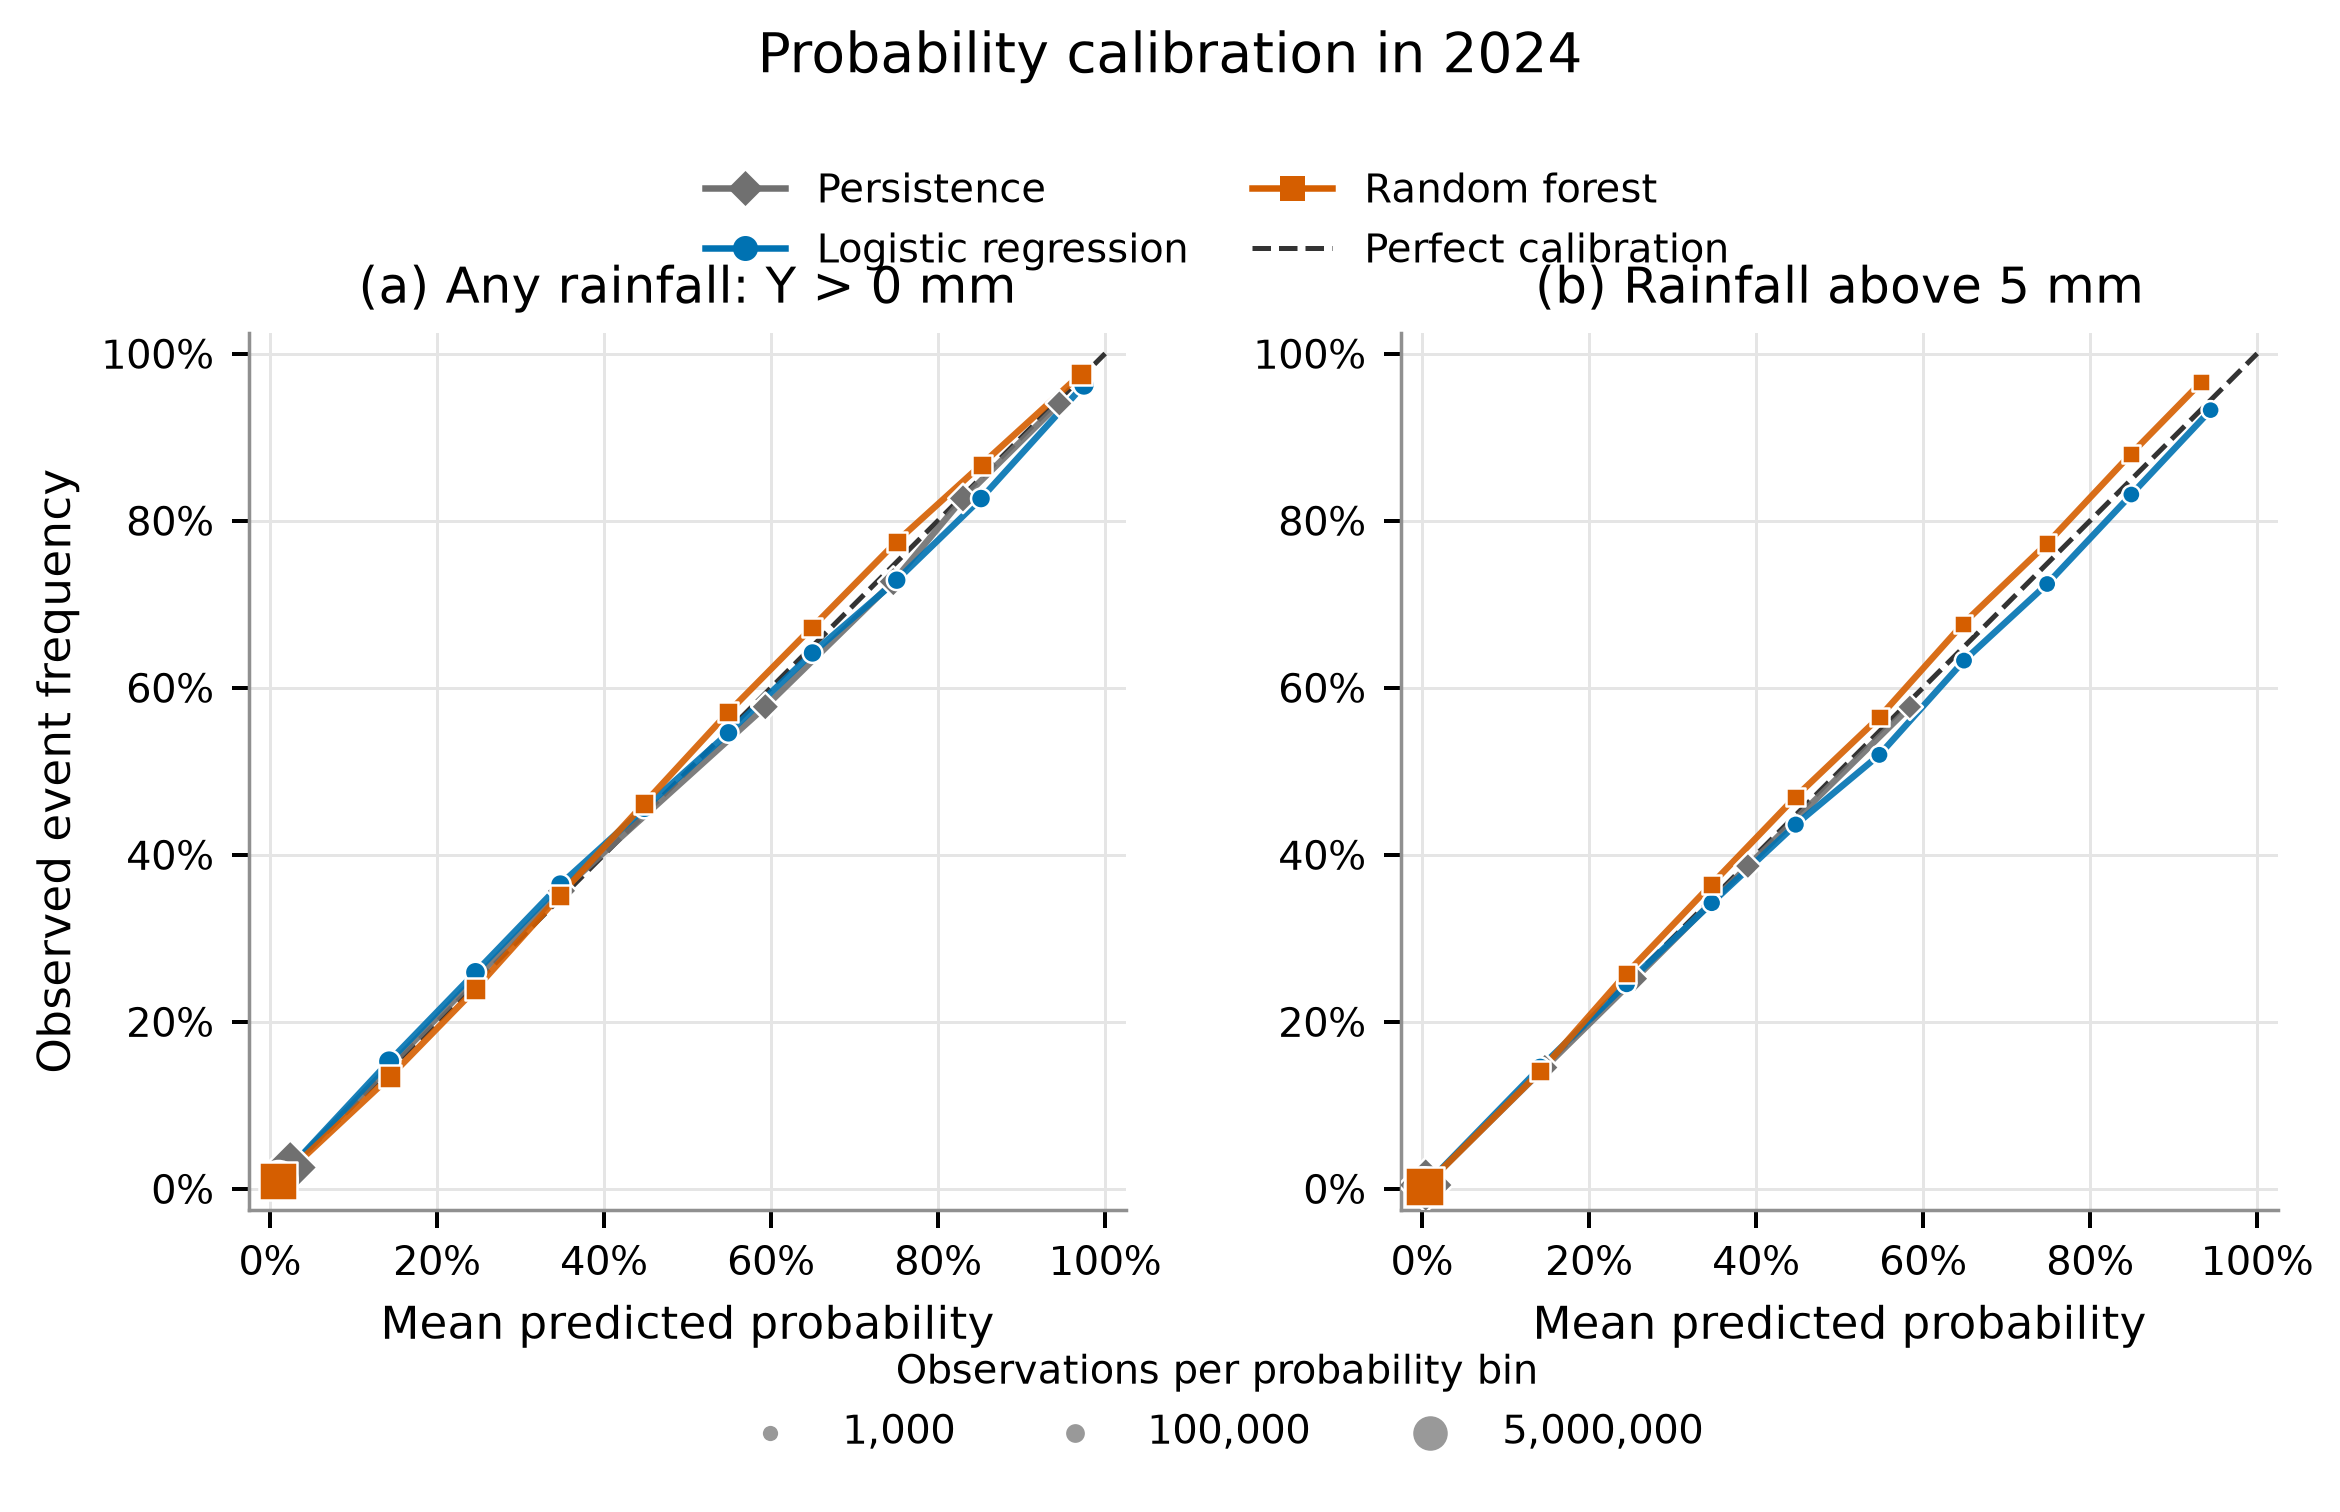
\includegraphics[width=0.94\linewidth,height=0.43\textheight,keepaspectratio]{figures/reliability_2024.png}
\caption{Probability calibration in 2024 for any rainfall and rainfall above \(5\,\mathrm{mm}\). Marker size indicates the number of observations in each probability bin. The dashed diagonal represents perfect calibration.}
\label{fig:reliability}
\end{figure}


Performance across rainfall thresholds was assessed using the Brier skill score relative to climatology~\citep{weigel2007}:


\[
\mathrm{BSS}=1-\frac{\text{Brier score}(\text{model})}{\text{Brier score}(\text{climatology})}.
\]


\begin{figure}[!htbp]
\centering
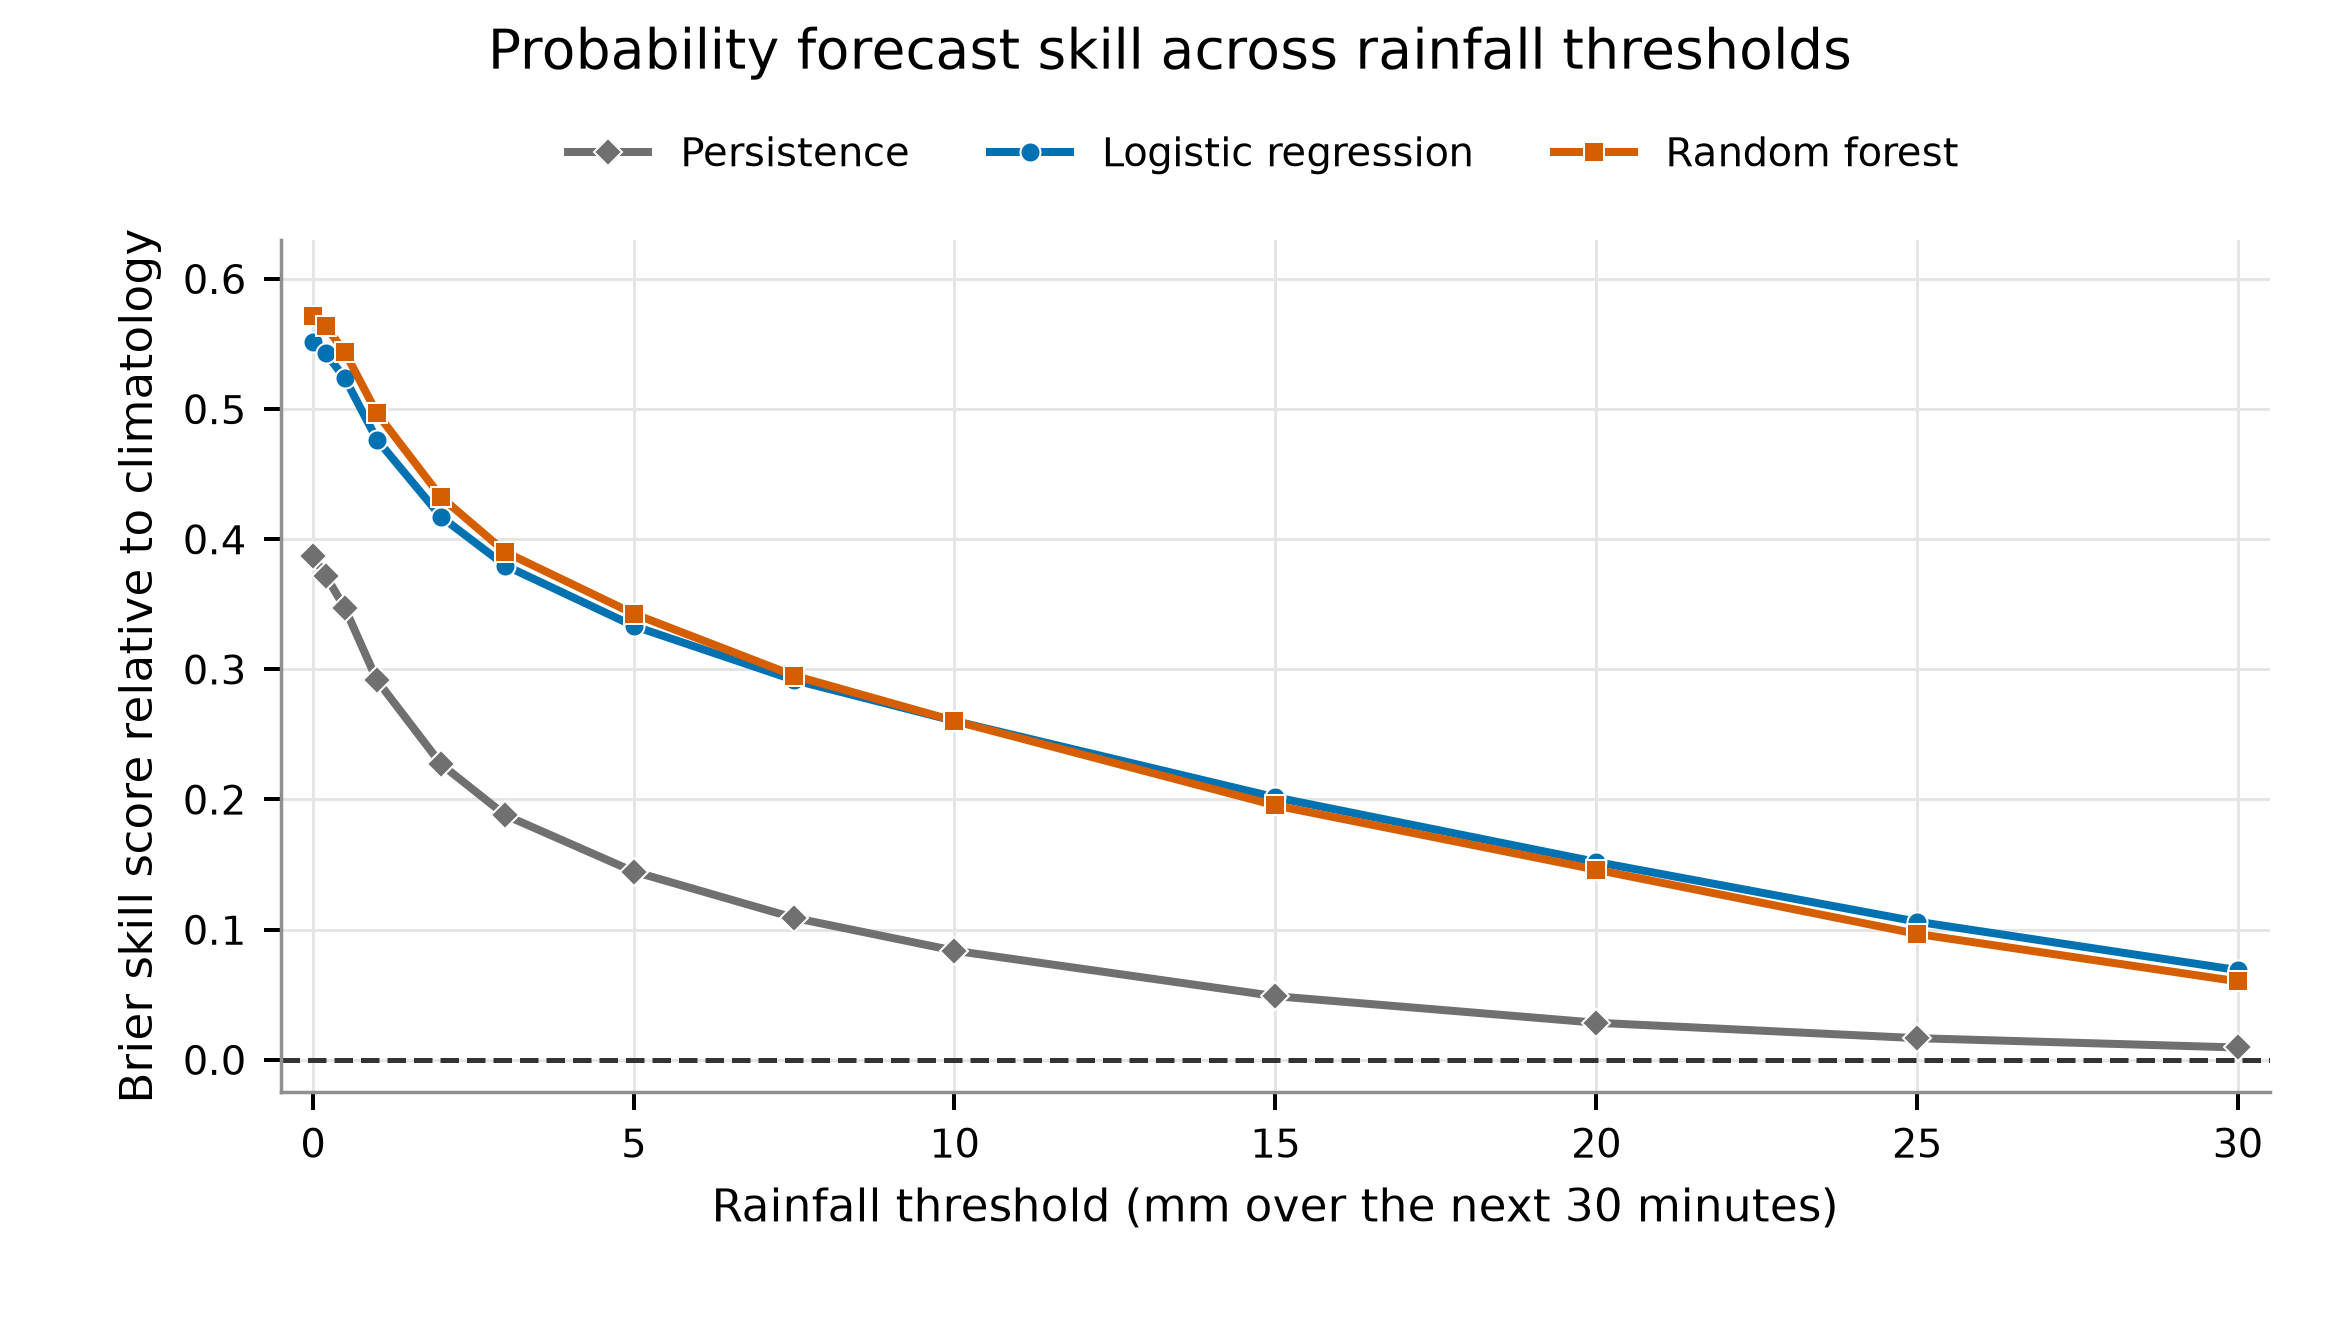
\includegraphics[width=0.91\linewidth,height=0.39\textheight,keepaspectratio]{figures/threshold_skill_2024.png}
\caption{Brier skill relative to climatology across rainfall thresholds in 2024. Positive values indicate lower Brier scores than climatology.}
\label{fig:threshold-skill}
\end{figure}


Positive values indicate improvement over climatology. Both LR and RF also outperformed persistence at every evaluated threshold. RF achieved BSS values of 0.571 for any rainfall and 0.343 for rainfall exceeding \(5\,\mathrm{mm}\). Its skill declined to 0.146 at \(20\,\mathrm{mm}\) and 0.060 at \(30\,\mathrm{mm}\), showing more limited improvement for extreme rainfall.


RF had slightly higher Brier skill than LR at thresholds up to \(10\,\mathrm{mm}\), while LR performed slightly better at the evaluated thresholds from 15 to \(30\,\mathrm{mm}\). At \(30\,\mathrm{mm}\), LR achieved a BSS of 0.069 compared with RF’s 0.060. Only \(0.0295\%\) of test samples exceeded this threshold, highlighting the rarity of these outcomes. RF’s stronger overall RPS therefore did not translate into better probability forecasts at every rainfall threshold.


\subsection*{6.4 Error Analysis and Case Study}
\phantomsection
\addcontentsline{toc}{subsection}{\numberline{6.4}Error Analysis and Case Study}


\subsubsection*{6.4.1 Prediction Performance under Different Conditions.}
\phantomsection
\addcontentsline{toc}{subsubsection}{\numberline{6.4.1}Prediction Performance under Different Conditions.}


Performance was examined across recent rainfall conditions, hours, and stations to identify situations in which prediction remained difficult.


\Needspace{4\baselineskip}
\begingroup
\small
\setlength{\parskip}{0pt}
\renewcommand{\arraystretch}{1.18}
\begin{longtable}{@{}>{\raggedright\arraybackslash}p{(\linewidth-6\tabcolsep)*\real{0.37}}>{\raggedright\arraybackslash}p{(\linewidth-6\tabcolsep)*\real{0.23}}>{\raggedright\arraybackslash}p{(\linewidth-6\tabcolsep)*\real{0.2}}>{\raggedright\arraybackslash}p{(\linewidth-6\tabcolsep)*\real{0.2}}@{}}
\caption*{\textbf{Table 6.4.} AUC-PR for predicting any rainfall under different recent rainfall conditions in 2024.}\\
\toprule
\textbf{Preceding 30 minutes} & \textbf{Event prevalence} & \textbf{LR AUC-PR} & \textbf{RF AUC-PR} \\
\midrule
\endfirsthead
\toprule
\textbf{Preceding 30 minutes} & \textbf{Event prevalence} & \textbf{LR AUC-PR} & \textbf{RF AUC-PR} \\
\midrule
\endhead
Dry & \(2.5\%\) & 0.396 & 0.430 \\
Wet & \(62.7\%\) & 0.932 & 0.943 \\
\bottomrule
\end{longtable}
\endgroup


\textit{Note: Dry and wet indicate zero and positive rainfall totals during the preceding 30 minutes, respectively, and differ from the daily wet-day classification used in Task 1. The predicted event is any rainfall during the following 30 minutes. Event prevalence provides a no-ranking reference for AUC-PR.}


RF\textbf{ }achieved higher AUC-PR than LR under both dry and wet conditions. Both models showed predictive skill under dry conditions, suggesting an ability to anticipate the start of rainfall. AUC-PR was higher under wet conditions, but rainfall events were also much more frequent in this group. However, the higher scores under wet conditions should be interpreted alongside their substantially higher event prevalence.


RF’s RPS varied from 0.022 at midnight to 0.200 at 15:00, coinciding with more frequent afternoon rainfall rather than necessarily indicating poorer relative skill. RF achieved the lowest RPS among the five methods at 69 of 70 stations. The exception was S102, where persistence slightly outperformed RF (0.0597 versus 0.0644). Its limited evaluation sample of 6,469 observations warrants cautious interpretation.


\subsubsection*{6.4.2 Extreme-rainfall case study}
\phantomsection
\addcontentsline{toc}{subsubsection}{\numberline{6.4.2}Extreme-rainfall case study}


We examined a heavy rainfall event at station S90 on 29 December 2024. The peak 30-minute rainfall total reached \(65\,\mathrm{mm}\), the highest observed in the 2024 evaluation dataset. At 15:15 Singapore time, the preceding 30 minutes were dry, but the following 30 minutes accumulated \(27\,\mathrm{mm}\). LR and RF assigned probabilities of \(43.0\%\) and \(38.7\%\) to any rainfall, compared with only \(2.4\%\) for persistence. However, their probabilities of exceeding \(5\,\mathrm{mm}\) remained relatively low at \(13.4\%\) and \(11.8\%\). This illustrates the difficulty of anticipating intense rainfall before it is observed locally.


The models also responded more effectively to rainfall decay. At 17:30, the preceding 30-minute total was \(30.6\,\mathrm{mm}\), but the following total was only \(0.8\,\mathrm{mm}\). Persistence still assigned a \(58.4\%\) probability of exceeding \(5\,\mathrm{mm}\), compared with \(3.1\%\) for LR and \(10.4\%\) for RF.


\begin{figure}[!htbp]
\centering
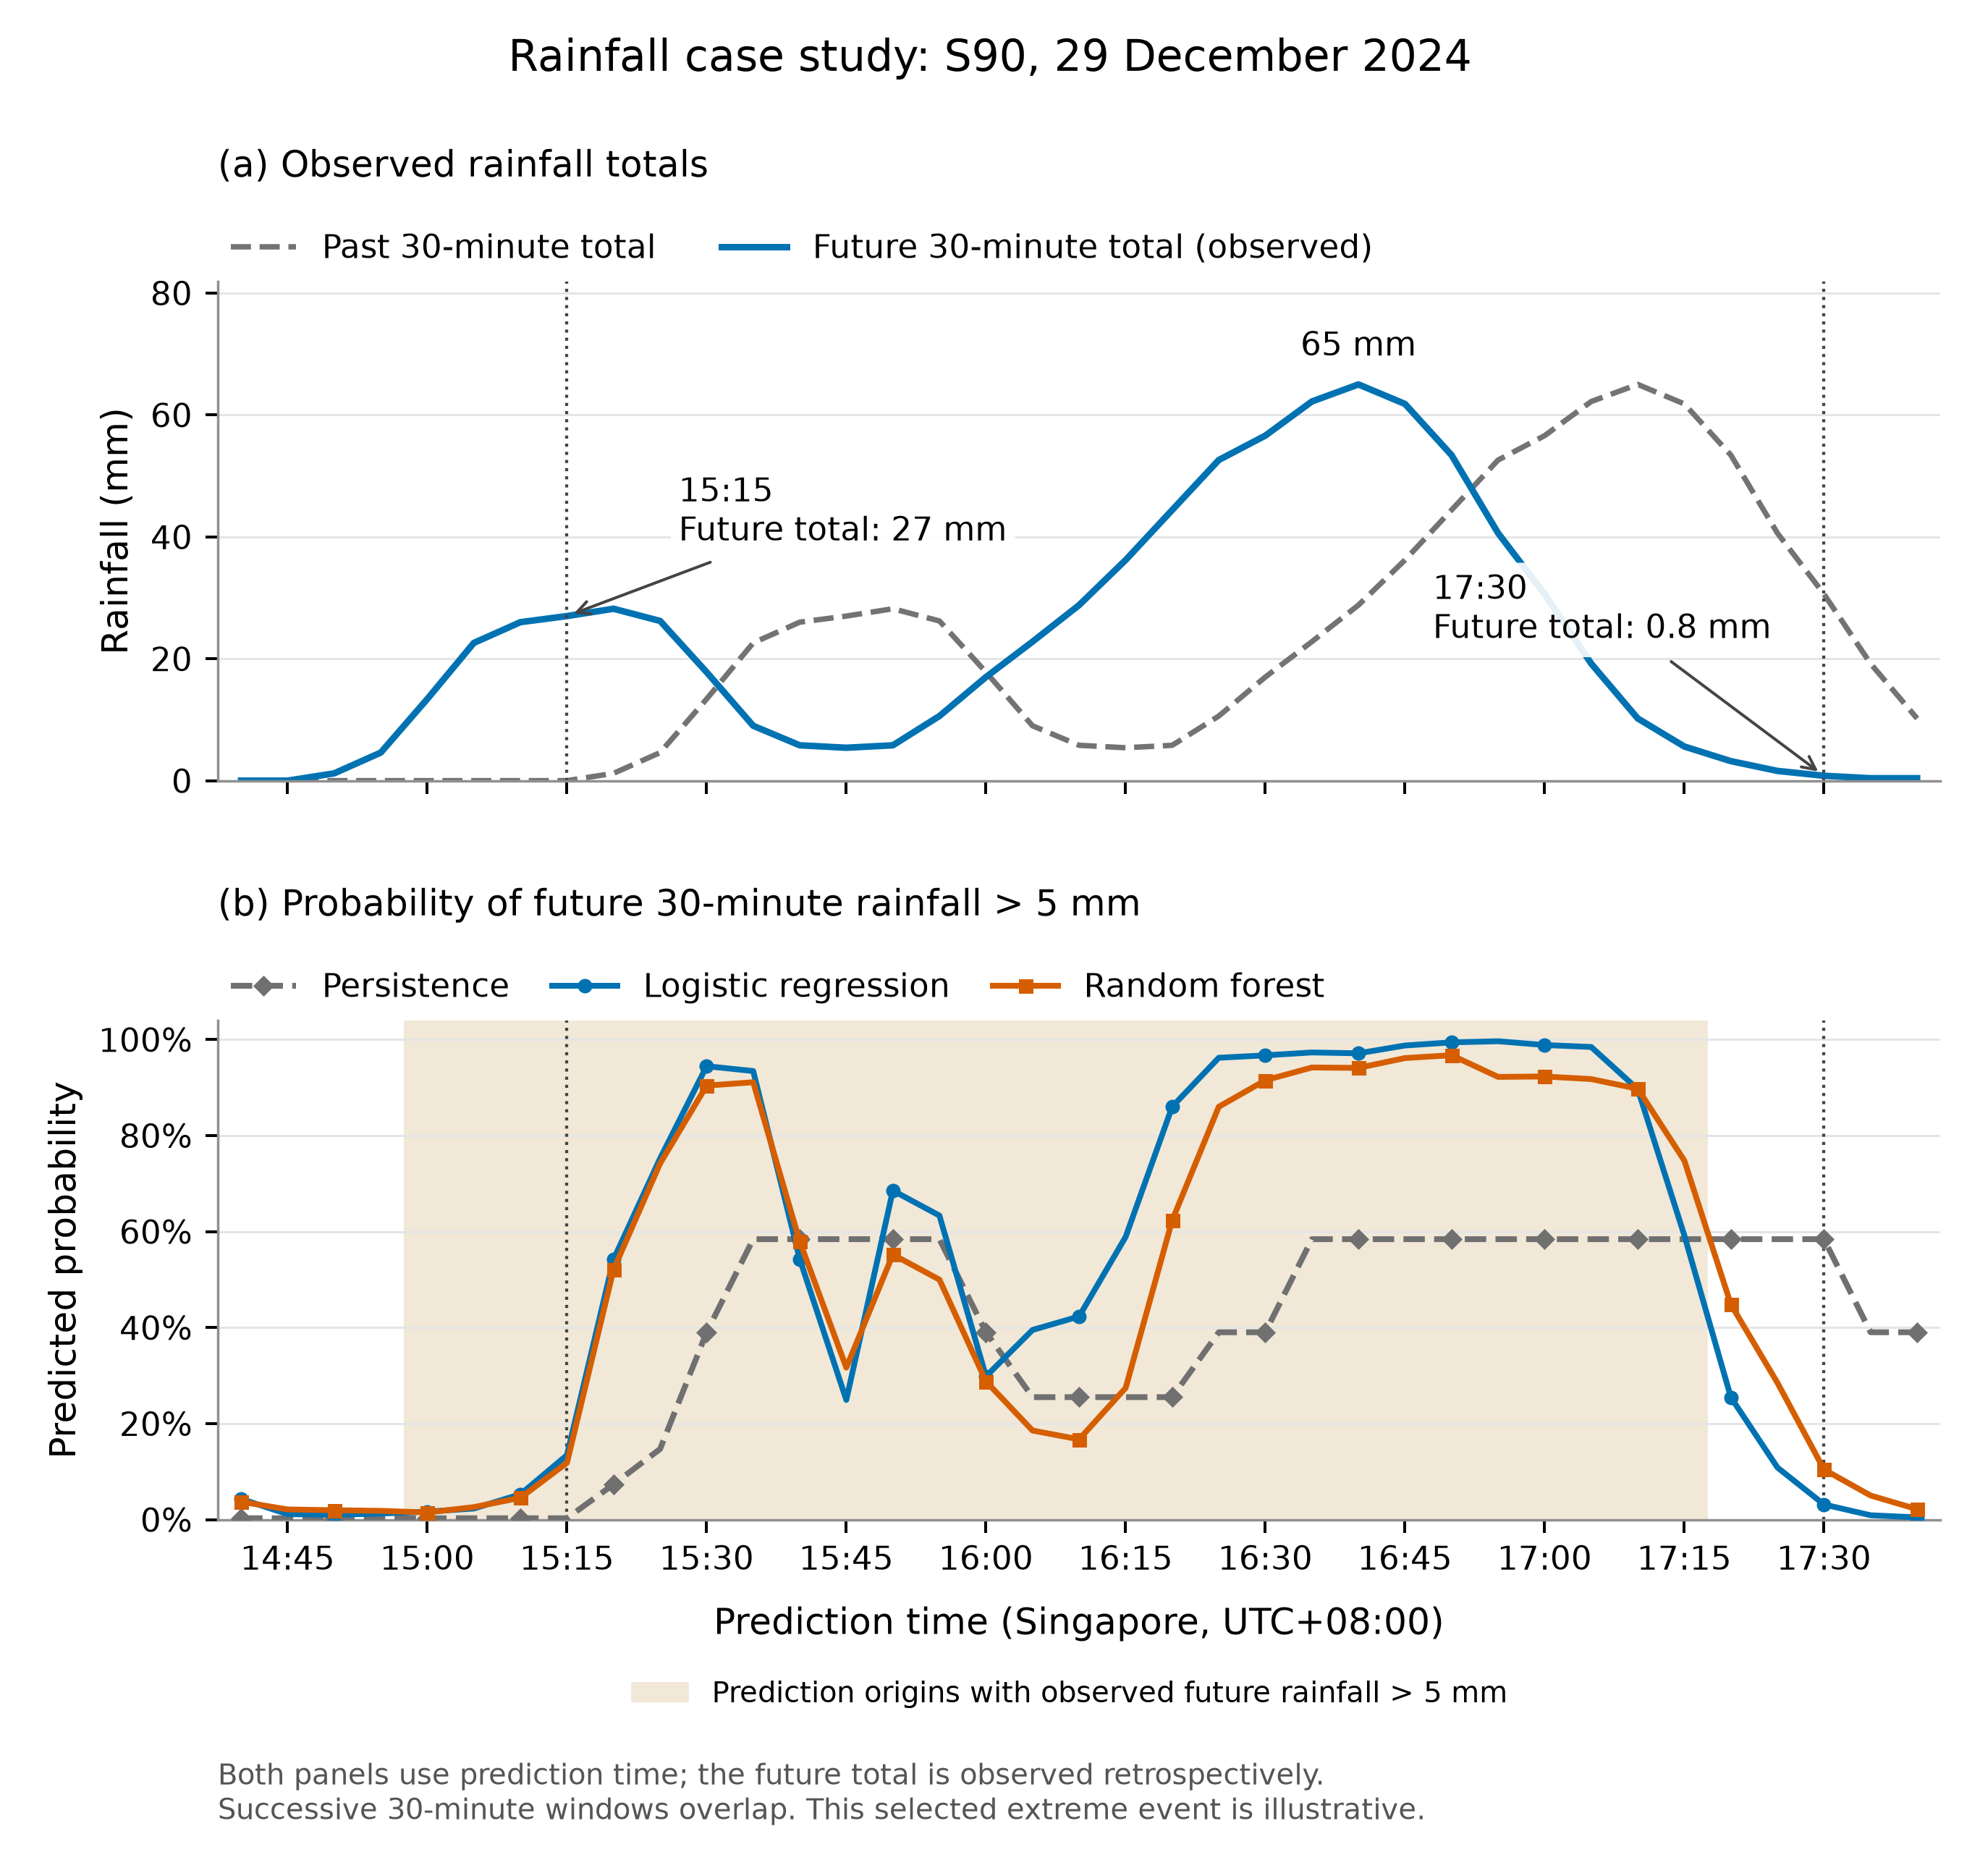
\includegraphics[width=0.94\linewidth,height=0.51\textheight,keepaspectratio]{figures/case_study_S90_20241229_gt5mm.png}
\caption{Rainfall and predicted exceedance probabilities at S90 on 29 December 2024. Both panels use prediction time in Singapore. Shading marks prediction origins whose observed future 30-minute rainfall exceeds \(5\,\mathrm{mm}\).}
\label{fig:case-study}
\end{figure}


Overall, the case illustrates improvements over persistence in anticipating rainfall onset and cessation, while highlighting limitations in anticipating sudden intensification. The event was selected retrospectively because of its extreme rainfall, and the prediction windows overlap. It therefore illustrates model behaviour in one event and should not be generalised to all storms.


\FloatBarrier

\section*{7. Limitations and Further Work}
\phantomsection
\addcontentsline{toc}{section}{\numberline{7.}Limitations and Further Work}


\subsection*{7.1 Data Quality and Station Coverage}
\phantomsection
\addcontentsline{toc}{subsection}{\numberline{7.1}Data Quality and Station Coverage}


Station coverage changed across years, and some records contained long gaps or suspected sensor faults. Coverage filters and exposure-normalised summaries reduce these problems but cannot eliminate selection bias. Missingness may depend on weather or equipment conditions, so retained observations may not represent all conditions. Statistical checks can also identify suspicious sensor behaviour without confirming its physical cause. Further work should test alternative quality-control rules, compare a consistent panel of stations, and seek maintenance records to validate sensor exclusions.


\subsection*{7.2 Retrospective versus Operational Prediction}
\phantomsection
\addcontentsline{toc}{subsection}{\numberline{7.2}Retrospective versus Operational Prediction}


The experiments use archived observations rather than a live reporting stream. Reporting delays and subsequent updates mean that a reading dated before the prediction time may not have been available then. Operational evaluation should reconstruct feature availability using reporting timestamps and exclude information received after each forecast origin.


The seasonal storm-motion prior was also estimated from 2017–2024 data, including the validation and test years. Consequently, the reported results are retrospective and do not establish fully independent out-of-sample performance. A stricter evaluation should re-estimate all data-derived priors and preprocessing decisions within each training period. The effect of this information reuse has not been quantified.


\subsection*{7.3 Temporal Scope and Dependence}
\phantomsection
\addcontentsline{toc}{subsection}{\numberline{7.3}Temporal Scope and Dependence}


Eight years are insufficient to establish long-term climate trends, and a single evaluation year provides limited evidence of performance under changing conditions. Overlapping 30-minute targets and shared storms also make observations dependent across times and stations. Rolling-origin evaluation across several years, with uncertainty estimates that preserve temporal and spatial dependence, would provide stronger evidence of generalisation.


\subsection*{7.4 Model Representation and Missing Information}
\phantomsection
\addcontentsline{toc}{subsection}{\numberline{7.4}Model Representation and Missing Information}


Rainfall is represented by nine classes. Probabilities at thresholds within a class depend on the training-derived within-bin distribution, which does not vary with the prediction context. Rare extremes provide limited training evidence, and the empirical threshold mapper cannot extrapolate beyond observed training amounts. Continuous or hybrid distributional models could address these limitations.


The models use rainfall, station, and calendar information but lack direct measurements of wind, humidity, temperature, and radar reflectivity. Calendar-based monsoon indicators cannot represent the atmospheric conditions of individual storms. These limitations constrain rainfall-onset prediction and prevent causal attribution of observed patterns to particular meteorological mechanisms.


\subsection*{7.5 Computational Constraints and Extensions}
\phantomsection
\addcontentsline{toc}{subsection}{\numberline{7.5}Computational Constraints and Extensions}


Model comparison was restricted to LR, RF, and three baselines. The implementation supports weighted dry-period subsampling to reduce development costs, but sensitivity to alternative sampling designs requires further evaluation. Useful extensions include broader tuning, an onset-specific model, and additional meteorological inputs. Larger computing resources would support repeated refitting and rolling-origin comparisons, but performance gains would still require empirical validation.


\FloatBarrier

\section*{8. Conclusion}
\phantomsection
\addcontentsline{toc}{section}{\numberline{8.}Conclusion}


This project used Apache Spark to investigate Singapore’s five-minute rainfall observations from 2017 to 2024 and develop probabilistic forecasts for the following 30 minutes.


For Task 1, the analysis identified seasonal and diurnal variation, spatial differences between stations, and persistence across consecutive days. The afternoon rainfall peak was driven more by rainfall frequency than by intensity. Nearby stations showed correlated rainfall, with correlation extending over larger distances at longer aggregation intervals. The analysis also identified 2019 as the driest year within the study period, without establishing a long-term trend or its meteorological cause.


For Task 2, both LR and RF improved on the constant, climatology, and persistence baselines in the 2024 retrospective evaluation. RF achieved the lowest overall RPS of 0.0887, compared with 0.0922 for LR and 0.1246 for persistence. Feature-permutation results showed substantial reliance on recent local and neighbouring rainfall. However, sudden rainfall onset and rare extremes remained challenging. Incomplete observations, reporting delays, and the use of a full-period storm-motion prior limit operational and out-of-sample interpretation. The results support the predictive value of rainfall history and spatial context, while motivating a stricter leakage-free evaluation before deployment.


\clearpage

\section*{9. Declaration of AI Usage}
\phantomsection
\addcontentsline{toc}{section}{\numberline{9.}Declaration of AI Usage}


We acknowledge the use of ChatGPT/Codex (OpenAI) in preparing this project. AI tools supported code development, analysis planning, visualisation, documentation and report preparation, as described below.

\subsection*{Claude}

Claude (Anthropic) generated most of the project code, including:
\begin{itemize}
    \item the data-quality audit and preprocessing scripts, including timestamp alignment, duplicate resolution, and conversion to Parquet;
    \item the Task 1 rainfall aggregation, station-matrix construction, and visualisation scripts;
    \item the Task 2 label construction, feature engineering, logistic regression and random forest training, hyperparameter tuning, and evaluation pipelines;
    \item the prediction, result-plotting, and rainfall-replay scripts.
\end{itemize}

\subsection*{ChatGPT/Codex}
ChatGPT/Codex was used as a supporting tool for proofreading grammatical errors in the
report, improving formatting and presentation, reviewing the project code for consistency with
the assignment requirements, and refining the clarity, organisation, and expression of the written
report.

\subsection*{Review and verification}

AI-assisted code execution and inspection were used to check preprocessing row counts, selected exported evaluation values and generated figures. These checks are limited to the files and outputs inspected and do not constitute an independent audit or establish that every reported result has been verified.

\subsection*{Responsibility for the submission}

AI assistance does not replace the observed rainfall data, experiment outputs, software documentation or the authors' scientific judgement. The group is responsible for reviewing AI-assisted code, interpretations, references and written material, and for the content, accuracy, originality and quality of the submission. Reported findings must be supported by the project data and results rather than AI-generated assertions.


\clearpage

\bibliographystyle{unsrtnat}
\bibliography{references}


\clearpage

\section*{Appendices}
\phantomsection
\addcontentsline{toc}{section}{Appendices}

\subsection*{Appendix A. Detailed Data-Quality Results}
\phantomsection
\addcontentsline{toc}{subsection}{Appendix A. Detailed Data-Quality Results}

The eight annual files hold 48,538,713 observations from 91 station IDs. Every record is a five-minute rainfall total in mm. No missing timestamp, station, rainfall, coordinate or update-time value, no negative or non-finite rainfall, and no duplicate original (station, timestamp) key was found in any year.

\begingroup
\small
\setlength{\parskip}{0pt}
\setlength{\tabcolsep}{3pt}
\renewcommand{\arraystretch}{1.16}
\begin{longtable}{@{}>{\raggedright\arraybackslash}p{(\linewidth-8\tabcolsep)*\real{0.09}}>{\raggedright\arraybackslash}p{(\linewidth-8\tabcolsep)*\real{0.14}}>{\raggedright\arraybackslash}p{(\linewidth-8\tabcolsep)*\real{0.12}}>{\raggedright\arraybackslash}p{(\linewidth-8\tabcolsep)*\real{0.325}}>{\raggedright\arraybackslash}p{(\linewidth-8\tabcolsep)*\real{0.325}}@{}}
\caption*{\textbf{Table A.1.} Dataset overview by year}\\
\toprule
\textbf{Year} & \textbf{Rows} & \textbf{Stations} & \textbf{First observation} & \textbf{Last observation} \\
\midrule
\endfirsthead
\toprule
\textbf{Year} & \textbf{Rows} & \textbf{Stations} & \textbf{First observation} & \textbf{Last observation} \\
\midrule
\endhead
2017 & 5,256,106 & 62 & 2017-01-01 08:04:59 & 2017-12-31 23:55:00 \\
2018 & 4,594,246 & 56 & 2018-01-01 00:00:00 & 2018-12-31 23:55:00 \\
2019 & 5,026,862 & 54 & 2019-01-01 00:00:00 & 2019-12-31 23:55:00 \\
2020 & 6,334,473 & 80 & 2020-01-01 00:00:00 & 2020-12-31 23:55:00 \\
2021 & 7,044,646 & 76 & 2021-01-01 00:00:00 & 2021-12-31 23:55:00 \\
2022 & 7,133,230 & 72 & 2022-01-01 00:00:00 & 2022-12-31 23:55:00 \\
2023 & 6,742,890 & 74 & 2023-01-01 00:00:00 & 2023-12-31 23:55:00 \\
2024 & 6,406,260 & 70 & 2024-01-01 00:00:00 & 2024-12-31 23:55:00 \\
\textbf{Total} & \textbf{48,538,713} & \textbf{91 unique} &  &  \\
\bottomrule
\end{longtable}
\endgroup

Coverage is the share of the expected five-minute records that a station reported between its own first and last observation in that year, so a station that joined or left during the year is not penalised. It differs from the calendar-based coverage of Section 3.3 and Figure 1, which counts against the full month or year. The audit coverage is diagnostic: it was not used to delete any station.

\begingroup
\small
\setlength{\parskip}{0pt}
\setlength{\tabcolsep}{3pt}
\renewcommand{\arraystretch}{1.16}
\begin{longtable}{@{}>{\raggedright\arraybackslash}p{(\linewidth-10\tabcolsep)*\real{0.08}}>{\raggedright\arraybackslash}p{(\linewidth-10\tabcolsep)*\real{0.12}}>{\raggedright\arraybackslash}p{(\linewidth-10\tabcolsep)*\real{0.17}}>{\raggedright\arraybackslash}p{(\linewidth-10\tabcolsep)*\real{0.17}}>{\raggedright\arraybackslash}p{(\linewidth-10\tabcolsep)*\real{0.23}}>{\raggedright\arraybackslash}p{(\linewidth-10\tabcolsep)*\real{0.23}}@{}}
\caption*{\textbf{Table A.2.} Station coverage by year}\\
\toprule
\textbf{Year} & \textbf{Stations} & \textbf{Mean coverage} & \textbf{Median coverage} & \textbf{Stations below 80\%} & \textbf{Stations below 50\%} \\
\midrule
\endfirsthead
\toprule
\textbf{Year} & \textbf{Stations} & \textbf{Mean coverage} & \textbf{Median coverage} & \textbf{Stations below 80\%} & \textbf{Stations below 50\%} \\
\midrule
\endhead
2017 & 62 & 0.8972 & 0.9497 & 5 & 3 \\
2018 & 56 & 0.8110 & 0.8179 & 17 & 0 \\
2019 & 54 & 0.9030 & 0.9490 & 8 & 2 \\
2020 & 80 & 0.9144 & 0.9481 & 5 & 2 \\
2021 & 76 & 0.9563 & 0.9842 & 3 & 1 \\
2022 & 72 & 0.9775 & 0.9975 & 2 & 1 \\
2023 & 74 & 0.9331 & 0.9677 & 2 & 2 \\
2024 & 70 & 0.9608 & 0.9835 & 2 & 0 \\
\bottomrule
\end{longtable}
\endgroup

Source: \path{task1/results/data_quality_audit/yearly_quality.csv} and \path{coverage_by_year.csv}, written by \path{task1/code/rainfall_audit.py}; discussion in \path{task1/docs/data_quality_findings.md}.

\clearpage
\subsection*{Appendix B. Full Feature Definitions}
\phantomsection
\addcontentsline{toc}{subsection}{Appendix B. Full Feature Definitions}

\begingroup
\small
\setlength{\parskip}{0pt}
\setlength{\tabcolsep}{3pt}
\renewcommand{\arraystretch}{1.16}
\begin{longtable}{@{}>{\raggedright\arraybackslash}p{(\linewidth-8\tabcolsep)*\real{0.055}}>{\raggedright\arraybackslash}p{(\linewidth-8\tabcolsep)*\real{0.255}}>{\raggedright\arraybackslash}p{(\linewidth-8\tabcolsep)*\real{0.05}}>{\raggedright\arraybackslash}p{(\linewidth-8\tabcolsep)*\real{0.43}}>{\raggedright\arraybackslash}p{(\linewidth-8\tabcolsep)*\real{0.21}}@{}}
\caption*{\textbf{Table B.1.} Features}\\
\toprule
\textbf{Tier} & \textbf{Feature(s)} & \textbf{No.} & \textbf{How it is constructed} & \textbf{Data used} \\
\midrule
\endfirsthead
\toprule
\textbf{Tier} & \textbf{Feature(s)} & \textbf{No.} & \textbf{How it is constructed} & \textbf{Data used} \\
\midrule
\endhead
T0 & \path{t0_x_km}, \path{t0_y_km} & 2 & Station position in km east and north of the island centre (103.82\(^{\circ}\)E, 1.35\(^{\circ}\)N), by an equirectangular projection & Latest station coordinates \\
T0 & \path{t0_wet_ratio} & 1 & (O + 500) / (E + 500): rainy 30-minute windows observed at the station (Y \(>\) 0), over the number expected if it followed the network at the same times; shrunk towards 1 & Labels 2017--2022, constant per station \\
T0 & \path{t0_heavy_ratio} & 1 & The same ratio for heavy windows (Y \(>\) 5 mm) & Labels 2017--2022, constant per station \\
T0 & \path{t0_hod_s1}--\path{s3}, \path{t0_hod_c1}--\path{c3} & 6 & sin and cos of 2\(\pi\)k\(\cdot\)h/24 for k = 1, 2, 3, where h is the local hour of the prediction time (with minutes) & Prediction time \\
T0 & \path{t0_doy_s1}, \path{s2}, \path{t0_doy_c1}, \path{c2} & 4 & sin and cos of 2\(\pi\)k\(\cdot\)\(\delta\) for k = 1, 2, where \(\delta\) is the fraction of the year elapsed & Prediction time \\
T0 & \path{t0_season} & 1 & Monsoon code: 0 for Dec--Mar, 2 for Jun--Sep, 1 otherwise & Prediction time \\
T1 & \path{t1_rain_5}, \path{t1_rain_15}, \path{t1_rain_30}, \path{t1_rain_60}, \path{t1_rain_120}, \path{t1_rain_1440} & 6 & Rain total at the station over the last 5, 15, 30, 60, 120 and 1,440 minutes (\path{t1_rain_5} is the current reading) & Station's own readings, t and earlier \\
T1 & \path{t1_max5_30} & 1 & Largest five-minute reading in the last 30 minutes & Same \\
T1 & \path{t1_wet_slots_60} & 1 & Number of wet readings among the last 12 & Same \\
T1 & \path{t1_trend_30} & 1 & 2\(\cdot\)\(R^{15}\) \(-\) \(R^{30}\): the last 15 minutes minus the 15 minutes before, positive when rain is intensifying & Same \\
T1 & \path{t1_min_since_rain} & 1 & Minutes since the last wet reading, capped at 1,440 & Same \\
T1 & \path{t1_missing_120} & 1 & Number of missing readings among the last 24 & Same \\
T2 & \path{t2_idw_rain_15}, \path{t2_idw_rain_30} & 2 & Mean 15- and 30-minute rain of the other stations within 10 km, weighted by \(1/\max(d,0.5)^2\), reporting stations only (0 if none) & Other stations, time t \\
T2 & \path{t2_idw_trend} & 1 & 2 \(\times\) \path{t2_idw_rain_15} \(-\) \path{t2_idw_rain_30}, the neighbours' version of the trend & Same \\
T2 & \path{t2_far_rain_30} & 1 & The same weighted mean of 30-minute rain for stations 10 to 25 km away & Same \\
T2 & \path{t2_max_rain_30} & 1 & Largest 30-minute rain at any reporting station within 10 km & Same \\
T2 & \path{t2_wet_frac_5km}, \path{t2_wet_frac_10km} & 2 & Share of reporting stations within 5 km and 10 km with rain in the last 30 minutes & Same \\
T2 & \path{t2_dist_rain_km} & 1 & Distance to the nearest station with rain in the last 15 minutes, capped at 30 km & Same \\
T2 & \path{t2_rain_30_n}, \path{_e}, \path{_s}, \path{_w} & 4 & Mean 30-minute rain of the reporting stations within 25 km in the north, east, south and west quadrants & Same \\
T2 & \path{t2_island_wet_frac}, \path{t2_island_rain_30} & 2 & Share of all reporting stations that are wet, and their mean 30-minute rain & All stations, time t \\
T2 & \path{t2_nbrs_10km} & 1 & Number of reporting stations within 10 km (tells the model how many stations the averages rest on) & Other stations, time t \\
T3 & \path{t3_d15_idw_rain_30}, \path{_far_rain_30}, \path{_max_rain_30}, \path{_wet_frac_5km}, \path{_wet_frac_10km}, \path{_dist_rain_km}, \path{_rain_30_n}, \path{_e}, \path{_s}, \path{_w}, \path{_island_wet_frac}, \path{_island_rain_30} & 12 & Each of these twelve Tier 2 summaries now, minus the same summary recomputed from the network readings 15 minutes earlier & Network at t and at t \(-\) 15 min \\
T3 & \path{t3_up15_rain}, \path{t3_up15_wet} & 2 & Gaussian-weighted mean (\(\sigma\) = 4 km, cut-off 10 km) of 15-minute rain, and of the wet indicator, around the point 15 minutes upstream: the station moved backwards along the seasonal storm motion (Table 5.3) & Network at t \\
T3 & \path{t3_up30_rain}, \path{t3_up30_wet} & 2 & The same around the point 30 minutes upstream & Network at t \\
T3 & \path{t3_up30_nbrs} & 1 & Number of stations near the 30-minute upstream point (it separates "dry" from "no gauge there") & Network at t \\
\bottomrule
\end{longtable}
\endgroup

\clearpage
\subsection*{Appendix C. Hyperparameter Tuning and Test Performance}
\phantomsection
\addcontentsline{toc}{subsection}{Appendix C. Hyperparameter Tuning and Test Performance}

\begingroup
\small
\setlength{\parskip}{0pt}
\setlength{\tabcolsep}{3pt}
\renewcommand{\arraystretch}{1.16}
\begin{longtable}{@{}>{\raggedright\arraybackslash}p{(\linewidth-10\tabcolsep)*\real{0.2}}>{\raggedright\arraybackslash}p{(\linewidth-10\tabcolsep)*\real{0.15}}>{\raggedright\arraybackslash}p{(\linewidth-10\tabcolsep)*\real{0.18}}>{\raggedright\arraybackslash}p{(\linewidth-10\tabcolsep)*\real{0.17}}>{\raggedright\arraybackslash}p{(\linewidth-10\tabcolsep)*\real{0.13}}>{\raggedright\arraybackslash}p{(\linewidth-10\tabcolsep)*\real{0.17}}@{}}
\caption*{\textbf{Table C.1.} Logistic regression on the 2023 validation set}\\
\toprule
\textbf{Tiers} & \textbf{\(\lambda\) (regParam)} & \textbf{Non-linear inputs} & \textbf{Validation RPS} & \textbf{Iterations} & \textbf{Fit (min)} \\
\midrule
\endfirsthead
\toprule
\textbf{Tiers} & \textbf{\(\lambda\) (regParam)} & \textbf{Non-linear inputs} & \textbf{Validation RPS} & \textbf{Iterations} & \textbf{Fit (min)} \\
\midrule
\endhead
T0+T1+T2 & 1e-05 & no & 0.0961 & 429 & 4.7 \\
T0+T1+T2 & 1e-06 & yes & 0.0935 & 659 & 10.7 \\
T0+T1+T2 & 1e-05 & yes & 0.0936 & 609 & 9.9 \\
T0+T1+T2 & 0.0001 & yes & 0.0937 & 530 & 8.8 \\
T0+T1+T2+T3 & 1e-06 & yes & 0.0922 & 655 & 12.9 \\
\bottomrule
\end{longtable}
\endgroup

The first row is the plain model; the last row adds Tier 3 and is the final specification.

Rows are in the order tried; the last row is the chosen setting before Tier 3 was added.

\begingroup
\footnotesize
\setlength{\parskip}{0pt}
\setlength{\tabcolsep}{3pt}
\renewcommand{\arraystretch}{1.16}
\begin{longtable}{@{}>{\raggedright\arraybackslash}p{(\linewidth-14\tabcolsep)*\real{0.1}}>{\raggedright\arraybackslash}p{(\linewidth-14\tabcolsep)*\real{0.14}}>{\raggedright\arraybackslash}p{(\linewidth-14\tabcolsep)*\real{0.2}}>{\raggedright\arraybackslash}p{(\linewidth-14\tabcolsep)*\real{0.1}}>{\raggedright\arraybackslash}p{(\linewidth-14\tabcolsep)*\real{0.1}}>{\raggedright\arraybackslash}p{(\linewidth-14\tabcolsep)*\real{0.13}}>{\raggedright\arraybackslash}p{(\linewidth-14\tabcolsep)*\real{0.11}}>{\raggedright\arraybackslash}p{(\linewidth-14\tabcolsep)*\real{0.12}}@{}}
\caption*{\textbf{Table C.2.} Random forest screening on 2023}\\
\toprule
\textbf{max\newline Depth} & \textbf{min\newline Instances\newline PerNode} & \textbf{featureSubset\newline Strategy} & \textbf{maxBins} & \textbf{Impurity} & \textbf{Validation RPS} & \textbf{Fit (min)} & \textbf{Nodes} \\
\midrule
\endfirsthead
\toprule
\textbf{max\newline Depth} & \textbf{min\newline Instances\newline PerNode} & \textbf{featureSubset\newline Strategy} & \textbf{maxBins} & \textbf{Impurity} & \textbf{Validation RPS} & \textbf{Fit (min)} & \textbf{Nodes} \\
\midrule
\endhead
14 & 100 & sqrt & 64 & gini & 0.0927 & 2.7 & 224,268 \\
17 & 100 & sqrt & 64 & gini & 0.0923 & 4.5 & 379,530 \\
20 & 100 & sqrt & 64 & gini & 0.0923 & 6.0 & 435,878 \\
24 & 100 & sqrt & 64 & gini & 0.0923 & 7.3 & 444,966 \\
24 & 20 & sqrt & 64 & gini & 0.0930 & 21.5 & 2,675,066 \\
24 & 50 & sqrt & 64 & gini & 0.0920 & 11.4 & 984,782 \\
24 & 300 & sqrt & 64 & gini & 0.0935 & 4.0 & 122,922 \\
24 & 50 & onethird & 64 & gini & 0.0919 & 20.3 & 1,014,978 \\
24 & 50 & 0.5 & 64 & gini & 0.0919 & 27.8 & 1,029,336 \\
24 & 50 & onethird & 256 & gini & 0.0912 & 56.1 & 1,030,260 \\
24 & 50 & onethird & 256 & entropy & 0.0911 & 63.8 & 1,044,176 \\
\bottomrule
\end{longtable}
\endgroup

RPS: ranked probability score; Brier \(>\)\(\theta\): Brier score of P(Y \(>\) \(\theta\)) in mm; AUC-PR: area under the precision-recall curve. Lower is better for RPS, log loss and Brier; higher for AUC-PR.

\begin{landscape}
\begingroup
\footnotesize
\setlength{\parskip}{0pt}
\setlength{\tabcolsep}{3pt}
\renewcommand{\arraystretch}{1.16}
\begin{longtable}{@{}>{\raggedright\arraybackslash}p{(\linewidth-22\tabcolsep)*\real{0.115}}>{\raggedright\arraybackslash}p{(\linewidth-22\tabcolsep)*\real{0.15}}>{\raggedright\arraybackslash}p{(\linewidth-22\tabcolsep)*\real{0.0735}}>{\raggedright\arraybackslash}p{(\linewidth-22\tabcolsep)*\real{0.0735}}>{\raggedright\arraybackslash}p{(\linewidth-22\tabcolsep)*\real{0.0735}}>{\raggedright\arraybackslash}p{(\linewidth-22\tabcolsep)*\real{0.0735}}>{\raggedright\arraybackslash}p{(\linewidth-22\tabcolsep)*\real{0.0735}}>{\raggedright\arraybackslash}p{(\linewidth-22\tabcolsep)*\real{0.0735}}>{\raggedright\arraybackslash}p{(\linewidth-22\tabcolsep)*\real{0.0735}}>{\raggedright\arraybackslash}p{(\linewidth-22\tabcolsep)*\real{0.0735}}>{\raggedright\arraybackslash}p{(\linewidth-22\tabcolsep)*\real{0.0735}}>{\raggedright\arraybackslash}p{(\linewidth-22\tabcolsep)*\real{0.0735}}@{}}
\caption*{\textbf{Table C.3.} Test year 2024}\\
\toprule
\textbf{Subset} & \textbf{Forecast} & \textbf{RPS} & \textbf{log loss} & \textbf{Brier \(>\)0} & \textbf{Brier \(>\)1} & \textbf{Brier \(>\)5} & \textbf{Brier \(>\)20} & \textbf{AUC-PR \(>\)0} & \textbf{AUC-PR \(>\)1} & \textbf{AUC-PR \(>\)5} & \textbf{AUC-PR \(>\)20} \\
\midrule
\endfirsthead
\toprule
\textbf{Subset} & \textbf{Forecast} & \textbf{RPS} & \textbf{log loss} & \textbf{Brier \(>\)0} & \textbf{Brier \(>\)1} & \textbf{Brier \(>\)5} & \textbf{Brier \(>\)20} & \textbf{AUC-PR \(>\)0} & \textbf{AUC-PR \(>\)1} & \textbf{AUC-PR \(>\)5} & \textbf{AUC-PR \(>\)20} \\
\midrule
\endhead
All forecasts & Constant & 0.1903 & 0.3545 & 0.0596 & 0.0244 & 0.00825 & 0.00103 & 0.0636 & 0.0250 & 0.0083 & 0.0010 \\
All forecasts & Climatology & 0.1864 & 0.3437 & 0.0578 & 0.0240 & 0.00820 & 0.00102 & 0.1254 & 0.0540 & 0.0234 & 0.0043 \\
All forecasts & Persistence & 0.1246 & 0.2577 & 0.0355 & 0.0170 & 0.00701 & 0.00100 & 0.6406 & 0.4731 & 0.2500 & 0.0495 \\
All forecasts & Logistic regression & 0.0922 & 0.1933 & 0.0259 & 0.0126 & 0.00547 & 0.00087 & 0.7850 & 0.6888 & 0.5066 & 0.1956 \\
All forecasts & Random forest & 0.0887 & 0.1863 & 0.0248 & 0.0121 & 0.00539 & 0.00088 & 0.8015 & 0.7117 & 0.5246 & 0.2285 \\
Dry now & Constant & 0.0708 & 0.1760 & 0.0260 & 0.0081 & 0.00275 & 0.00026 & 0.0253 & 0.0079 & 0.0027 & 0.0003 \\
Dry now & Climatology & 0.0710 & 0.1705 & 0.0259 & 0.0082 & 0.00277 & 0.00026 & 0.0522 & 0.0208 & 0.0084 & 0.0009 \\
Dry now & Persistence & 0.0679 & 0.1611 & 0.0247 & 0.0079 & 0.00272 & 0.00026 & 0.0253 & 0.0079 & 0.0027 & 0.0003 \\
Dry now & Logistic regression & 0.0544 & 0.1142 & 0.0187 & 0.0066 & 0.00243 & 0.00025 & 0.3962 & 0.2608 & 0.1616 & 0.0410 \\
Dry now & Random forest & 0.0530 & 0.1111 & 0.0182 & 0.0065 & 0.00241 & 0.00025 & 0.4298 & 0.2959 & 0.1903 & 0.0553 \\
Raining now & Constant & 1.9499 & 2.9833 & 0.5544 & 0.2635 & 0.08926 & 0.01232 & 0.6275 & 0.2759 & 0.0907 & 0.0123 \\
Raining now & Climatology & 1.8859 & 2.8948 & 0.5278 & 0.2578 & 0.08825 & 0.01228 & 0.6403 & 0.2977 & 0.1204 & 0.0236 \\
Raining now & Persistence & 0.9580 & 1.6771 & 0.1935 & 0.1515 & 0.07024 & 0.01185 & 0.8230 & 0.6128 & 0.3401 & 0.0628 \\
Raining now & Logistic regression & 0.6487 & 1.3581 & 0.1324 & 0.1004 & 0.05017 & 0.01001 & 0.9324 & 0.8222 & 0.6352 & 0.2974 \\
Raining now & Random forest & 0.6140 & 1.2924 & 0.1219 & 0.0952 & 0.04934 & 0.01009 & 0.9427 & 0.8418 & 0.6466 & 0.2885 \\
\bottomrule
\end{longtable}
\endgroup
\end{landscape}

\clearpage
\subsection*{Appendix D. Reproduction Instructions and Model Files}
\phantomsection
\addcontentsline{toc}{subsection}{Appendix D. Reproduction Instructions and Model Files}

The code, documentation, trained models and small result tables are in the repository (\url{https://github.com/LuweiChenbot/RainfallPatternPrediction}). Raw data and the generated Parquet tables are not included.

\subsubsection*{D.1 Environment}
\phantomsection
\addcontentsline{toc}{subsubsection}{D.1 Environment}

Java 17 or 21, Python 3.12, PySpark 4.2.0. From the repository root:

\begin{verbatim}
python3 -m venv .venv
source .venv/bin/activate
pip install -r requirements.txt
cp .env.example .env     # set cores and memory for the machine
\end{verbatim}

\subsubsection*{D.2 Run Steps}
\phantomsection
\addcontentsline{toc}{subsubsection}{D.2 Run Steps}

\begin{enumerate}
\item Download the eight annual files of the \textit{Historical Rainfall across Singapore} collection (data.gov.sg) into \path{data/}.
\item Task 1: run, in order, \path{task1/code/rainfall_audit.py} (optional), \path{prepare_base_data.py}, \path{prepare_temporal_data.py}, \path{fetch_boundary.py} and \path{build_matrix.py}, then the four \path{plot_*.py} scripts (commands in \path{task1/README.md}). This produces the five-minute station matrix \path{task1/data/matrix_5min/} and the Task 1 figures.
\item Task 2: \texttt{python task2/run\_pipeline.py} runs notebooks 01, 02, 05, 06, 08, 03, 04, 07, 09 and 10 in that order. Settings of the final run: \path{RAIN_TRAIN=train_full}, \path{RAIN_RF_TREES=50}, \path{RAIN_RF_MEMORY_MB=512}.
\item Figures and the replay page: \texttt{python task2/code/plot\_results.py} and \texttt{python task2/code/build\_replay.py}.
\end{enumerate}

\subsubsection*{D.3 Submitted model files}
\phantomsection
\addcontentsline{toc}{subsubsection}{D.3 Submitted model files}

\begingroup
\small
\setlength{\parskip}{0pt}
\setlength{\tabcolsep}{3pt}
\renewcommand{\arraystretch}{1.16}
\begin{longtable}{@{}>{\raggedright\arraybackslash}p{(\linewidth-4\tabcolsep)*\real{0.35}}>{\raggedright\arraybackslash}p{(\linewidth-4\tabcolsep)*\real{0.53}}>{\raggedright\arraybackslash}p{(\linewidth-4\tabcolsep)*\real{0.12}}@{}}
\caption*{\textbf{Table D.1.} Submitted model files}\\
\toprule
\textbf{Path} & \textbf{Content} & \textbf{Size} \\
\midrule
\endfirsthead
\toprule
\textbf{Path} & \textbf{Content} & \textbf{Size} \\
\midrule
\endhead
\path{task2/models/lr/} & Spark ML pipeline: logistic regression, with its input transformations & 0.1 MB \\
\path{task2/models/rf/} & Spark ML pipeline: random forest, 50 trees & 49 MB \\
\path{task2/models/mapper.json} & threshold mapper: how the rain of each class is spread, used to turn class probabilities into P(Y \(>\) \(\theta\)) & 8 KB \\
\bottomrule
\end{longtable}
\endgroup

To use them, with the feature tables of \path{task2/data/} in place:

\begin{verbatim}
python task2/code/predict.py S90 "2024-12-29 16:40" 5
python task2/code/predict.py S90 "2024-12-29 16:40" 5 --model LR
\end{verbatim}



\end{document}
